% !TeX document-id = {b4ae764d-5772-464a-9dfa-f968302a0e96}
% !TeX root = devsecops_tactical.tex
% !TeX TXS-program:compile = txs:///pdflatex/[--shell-escape]

\documentclass{book}

\usepackage{geometry}
\geometry{
  inner=4cm,outer=1cm,
  headheight=13.6pt,
  marginparwidth=0.5cm,
  a4paper,
  verbose,
  tmargin=1cm,
  bmargin=1cm,
  lmargin=2cm,
  rmargin=2.40cm,
  headsep=10pt,
  footskip=13.6cm
}

%%% DRAFT watermark %%%
\usepackage{draftwatermark}
\SetWatermarkText{DRAFT}
\SetWatermarkScale{1.2}
\SetWatermarkLightness{0.9}

%%% FONTS %%%
\usepackage[T1]{fontenc}
\usepackage[utf8]{inputenc}
\usepackage[english]{babel}
%\usepackage{tgpagella} % set the document font to TeX Gyre Pagella
\usepackage{tgbonum} % set the document font to TeX Gyre Bonum
\usepackage{fontawesome5} % The Creative Commons icons

%%% LICENSE %%%
\usepackage{fontawesome5} % The Creative Commons icons
\usepackage[
    type={CC},
    modifier={by-nd},
    version={4.0},
]{doclicense} % use like so: \doclicenseImage[imagewidth=20em]

%%% SPACING %%%
\setcounter{secnumdepth}{3} % add number to subsubsection 
\setcounter{tocdepth}{2} % Table of content upto 2=subsection, 3=subsubsection
\usepackage[notlot,nottoc,notlof]{} % reduce spaces for ToC, figs and tables % used like so "\addtocontents{toc}{\vskip -1.2cm}"
\linespread{1.25}
\usepackage{enumitem}\setlist{nosep} % reduce spacing for itemize

%%% INDEX AND BIBLIOGRAPHY %%%
\usepackage{makeidx}\makeindex
%\usepackage[nottoc]{tocbibind} % add index and bib to ToC

%%% GRAPHICS  AND CODE BLOCKS %%%
\usepackage[listings, minted]{tcolorbox}
\usepackage[pdf]{graphviz} % support for graphviz
\usepackage{xcolor}
\usepackage{graphicx}
\graphicspath{images}
\usepackage{pgfplots} % testing X axis pic
\pgfplotsset{compat = newest} % testing X axis pic
\definecolor{myblue}{RGB}{0,163,243}
\definecolor{mygrey}{RGB}{128,128,128}
\definecolor{whitesmoke}{RGB}{245,245,245}
\newtcolorbox[auto counter, number within=section]{mybox}[2][]{
  colbacktitle=mygrey,
  colback=whitesmoke,
  title={#2},
  fonttitle=\ttfamily\small,
  fontupper=\sffamily\small,
  halign=flush left,
  rounded corners,
  #1
}

%%% FORMATTING %%%
\usepackage{color}
\usepackage{transparent}
\usepackage{eso-pic}

\usepackage{ragged2e} % use flush and justify for text blocks
\usepackage{bookmark} % http://ctan.org/pkg/bookmark
\usepackage{booktabs} % https://nhigham.com/2019/11/19/better-latex-tables-with-booktabs/

%% RO, LE will not work for 'oneside' layout.
%% Change oneside to twoside in document class
\usepackage{fancyhdr}\pagestyle{fancy}
\fancyhf{}
%\renewcommand{\headrulewidth}{2pt}
%\renewcommand{\footrulewidth}{1pt}
%%% Alternating Header for oneside
\fancyhead[L]{\ifthenelse{\isodd{\value{page}}}{ \small \nouppercase{\leftmark} }{}}
\fancyhead[R]{\ifthenelse{\isodd{\value{page}}}{}{ \small \nouppercase{\rightmark} }}
\fancyfoot[C]{\thepage} % page number


\usepackage{datetime}
\newdateformat{MonthYearFormat}{%
  \monthname[\THEMONTH], \THEYEAR}

%%%%%%%%%%% Quote Styles at the top of chapter
%\usepackage{epigraph}
%\setlength{\epigraphwidth}{0.8\columnwidth}
%\newcommand{\chapterquote}[2]{\epigraphhead[60]{\epigraph{\textit{#1}}{\textbf {\textit{--#2}}}}}
%%%%%%%%%%% Quote for all places except Chapter
%\newcommand{\sectionquote}[2]{{\quote{\textit{``#1''}}{\textbf {\textit{--#2}}}}}

% include markdown files inline, labs for example
\usepackage[hashEnumerators,smartEllipses]{markdown}

\usepackage{calc}

\begin{document}

% frontmatter: half title, title page, colophon (copyright page), epigraph, toc, preface, acknowledgements
\frontmatter{}
\pagenumbering{Roman} %%% to avoid page 1 conflict with actual page 1
\begin{titlepage}
    \centering
    \vspace{0mm}
    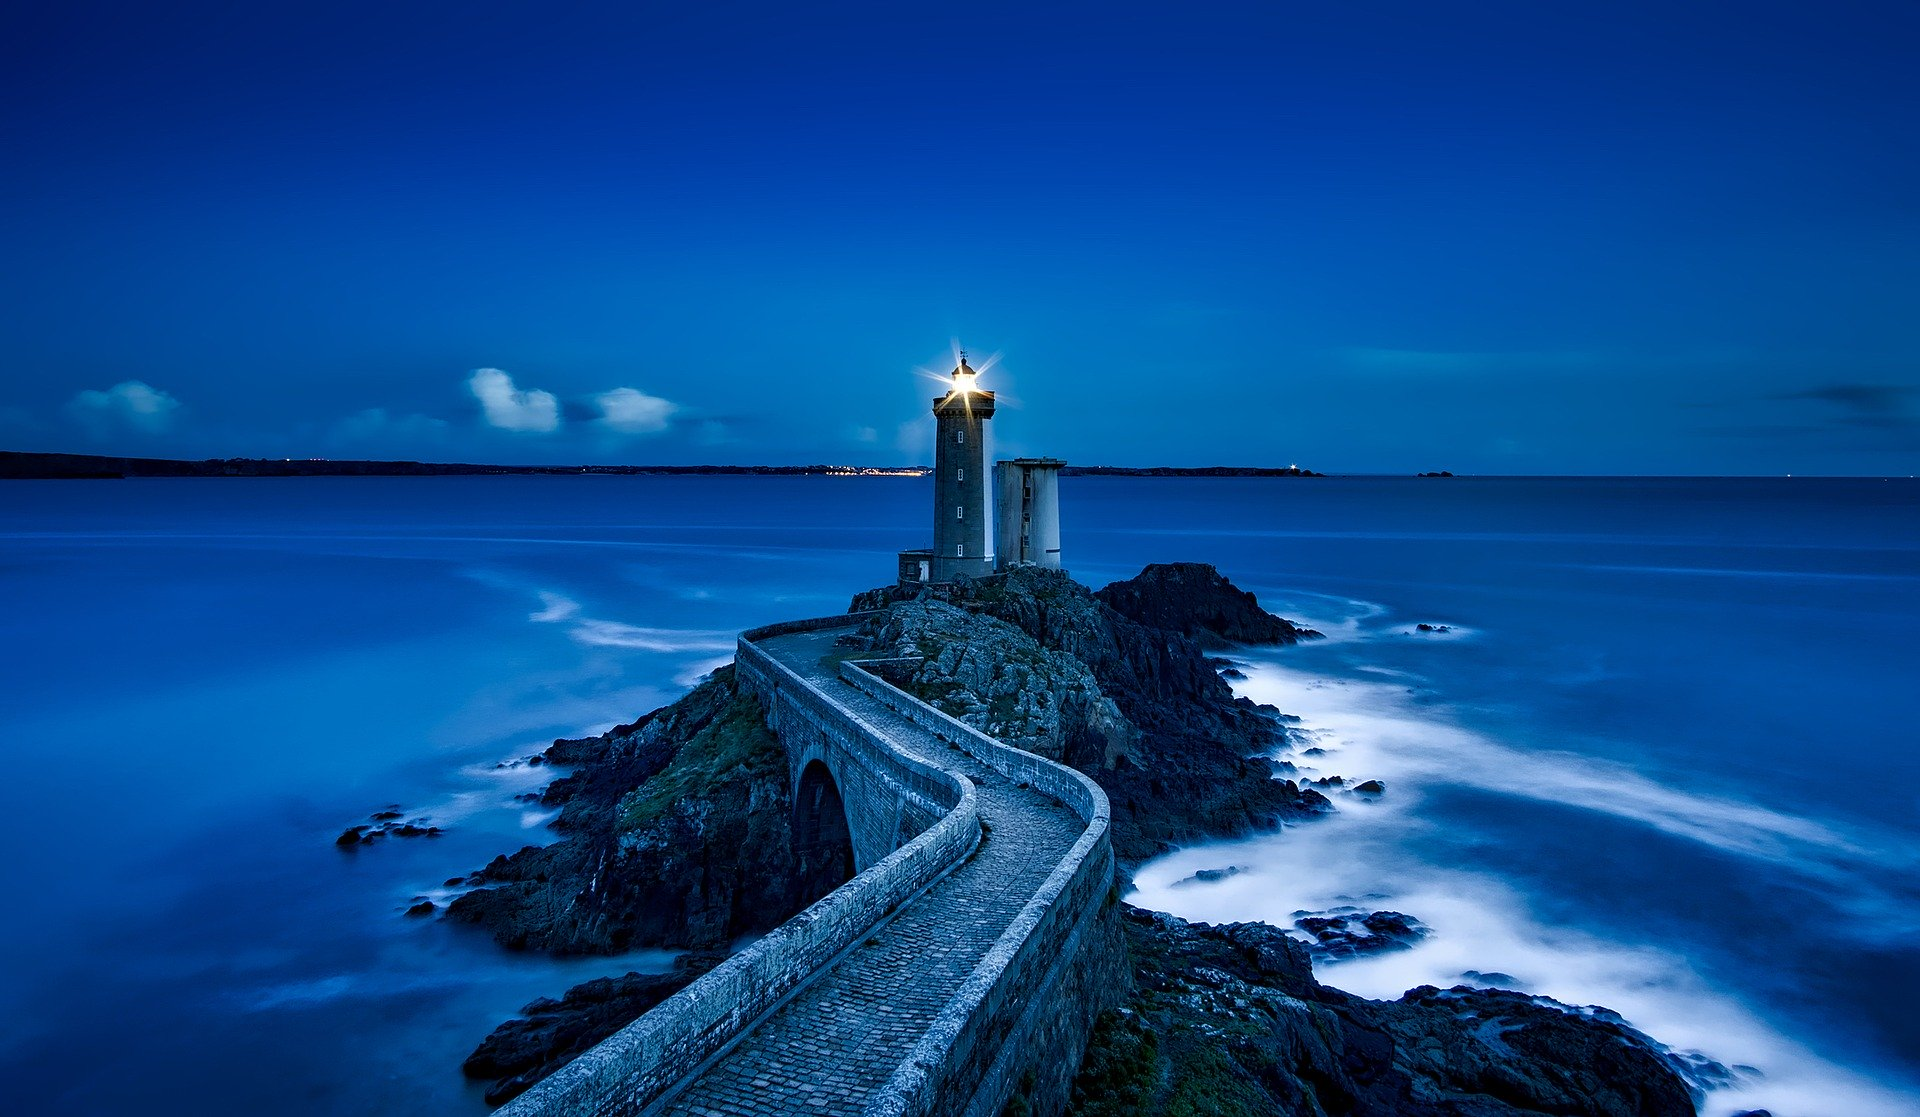
\includegraphics{images/plouzane-1758197_1920.jpg}
    \vspace*{40mm} %%% * is used to give space from top
    \begin{flushright}
        \textbf{\Huge {DevSecOps Tactical}}\\
        \vspace{5mm}
        \Large \textsf{Franklin Diaz}\\
        %\Large \textsf{Created on : April 20, 2020}
        \vspace*{0mm}
        %\Large \textsf{Last updated : \today}
    \end{flushright}
    \clearpage
    \vspace*{\fill}
\end{titlepage}
\justify{}
\textcopyright{} 2021, by Franklin Diaz
\justify{}
Licensed under \href{https://creativecommons.org/licenses/by-nc-nd/4.0/}{CC BY-NC-ND 4.0} 
\faCreativeCommons\ \faCreativeCommonsBy\ \faCreativeCommonsSa\
\vspace{5mm}\\
First Edition 2021
\justify{}
Front cover image design by {\href{https://www.linkedin.com/in/eddiemize/}{Eddie Mize}}.
Images at the beginning of the chapters in this book are
\href{https://pixabay.com/service/terms/#license}{courtesy of Pixabay}
\justify{}
The source for this book is available from 
{\href{https://github.com/thedevilsvoice/devsecops-tactical-book}{devsecops-tactical-book}}
\vspace{3mm}
Published on: \today
\justify{}
This book was initially drafted using the reStructuredText file format.
The Sphinx module for Python was used to format these files and programatically
generate LaTeX, and other working formats used in the typesetting process. The
resultant LaTeX files were managed using TeXstudio.
\justify{}
Some graphs have been generated programatically using the Graphviz software.
The entire publishing environment is developed and maintained according
to the principles outlined in this book.
\vspace{5mm}
\centering
\vspace{0mm}
\begin{figure}[!htb]
	\centering
	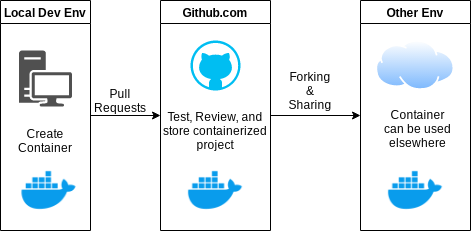
\includegraphics[scale=0.75]{images/workflow.png}
\end{figure}
\vspace{2mm}
Containerized publishing work flow.

%\chapter*{Dedication}
\justify{}
This is where the dedication will be.
\chapter*{Preface}
\addcontentsline{toc}{chapter}{Preface}
\vspace{5mm}

\justify{}
Creation is a long and twisty path, fraught with the distractions of a life well-lived and the frenetic pace of a day and
age that clamors for a million tiny bits of our attention. A supportive and loving family is the touchstone that grounds
us through it all. The author would like to thank his family, especially his loving wife for making it possible to maintain
focus in a focus-stealing world.

\justify{}
Feedback has been a key component in getting these words organized into the order they appear before you today. Thank you to
those folks who contributed their time to review this book including Aaron Didier (@phreakinggeek).

\justify{}
A special thank you to {\href{https://www.linkedin.com/in/eddiemize/}{Eddie Mize} for providing the cover art for this book
and being a good friend.

\justify{}
The ideas captured here are not a means to any particular end. Rather, these are meant to be starting points, giving
you a frame of reference with novel technologies and techniques to streamline your workflows and give your projects
a productivity boost. The hope is the reader will gain momentum to pursue these new ideas by following along with the
examples outlined in this book.

\justify{}
You should work to build up your own solid base of code examples and problem solving techniques that will greatly increase
your efficacy. Over time, new tools and processes will rotate in and out of your toolbox as technology progresses. Keep
in mind that your job is to maintain that momentum, to keep experimenting and to see what is useful enough to stick with
you and make a permanent part of your technical repertoire.

\justify{}
This book is meant to be a workbook as much as it is meant to be read. You are encouraged to jump ahead, go back and re-read,
do the exercises you think you can apply the learning objective from right away, and skip the parts you don't think you will
ever use. Learning can be a non-linear experience and you are encouraged to ``color outside the lines'' to the extent you feel
comfortable doing so. That said, I've attempted to give this book a feel of moving the reader
along towards a final lab project. This project is meant to guide the reader through application of the topics covered before 
the final chapter.

\justify{}
Companies often make their services free in the hopes that you will see the value and usefulness of their products. Their
thinking goes that hopefully you will see enough utility that you will recommend them to your enterprise clients and
integrate their products into your workflows. Not a bad trade-off! It only makes sense to avail yourself of free-tier
cloud services, build and test platforms, and low or no-cost hosting environments. There are plenty of these out there and
we will explore some of these as we dive further into the topics.

\justify{}
When we choose to use a tool, say Ansible\index{Ansible} for example, we must adopt the
most up-to-date and best practices for using that tool. File system layout, naming conventions, script syntax and organization,
and so on. We get to enjoy the clear and safe path forged by the folks that came before us, and with whom we share many goals.
As your skills mature over time, you may want to consider donating time back to the
open source and other communities upon which your knowledge has been built.

\justify{}
Finally, I find it very helpful for my own personal peace of mind to leave projects ``clean and green'', to the extent
possible. In other words, there is mental benefit to tidying up your physical and virtual workspace
before walking away from the keyboard for the day. Perhaps you would find similar benefit should you choose to adopt
this practice.

\tableofcontents
\listoffigures
\listoftables

\mainmatter{}
\chapter{Introduction}

\centering
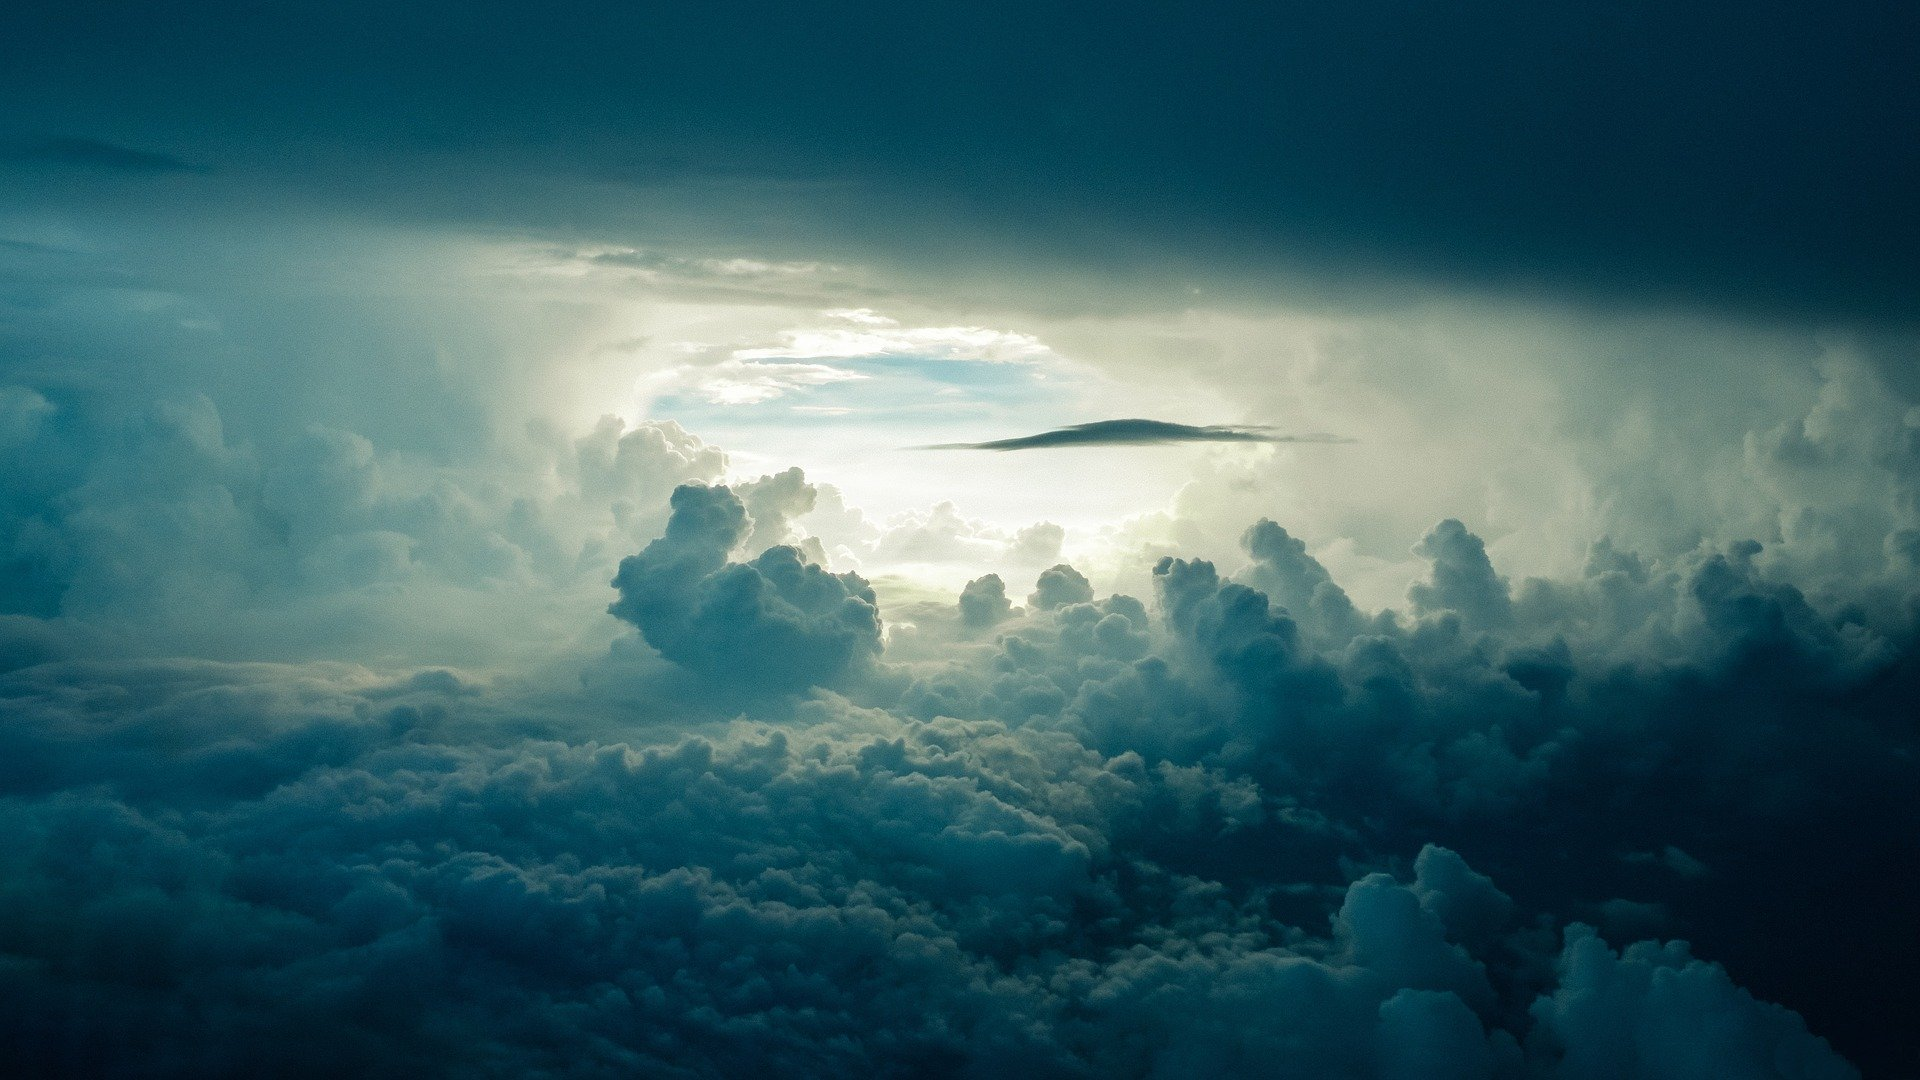
\includegraphics{images/sky-690293_1920.jpg}

\justify{}
The term DevSecOps\index{DevSecOps} is an amalgam of the words Development, Security,
and Operations. The combination of these three words represents the overlap and
interplay between sometimes disparate work functions. The degree to
which these three realms overlap is often a reflection of the structure of a given
organization. Simply put, DevSecOps lives at the intersection of application development
and/or Infrastructure as Code development, Information Security, and Network Operations.

\justify{}
This overlapping DevSecOps job functionality has some overarching goals For
example, the movement software through an ongoing series of incremental test and
deployment phases, which is often referred to as pipelines\index{pipeline}. We will
explore this concept of pipelines and other ways our platforms and infrastructure
are becoming more abstract from the viewpoint of the tools that we use to do it.
Definition of our infrastructure in reusable software patterns is another big objective
in the DevSecOps paradigm. This Infrastructure as Code
(IaC)\index{Infrastructure as Code (IaC)} is the platform
upon which our application software work products flow through a cycle of Continuous
Deployment or Continuous Delivery (CD)\index{Continuous Delivery (CD)}.

\justify{}
Folks at the leading edge in today's computing industry are not just building
software, but are curating it through a cyclical process of continuous development,
testing, use, and improvement. With increasing frequency, applications and
workloads are moving to computing environments that are abstracted away, managed
by invisible armies of engineers who work at companies other than their own. Of course
we are referring to those multitenant cloud type computing landscapes. Passing
one or more fully encapsulated applications to a cloud provider for the purposes
of having ``someone else'' host it as a production environment has become
commonplace. Further, cloud service providers are adding new features and capabilities
at breakneck speed. We are promised our staff will be liberated from burdensome
maintenance tasks for hosts, networks, traffic capacity, storage, and more once
e decide to go ``Cloud Native''. Large amounts of time,
money, and resources are being thrown at cloud migration efforts. Moving away
from traditional networks to those hosted in public
cloud provider environments takes plenty of time, money, planning, and refactoring.
The world is changing with respect to how software is created and maintained.

\begin{figure}[!htb]
	\centering
	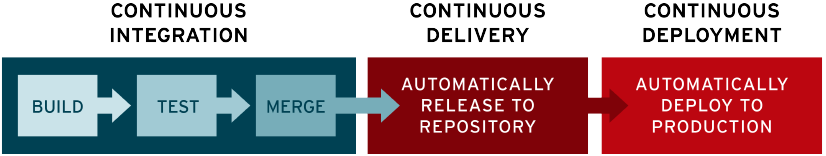
\includegraphics[scale=0.35]{images/ci-cd-flow-desktop_0.png}
	\caption{Typical pipeline stages.}
\label{stages}
\end{figure}

\justify{}
To the extent possible, the modern software project team often aligns around an
attempt to realize gains in performance of our people and projects by
leveraging automation\index{automation} and Agile development practices throughout the
feature development cycle. We aim to reduce complexity, increase consistency, and make
scaling up as smooth as possible, all at once.

\justify{}
At the time of this writing in 2020, about 40\% of production workloads are
running on containers or are deployed in low cost serverless configurations.
Bare metal and virtual machines currently host a bit over 60\% of production
workloads. Containerized workload use is expected to increase even more in
the coming years. Conversely, bare metal and VM usage is expected to
decrease in the coming years. \cite{cnative}

\justify{}
It's not a question of if, but how quickly commoditization of compute resources
will replace private corporate data centers, perhaps resulting in only a
few main providers of cloud computing resources. This shift has been likened
to how power generation and distribution became centralized
in the previous century, now the domain of a few large utility companies.
Nothing beyond considerations of time, money, and practicality stop you
from making your own electricity, but most folks are keen to invest their
efforts in other pursuits.

\justify{}
Strategic decisions are about defining the direction of a team and overseeing
the allocation of the resources needed to pursue the goals of the entire
business organization. These are the sorts of things the upper managers are
thinking about. The linking of the strategic direction to tactical tasks is
done with operational planning. This managerial view might be best framed in
year-long increments. Think of operational planning as the purview of line
and middle managers who detail the goals and milestones, and capture metrics
on progress toward strategic goals of the business. Finally, tactical concerns
are the short range objectives of a team within a department or business unit.
The tactical viewpoint tends to span a time period of one year or less and is
the domain of the individual contributor and technical champion. This is the
``fun stuff'', where you get to be closest to the code. This book will focus
on the practical, by and for those who want to be tactical. There is also
an interdependence on the logistical here. Logistics in our context refers to
the things that make it possible for the tactical to succeed, and look good
while doing it!

\justify{}
Among the tactical practitioners, we can further decompose responsibility into
varying degrees of Development, Security, and Operational work. The typical
person in a developer type role is often working under stringent deadlines to
``ship code'', which means their main focus is ``getting code out the door'' to
keep management happy. Folks in a role that is mainly security focused are mostly
concerned with prevention of the abuse of the technology assets of a business. The
operations type roles have the task of keeping everything up and running, as well as
ensuring all the bits and pieces of technology functioning properly together.

\justify{}
In this book, we will explore a combination of techniques that can enhance and refresh
your skills and align your projects with the technological leading edge. We will
introduce various popular technologies, then use common bits and pieces of
these technologies to get you thinking like a DevSecOps practitioner. We will try out
various code snippets and exercises to build confidence. The ultimate goal is to be able to
create a secure build pipeline for your lab and development work,
test, and even production environments. The techniques here are meant to help
the security-minded developer sharpen her or his skills, and introduce tips
and tactics that benefit the teams they are a part of. There are many, many
ways to reach similar goals these days with the preponderance of Open Source
and commercial tools that are available. By focusing on a few we can blaze a
trail to success in our projects.

\justify{}
Often a distinction is made between folks
who work on the front and back end of software ecosystems. It should be noted that this
book is written by someone with the
experience and perspective of a ``backend'' developer. When we discuss security in this context,
it will typically be a reference to ``infrastructure'' rather than ``application''.

\justify{}
With a goal in mind of selecting complementary tools and process to construct
and streamline our ways of working, we will attempt to leverage these ways in the coming chapters.
There is no clear, definitive moment or milestone we can point to when these ways can be considered
``best practices'', but this is indeed our desired destination.

\begin{displayquote}
\emph{Commercial or professional procedures that are accepted or prescribed as being correct or most effective.}
\href{https://www.oxfordlearnersdictionaries.com/definition/american_english/best-practice}{Oxford English Language Dictionaries}
\end{displayquote}


Along the way we should strive for simplicity and reduction of complexity when possible.
Experience tells us that tools, security measures, and process that are too cumbersome
or otherwise prohibitive in nature are typically circumvented, or even abandoned.
Complexity in our processes become the snags and side projects that are the
enemy of productivity.

\justify{}
Refuse to shave more yaks\cite{yak}
 than absolutely necessary!


\part{Preparation} % part 1
\chapter{Some Big Ideas}

\centering

\includegraphics{12-big-ideas.jpg}

\justifying
There are some key precepts that will serve the aspiring DevSecOps engineer well. In this
chapter we will explore some of these in an attempt to level-set our understanding of the
domain. We will also continue to introduce the reader to the vernacular of the modern day
DevSecOps engineer in a world gone cloudy. You certainly don't need to memorize all of these terms, but the rationale
is they are prevalent enough that you should have a passing familiarity with them, at the very least.

\section{What are DevOps and DevSecOps?}

\justifying
Fundamentally, DevOps and DevSecOps are models for how a team or set of teams can be arranged
to optimize the creation of applications and Infrastructure as Code. They both benefit from
employing similar, if not identical, Agile methodologies. Calling out the ``Security''
piece explicitly in the ``DevSecOps'' nomenclature often signifies an intentional inclusion
of security focused process and activities by the teams involved. Some folks will stick with
the term ``DevOps'', insisting the security piece is still there and just as important, so
there is no need for it to be called out separately.

\justifying
Consider the table \ref{DevSecOps} below. The big takeaway here is to notice the DevSecOps path goes a bit further
in highlighting security and making it a priority. The goal is to think hard about integrating
security and making it a conscious team effort. Adding a security engineer to DevOps design
and review meetings may not be enough to fuse security into our workflows. We want to ensure
our work products are as secure as possible.

\begin{table}[ht]
    \centering
    \begin{tabular}{|l|c|c|}\hline
                                   & DevOps & DevSecOps \\\hline
        Shifting Left              &   X    &    X       \\\hline
        Automated Security Testing &        &    X       \\\hline
        Policy as Code Testing     &        &    X       \\\hline

    \end{tabular}
\caption{DevOps vs. DevSecOps}
\label{DevSecOps}
\end{table}

\section{Revision Control}

\justifying
Code, documents, test cases, and other software work products begin their lives on the workstations of creators
and developers. In this book we will refer to the environments where this takes place as the ``local'' environment.
These work products are typically created, reviewed and checked into Revision Control Systems
(RCS)\index{Revsion Control System (RCS)}, GitHub\index{GitHub} for example, by the DevSecOps practitioner.
Other popular revision control systems include GitLab\index{GitLab} and BitBucket\index{BitBucket}.

\justifying
Although it may seem like there are a lot of choices when it comes to revision control, there is one tool that
underlies them all. That tool is known as git. Git is the brainchild of Linus Torvalds, who also happens to be
the person that invented the Linux kernel just before the turn of the century. This tool work wonderfully on projects small
and large. For this and may other reasons, it is at the heart of many of these RCS systems that we just mentioned. Note that
in addition to these websites, there are many desktop tools meant to aid developers with revision control on their local
machine. While these can be quite handy, there is no substitute for learning the intricacies of git from the command
line. It will come in quite handy indeed.

\justifying
We will look more closely at git and revision control in a later chapter.

\section{Testing}

\justifying
A test case as a discrete check, or grouping of similar types of checks,
that we use to ensure our work products meet certain minimum standards. Test cases are created with
and often run against our work products at the time they are checked in to the revision control system.
This is meant to ensure stability, security, and compatibility with the existing code base in revision
control. The automation required to execute tests every time work is checked in to
revision control is typically the responsibility of the DevSecOps engineers. We will delve into various
types and aspects of testing throughout this book.

\subsection{White Box vs. Black Box Testing}

\justifying
This is a distinction based on whether you have access to the code, documentation, or hardware under test.
For example, testing the code from a project where you can see the source code would be considered "white box"
testing. You might also look at this as the difference between red\index{Red Team} and blue
teaming\index{Blue Team}. For instance, a "red teamer" or "penetration tester" will typically not have
access to documentation about a system that they are testing.

\section{Pipelines}

\begin{figure}[!htb]
\centering
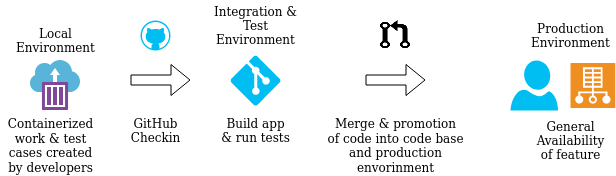
\includegraphics[scale=0.63]{12-flow.png}
\caption{Typical build pipeline}
\label{pipeline}
\end{figure}

\justifying
As seen in figure \ref{pipeline}, work typically flows from the local environments, into a test
environment, and finally to production where it is available for use by the entire user base.

\justifying
We will refer to the entirety of this three-stage flow as one example of what is known as a build pipeline\index{pipeline}.
Code from one or more local environments is checked in to the revision control system throughout a
typical DevSecOps workday, and continuously tested and integrated with the main code base. That is to say, work undergoes
Continuous Integration (CI)\index{Continuous Integration (CI)} with the main code base,
and often Continuous Delivery (CD)\index{Continuous Delivery (CD)} between local, test, and production environments. This is
where the term ``CI/CD Pipeline'' comes from. A business unit may choose to designate more than just the three dev, test,
and prod environments mentioned here, depending on their particular use cases and ways of working.

\justifying
While the CI/CD Pipeline is often a primary focus of the DevSecOps engineer, other pipelines exist as well. For example,
let's assume our organization maintains a vast pool of raw data, also known as a data lake\index{Data Lake}. The staff Data
Engineers build and maintain Data Science\index{Data Science} pipelines to facilitate the smooth flow
of logs and other data into that data lake. Now Data Scientists are able to create machine learning models that rely on that
data to produce useful insights. As another example, consider code changes as they move from
developer workstations into a code repository for storage. Accessing this code for the purpose of testing will differ from
how it is accessed for the purposes of deployment. The order of operations and flow
between differing functions might be said to comprise two different pipelines.

\section{Automation}

\justifying
Consider what may happen when we want to apply the lessons from this book across a large environment made up of many hosts,
containers, pieces of application software, etc. It becomes a huge challenge for an operator to log in to each host or container
individually. Typing, or even cutting and pasting commands to keep things up and running properly, look at logs,
and so on becomes problematic. Creating shell scripts can be quite helpful, but is an outdated modality when we consider
the daunting size and complexity of the modern administrative domain.

\justifying
This is a great use-case for automation. Automation\index{automation} is a way to provision and maintain some or many hosts
in a programmatic manner. Another desirable goal, and hopefully result of automation is to reduce the amount of
per-host interaction that comes with the work of administering systems. Automation is the force multiplier we use to achieve
scaling\index{scaling}. As DevSecOps practitioners, we are on a never-ending quest to achieve
scale-invariance\index{scale-invariance}, to borrow a term from the mathematical realm. That is to say, the tools we
build and processes we engender should work just as well for three machines as they do for three thousand.

\section{Scalability}

\justifying
Bringing together many of the ideas in this section as a foundation, we're able to serve our pipelines and applications from a few users, to many.
Consider the differences between the sort of traffic we can handle with an application on a single server, compared to the
amount of traffic we can handle when we introduce five more servers running the same application code, and a load balancer
to distribute the traffic evenly among these servers.

\justifying
Couple the principle of scalability with the explosive automation tooling ecosystem and you are on the path to doing more,
better work in less time with a smaller staff.

\section{Immutability}

\justifying
There is obvious advantage of being able to quickly stand up new clones of our project to replace existing instances that
may be outdated, insecure, etc. The idea of immutability, in reference to software projects, is the degree to which something,
our running project for example, can be changed. Immutability\index{immutability} is desirable, in that we wish to be able to
simply replace outdated instances of our project in their entirety. Upgrading and patching are inherently
problematic activities, high cost in terms of time, effort and money, that we have the technology to dissociate from. With
containerization, we can more easily achieve immutability across the software life cycle.

\section{Ephemerality}

\justifying
Ephemerality\index{ephemerality} is the concept of something being inherently transitory in nature. For something to be
considered ephemeral, it can exist only briefly. Using immutable containers makes it easier to realize
infrastructure and hosts that are ephemeral. Rather than spending a great deal of time patching and upgrading systems as
we might in a traditional project stack that uses bare metal hosts or even virtual machines, we're going to
use Docker to create a new container in place of the old one. In other words, we're running our project in containers that
are immutable and ephemeral to the degree possible.

\section{GitOps}

\justifying
Just to be sure we have a complete picture of the landscape, we will define the term ``GitOps''\index{GitOps} as a
cloud native analog of Infrastructure as Code being developed with the DevOps/DevSecOps paradigm. Cloud infrastructure
stored in a Git based revision control system can keep a Kubernetes cluster up to date, often with Continuous Deployment.

\section{Organizational Maturity}

\justifying
When I first encounter a new team or group, I try to frame their capabilities in terms of organizational maturity.
Many things can have an effect on the posture of an organization. A few examples:

\begin{itemize}
	\item How many team members there are.
	\item How and how often they interact.
	\item  What productivity tools do they use?
	\item How often and Why do they meet?
	\item How their work is captured, completed, and reviewed?
\end{itemize}

The structure of a team and the tendency to follow best practices, as well as their own policies, tend to provide some
valuable insight. The measure of these insights is the maturity of the team. Even a cursory and informal aanalysis can give
a sense of challenges that might arise during creation of work products in terms of time, potential quality, and of course,
the security of any output. The importance of the maturiy of an organization stems from it's high degree to which it shapes
the effectiveness of that organization.

\justifying
Let's consider Conway's Law:

\begin{displayquote}
    \emph{Any organization that designs a system (defined broadly) will produce a design whose structure is a copy of the
organization's communication structure.}

Melvin E. Conway
\end{displayquote}

\justifying
As with so many things in life, communication is a fundamental key to team success. Keep in mind that each DevSecOps
team is somewhere on the spectrum in terms of their capability and organizational maturity, whether they realize it or not!
There is a direct correlation between the maturity of the team and the results you will get from them. Of course there are
plenty of decent blogs and articles on the web that provide detail on the ``DevSecOps Maturity Model'' in case you want to
dig deeper on this subject.

\chapter{Getting Ready to Get Tactical}

\centering

\includegraphics[scale=0.20]{images/ingredients-498199_1920.jpg}


\justify{}
Think of this chapter as the \emph{mise en place} of our DevSecOps souffle. We will increase our chances of success
by preparing our work environment for the project at hand. Let's start our preparations by outlining our
overall objectives. We want to:

\justify{}
\begin{itemize}
	\item
	      Create an extensible lab environment for rapid prototyping and development.
	\item
	      Keep our lab costs down while meeting the rest of the objectives.
	      Utilize free services and open source tools to the extent possible.
	\item
	      Use the published best practices for each tooling, operations, or
	      development ecosystem we choose to employ.
	\item
	      Always leave our projects in a functional state.
	\item
	      Get out of our old comfort zone, into a new one.
\end{itemize}

\section{Prerequisites}

\justify{}
This book intends to be a practical treatment of common and popular technologies from the DevSecOps world. As such, we assume
the reader has some basic knowledge of certain concepts. We will be exploring new ways of working for folks who
are somewhat familiar with:

\begin{itemize}
	\item
	    Linux (UI and command line)
	\item 
        Python 3
	\item
	    Familiarity with github.com and the concepts of pull requests and branching.
\end{itemize}

\justify{}
The examples in this book have been tested on Linux running the latest version of Docker. For more
intformation about installing Docker, see \href{https://docs.docker.com/get-docker/}{the Get Docker section}
of their website. There are directions there for installing Docker on Linux, Mac, and other operating systems.

Let's take a look at some of the other foundational environmental elements we need in place to be successful.

\section{Packages}

\subsection{MacOS}

Homebrew bills itself as \href{https://brew.sh/}{the missing package manager for MacOS}. Using ``brew'' and also
``cask'' to install and manage packages on MacOS will make your life much simpler.

\justify{}
It is also recommended that you familiarize yourself with the Terminal application on MacOS. Note that brew
commands are executed form within the terminal rather than using the GUI. Also bear in mind that packages are
installed with your user account. In other words, ``SuperUser'' privileges are not just discouraged, they are
neither required nor desired.

\subsection{Linux}

My prefered environment is a Debian based Linux distribution. Ubuntu, Cinnamon, and PopOS are all examples of 
Linux distrubutions in this family. While some code examples and lab containers use Debian-based distros, you
may also encounter Alpine Linux (typically chosen for it's smaller image size), amoung others.

\section{The Workhorse (IDE)}

\begin{figure}[!htb]
\centering
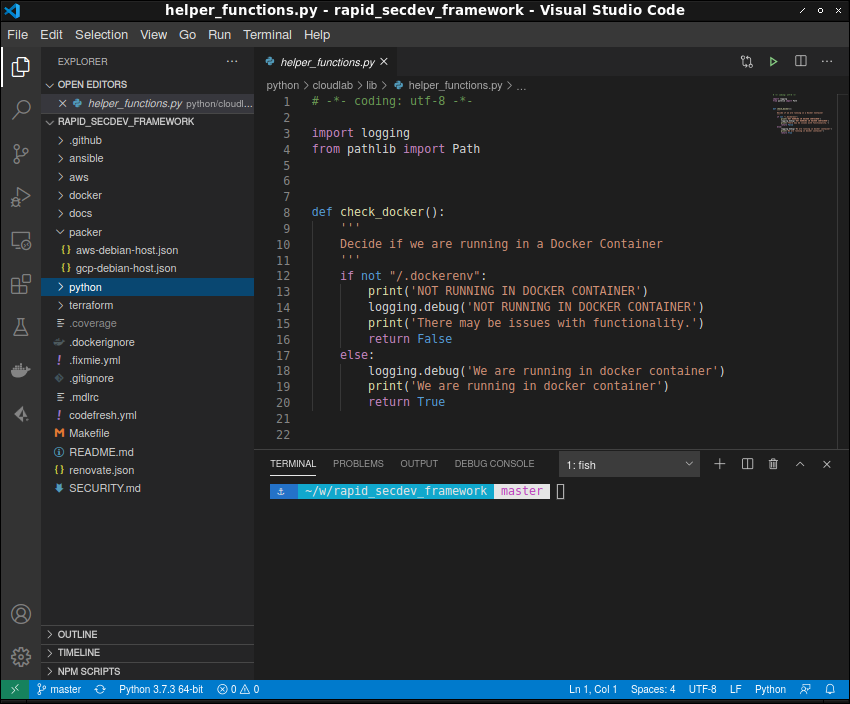
\includegraphics[scale=0.45]{images/setup-vscode.png}
\caption{The VScode IDE.}
\label{vscode-ide}
\end{figure}

\justify{}
It is quite helpful to have a piece of software on your workstation that makes code and document creation and edits easier. This
software is commonly known as an Integrated Development Environment (IDE)\index{IDE}. A decent IDE with the right add-ons can
provide syntax highlighting to show potential issues you might have missed, help you check for spelling or
grammar mistakes in your documentation, and even makes suggestions on alternate ways of writing your code.

\justify{}
There are many commercial and Open Source IDEs available. Visual Studio Code from Microsoft is a popular choice due to it's easy
installation. VSCode\index{VSCode} works well on Linux, Mac and other operating systems.
The environment is easily extensible to support most any language, linter, or syntax checker we may have a need
for, thanks to their easy to use and well integrated ``Extension'' feature. VSCode also has an integrated terminal
window\index{Terminal Window} so the developer can execute shell commands without leaving the IDE screen.

\section{SSH Key Setup}

\justify{}
Take note of the fact that setting up SSH keys means generating a pair of keys, not a single key. This is an important 
distinction. You will want to add your public key to sites like \href{github.com}{github.com}. The public key half will
also be added to machine instances that you create with public cloud providers. This will allow you to log in without
having to provision a user/password combination. You should take care to 
protect the private key at all times. Under no circumstances should you share your private SSH key.\cite{ssh}
\justify{}
Take a few minutes to generate an SSH key\index{SSH keys} pair if you don't already have one. We will add the public half of
our SSH key pair to hosts we provision. The directions for generating an SSH keypair found on the
\href{github.com}{github.com} website are perfect for our setup task. Follow the directions in the article 
\href{https://docs.github.com/en/github/authenticating-to-github/connecting-to-github-with-ssh/generating-a-new-ssh-key-and-adding-it-to-the-ssh-agent}{Generating a new SSH key and adding it to the ssh-agent}

\subsection{Generating a Key from the Command Line}

If you are using a Linux or Mac system, you have the option to create your SSH key pair from the command line. Consider 
the following example code listing.

\begin{mybox}{\thetcbcounter: SSH Key Generation}
\lstinputlisting{code/13-setup/ssh-key-generation}
\end{mybox}

\justify{}
Now you can add your public key half to your user settings in \href{github.com}{github.com}. For me it makes sense to have
two key pairs, one used for work projects, and one used for personal projects.

\section{GPG Key Setup}

\justify{}
\href{https://gnupg.org/}{Gnu Privacy Guard (GPG)} is an Open Source replacement for Symantec's PGP software. It allows you
to generate an asymmetric key pair that can be exchanged with other users, encrypt your personal files, or verify your identity.
Again, you will want to be sure to share your public key and protect your private key. This is the same reasoning we used in the
case of our SSH keys.

\justify{}
We will use a GPG key to sign commits to GitHub\index{GitHub}. This will help others verify that work you check in to revision
control did actually come from you. It's not strictly necessary but is considered good practice.
Some repositories require that you sign your pull requests with your GPG key\index{GPG key}.

\justify{}
Take a few minutes to set up a GPG key. Once you have an account setup, you can add
it to your profile on \href{github.com}{github.com}.

\subsection{Command Line GPG Key Setup}

\begin{mybox}{\thetcbcounter: Command Line GPG Key Setup}
\lstinputlisting{code/13-setup/gpg-key-setup}
\end{mybox}

\justify{}
Copy your GPG key, beginning with the string ``BEGIN PGP PUBLIC KEY BLOCK'' and ending with the string
``END PGP PUBLIC KEY BLOCK''. Add the GPG key to your GitHub account.

\section{Using pass to Encrypt Secrets Locally}

\justify{}
The pass program allows you to encrypt your keys, files, and other secrets in an encrypted database that is
stored in your home directory. Know that eventually, secrets leak. They can be exposed in a variety of ways, 
often they are committed to revision control by mistake.

\justify{}
Consider the following example where the pass program is used to encrypt secrets from a terminal window.

\begin{mybox}{\thetcbcounter: Encrypt Local Secrets on your Mac}
\lstinputlisting{code/13-setup/pass-mgr}
\end{mybox}

\section{Standard Project Layout}

\justify{}
The code examples in this book are organized in a standard way. The use of a known project 
layout across all project/repository directories increases the degree to which our projects can be used, reused, and
interoperate. Attention will be called to the folder and file naming conventions that are defined by this layout
as we encounter them.

\section{Installing Docker}

\justify{}
Recall that a properly functioning Docker setup on your local machine is a requirement for the upcoming
lab exercises. See the Docker website for 
\href{https://docs.docker.com/get-docker/}{instructions on how to install and configure Docker}. 

% include markdown file to populate a chapter with a lab from markdown files
\markdownInput{../labs/ch3/lab-3a.md}

\markdownInput{../labs/ch3/lab-3b.md}

\section{Directory Structure}

\justify{}
Relevant files and folders mentioned in this chapter are organized as seen below.

\begin{figure}[!htb]
	\centering
	\chapter{Getting Ready to Get Tactical}

\centering

\includegraphics[scale=0.20]{images/ingredients-498199_1920.jpg}


\justify{}
Think of this chapter as the \emph{mise en place} of our DevSecOps souffle. We will increase our chances of success
by preparing our work environment for the project at hand. Let's start our preparations by outlining our
overall objectives. We want to:

\justify{}
\begin{itemize}
	\item
	      Create an extensible lab environment for rapid prototyping and development.
	\item
	      Keep our lab costs down while meeting the rest of the objectives.
	      Utilize free services and open source tools to the extent possible.
	\item
	      Use the published best practices for each tooling, operations, or
	      development ecosystem we choose to employ.
	\item
	      Always leave our projects in a functional state.
	\item
	      Get out of our old comfort zone, into a new one.
\end{itemize}

\section{Prerequisites}

\justify{}
This book intends to be a practical treatment of common and popular technologies from the DevSecOps world. As such, we assume
the reader has some basic knowledge of certain concepts. We will be exploring new ways of working for folks who
are somewhat familiar with:

\begin{itemize}
	\item
	    Linux (UI and command line)
	\item 
        Python 3
	\item
	    Familiarity with github.com and the concepts of pull requests and branching.
\end{itemize}

\justify{}
The examples in this book have been tested on Linux running the latest version of Docker. For more
intformation about installing Docker, see \href{https://docs.docker.com/get-docker/}{the Get Docker section}
of their website. There are directions there for installing Docker on Linux, Mac, and other operating systems.

Let's take a look at some of the other foundational environmental elements we need in place to be successful.

\section{Packages}

\subsection{MacOS}

Homebrew bills itself as \href{https://brew.sh/}{the missing package manager for MacOS}. Using ``brew'' and also
``cask'' to install and manage packages on MacOS will make your life much simpler.

\justify{}
It is also recommended that you familiarize yourself with the Terminal application on MacOS. Note that brew
commands are executed form within the terminal rather than using the GUI. Also bear in mind that packages are
installed with your user account. In other words, ``SuperUser'' privileges are not just discouraged, they are
neither required nor desired.

\subsection{Linux}

My prefered environment is a Debian based Linux distribution. Ubuntu, Cinnamon, and PopOS are all examples of 
Linux distrubutions in this family. While some code examples and lab containers use Debian-based distros, you
may also encounter Alpine Linux (typically chosen for it's smaller image size), amoung others.

\section{The Workhorse (IDE)}

\begin{figure}[!htb]
\centering
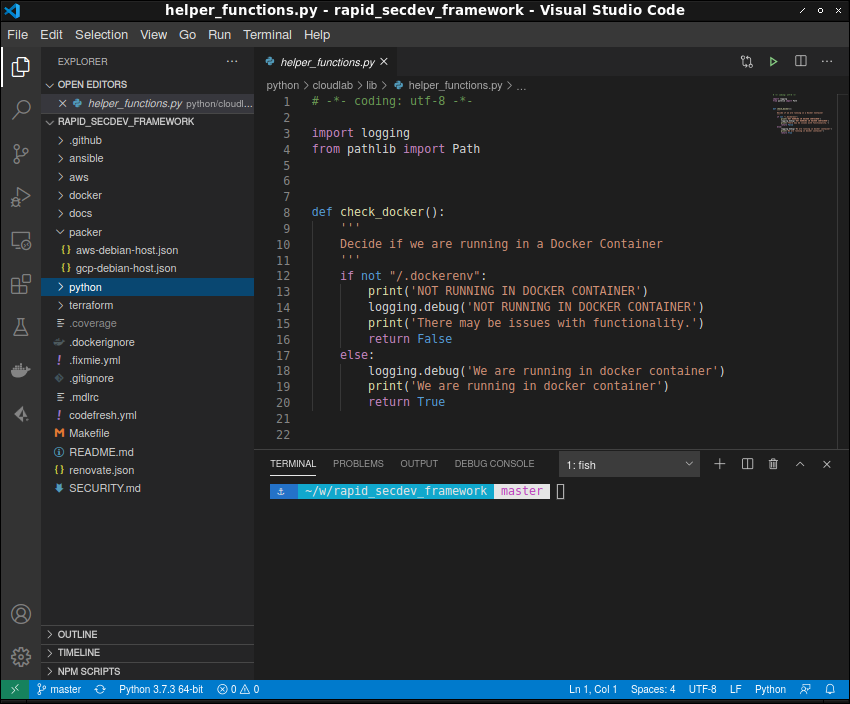
\includegraphics[scale=0.45]{images/setup-vscode.png}
\caption{The VScode IDE.}
\label{vscode-ide}
\end{figure}

\justify{}
It is quite helpful to have a piece of software on your workstation that makes code and document creation and edits easier. This
software is commonly known as an Integrated Development Environment (IDE)\index{IDE}. A decent IDE with the right add-ons can
provide syntax highlighting to show potential issues you might have missed, help you check for spelling or
grammar mistakes in your documentation, and even makes suggestions on alternate ways of writing your code.

\justify{}
There are many commercial and Open Source IDEs available. Visual Studio Code from Microsoft is a popular choice due to it's easy
installation. VSCode\index{VSCode} works well on Linux, Mac and other operating systems.
The environment is easily extensible to support most any language, linter, or syntax checker we may have a need
for, thanks to their easy to use and well integrated ``Extension'' feature. VSCode also has an integrated terminal
window\index{Terminal Window} so the developer can execute shell commands without leaving the IDE screen.

\section{SSH Key Setup}

\justify{}
Take note of the fact that setting up SSH keys means generating a pair of keys, not a single key. This is an important 
distinction. You will want to add your public key to sites like \href{github.com}{github.com}. The public key half will
also be added to machine instances that you create with public cloud providers. This will allow you to log in without
having to provision a user/password combination. You should take care to 
protect the private key at all times. Under no circumstances should you share your private SSH key.\cite{ssh}
\justify{}
Take a few minutes to generate an SSH key\index{SSH keys} pair if you don't already have one. We will add the public half of
our SSH key pair to hosts we provision. The directions for generating an SSH keypair found on the
\href{github.com}{github.com} website are perfect for our setup task. Follow the directions in the article 
\href{https://docs.github.com/en/github/authenticating-to-github/connecting-to-github-with-ssh/generating-a-new-ssh-key-and-adding-it-to-the-ssh-agent}{Generating a new SSH key and adding it to the ssh-agent}

\subsection{Generating a Key from the Command Line}

If you are using a Linux or Mac system, you have the option to create your SSH key pair from the command line. Consider 
the following example code listing.

\begin{mybox}{\thetcbcounter: SSH Key Generation}
\lstinputlisting{code/13-setup/ssh-key-generation}
\end{mybox}

\justify{}
Now you can add your public key half to your user settings in \href{github.com}{github.com}. For me it makes sense to have
two key pairs, one used for work projects, and one used for personal projects.

\section{GPG Key Setup}

\justify{}
\href{https://gnupg.org/}{Gnu Privacy Guard (GPG)} is an Open Source replacement for Symantec's PGP software. It allows you
to generate an asymmetric key pair that can be exchanged with other users, encrypt your personal files, or verify your identity.
Again, you will want to be sure to share your public key and protect your private key. This is the same reasoning we used in the
case of our SSH keys.

\justify{}
We will use a GPG key to sign commits to GitHub\index{GitHub}. This will help others verify that work you check in to revision
control did actually come from you. It's not strictly necessary but is considered good practice.
Some repositories require that you sign your pull requests with your GPG key\index{GPG key}.

\justify{}
Take a few minutes to set up a GPG key. Once you have an account setup, you can add
it to your profile on \href{github.com}{github.com}.

\subsection{Command Line GPG Key Setup}

\begin{mybox}{\thetcbcounter: Command Line GPG Key Setup}
\lstinputlisting{code/13-setup/gpg-key-setup}
\end{mybox}

\justify{}
Copy your GPG key, beginning with the string ``BEGIN PGP PUBLIC KEY BLOCK'' and ending with the string
``END PGP PUBLIC KEY BLOCK''. Add the GPG key to your GitHub account.

\section{Using pass to Encrypt Secrets Locally}

\justify{}
The pass program allows you to encrypt your keys, files, and other secrets in an encrypted database that is
stored in your home directory. Know that eventually, secrets leak. They can be exposed in a variety of ways, 
often they are committed to revision control by mistake.

\justify{}
Consider the following example where the pass program is used to encrypt secrets from a terminal window.

\begin{mybox}{\thetcbcounter: Encrypt Local Secrets on your Mac}
\lstinputlisting{code/13-setup/pass-mgr}
\end{mybox}

\section{Standard Project Layout}

\justify{}
The code examples in this book are organized in a standard way. The use of a known project 
layout across all project/repository directories increases the degree to which our projects can be used, reused, and
interoperate. Attention will be called to the folder and file naming conventions that are defined by this layout
as we encounter them.

\section{Installing Docker}

\justify{}
Recall that a properly functioning Docker setup on your local machine is a requirement for the upcoming
lab exercises. See the Docker website for 
\href{https://docs.docker.com/get-docker/}{instructions on how to install and configure Docker}. 

% include markdown file to populate a chapter with a lab from markdown files
\markdownInput{../labs/ch3/lab-3a.md}

\markdownInput{../labs/ch3/lab-3b.md}

\section{Directory Structure}

\justify{}
Relevant files and folders mentioned in this chapter are organized as seen below.

\begin{figure}[!htb]
	\centering
	\chapter{Getting Ready to Get Tactical}

\centering

\includegraphics[scale=0.20]{images/ingredients-498199_1920.jpg}


\justify{}
Think of this chapter as the \emph{mise en place} of our DevSecOps souffle. We will increase our chances of success
by preparing our work environment for the project at hand. Let's start our preparations by outlining our
overall objectives. We want to:

\justify{}
\begin{itemize}
	\item
	      Create an extensible lab environment for rapid prototyping and development.
	\item
	      Keep our lab costs down while meeting the rest of the objectives.
	      Utilize free services and open source tools to the extent possible.
	\item
	      Use the published best practices for each tooling, operations, or
	      development ecosystem we choose to employ.
	\item
	      Always leave our projects in a functional state.
	\item
	      Get out of our old comfort zone, into a new one.
\end{itemize}

\section{Prerequisites}

\justify{}
This book intends to be a practical treatment of common and popular technologies from the DevSecOps world. As such, we assume
the reader has some basic knowledge of certain concepts. We will be exploring new ways of working for folks who
are somewhat familiar with:

\begin{itemize}
	\item
	    Linux (UI and command line)
	\item 
        Python 3
	\item
	    Familiarity with github.com and the concepts of pull requests and branching.
\end{itemize}

\justify{}
The examples in this book have been tested on Linux running the latest version of Docker. For more
intformation about installing Docker, see \href{https://docs.docker.com/get-docker/}{the Get Docker section}
of their website. There are directions there for installing Docker on Linux, Mac, and other operating systems.

Let's take a look at some of the other foundational environmental elements we need in place to be successful.

\section{Packages}

\subsection{MacOS}

Homebrew bills itself as \href{https://brew.sh/}{the missing package manager for MacOS}. Using ``brew'' and also
``cask'' to install and manage packages on MacOS will make your life much simpler.

\justify{}
It is also recommended that you familiarize yourself with the Terminal application on MacOS. Note that brew
commands are executed form within the terminal rather than using the GUI. Also bear in mind that packages are
installed with your user account. In other words, ``SuperUser'' privileges are not just discouraged, they are
neither required nor desired.

\subsection{Linux}

My prefered environment is a Debian based Linux distribution. Ubuntu, Cinnamon, and PopOS are all examples of 
Linux distrubutions in this family. While some code examples and lab containers use Debian-based distros, you
may also encounter Alpine Linux (typically chosen for it's smaller image size), amoung others.

\section{The Workhorse (IDE)}

\begin{figure}[!htb]
\centering
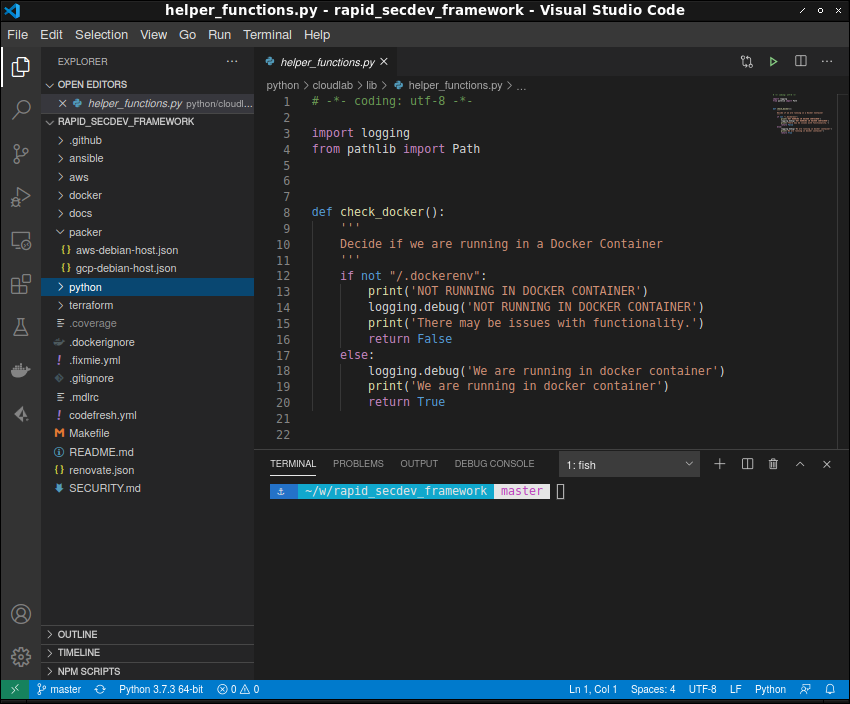
\includegraphics[scale=0.45]{images/setup-vscode.png}
\caption{The VScode IDE.}
\label{vscode-ide}
\end{figure}

\justify{}
It is quite helpful to have a piece of software on your workstation that makes code and document creation and edits easier. This
software is commonly known as an Integrated Development Environment (IDE)\index{IDE}. A decent IDE with the right add-ons can
provide syntax highlighting to show potential issues you might have missed, help you check for spelling or
grammar mistakes in your documentation, and even makes suggestions on alternate ways of writing your code.

\justify{}
There are many commercial and Open Source IDEs available. Visual Studio Code from Microsoft is a popular choice due to it's easy
installation. VSCode\index{VSCode} works well on Linux, Mac and other operating systems.
The environment is easily extensible to support most any language, linter, or syntax checker we may have a need
for, thanks to their easy to use and well integrated ``Extension'' feature. VSCode also has an integrated terminal
window\index{Terminal Window} so the developer can execute shell commands without leaving the IDE screen.

\section{SSH Key Setup}

\justify{}
Take note of the fact that setting up SSH keys means generating a pair of keys, not a single key. This is an important 
distinction. You will want to add your public key to sites like \href{github.com}{github.com}. The public key half will
also be added to machine instances that you create with public cloud providers. This will allow you to log in without
having to provision a user/password combination. You should take care to 
protect the private key at all times. Under no circumstances should you share your private SSH key.\cite{ssh}
\justify{}
Take a few minutes to generate an SSH key\index{SSH keys} pair if you don't already have one. We will add the public half of
our SSH key pair to hosts we provision. The directions for generating an SSH keypair found on the
\href{github.com}{github.com} website are perfect for our setup task. Follow the directions in the article 
\href{https://docs.github.com/en/github/authenticating-to-github/connecting-to-github-with-ssh/generating-a-new-ssh-key-and-adding-it-to-the-ssh-agent}{Generating a new SSH key and adding it to the ssh-agent}

\subsection{Generating a Key from the Command Line}

If you are using a Linux or Mac system, you have the option to create your SSH key pair from the command line. Consider 
the following example code listing.

\begin{mybox}{\thetcbcounter: SSH Key Generation}
\lstinputlisting{code/13-setup/ssh-key-generation}
\end{mybox}

\justify{}
Now you can add your public key half to your user settings in \href{github.com}{github.com}. For me it makes sense to have
two key pairs, one used for work projects, and one used for personal projects.

\section{GPG Key Setup}

\justify{}
\href{https://gnupg.org/}{Gnu Privacy Guard (GPG)} is an Open Source replacement for Symantec's PGP software. It allows you
to generate an asymmetric key pair that can be exchanged with other users, encrypt your personal files, or verify your identity.
Again, you will want to be sure to share your public key and protect your private key. This is the same reasoning we used in the
case of our SSH keys.

\justify{}
We will use a GPG key to sign commits to GitHub\index{GitHub}. This will help others verify that work you check in to revision
control did actually come from you. It's not strictly necessary but is considered good practice.
Some repositories require that you sign your pull requests with your GPG key\index{GPG key}.

\justify{}
Take a few minutes to set up a GPG key. Once you have an account setup, you can add
it to your profile on \href{github.com}{github.com}.

\subsection{Command Line GPG Key Setup}

\begin{mybox}{\thetcbcounter: Command Line GPG Key Setup}
\lstinputlisting{code/13-setup/gpg-key-setup}
\end{mybox}

\justify{}
Copy your GPG key, beginning with the string ``BEGIN PGP PUBLIC KEY BLOCK'' and ending with the string
``END PGP PUBLIC KEY BLOCK''. Add the GPG key to your GitHub account.

\section{Using pass to Encrypt Secrets Locally}

\justify{}
The pass program allows you to encrypt your keys, files, and other secrets in an encrypted database that is
stored in your home directory. Know that eventually, secrets leak. They can be exposed in a variety of ways, 
often they are committed to revision control by mistake.

\justify{}
Consider the following example where the pass program is used to encrypt secrets from a terminal window.

\begin{mybox}{\thetcbcounter: Encrypt Local Secrets on your Mac}
\lstinputlisting{code/13-setup/pass-mgr}
\end{mybox}

\section{Standard Project Layout}

\justify{}
The code examples in this book are organized in a standard way. The use of a known project 
layout across all project/repository directories increases the degree to which our projects can be used, reused, and
interoperate. Attention will be called to the folder and file naming conventions that are defined by this layout
as we encounter them.

\section{Installing Docker}

\justify{}
Recall that a properly functioning Docker setup on your local machine is a requirement for the upcoming
lab exercises. See the Docker website for 
\href{https://docs.docker.com/get-docker/}{instructions on how to install and configure Docker}. 

% include markdown file to populate a chapter with a lab from markdown files
\markdownInput{../labs/ch3/lab-3a.md}

\markdownInput{../labs/ch3/lab-3b.md}

\section{Directory Structure}

\justify{}
Relevant files and folders mentioned in this chapter are organized as seen below.

\begin{figure}[!htb]
	\centering
	\input{dot/13-setup.tex}
	\caption{Setup related files.}
	\label{setupfiles}
\end{figure}


	\caption{Setup related files.}
	\label{setupfiles}
\end{figure}


	\caption{Setup related files.}
	\label{setupfiles}
\end{figure}



\part{Development} % part 2
\chapter{Containers}

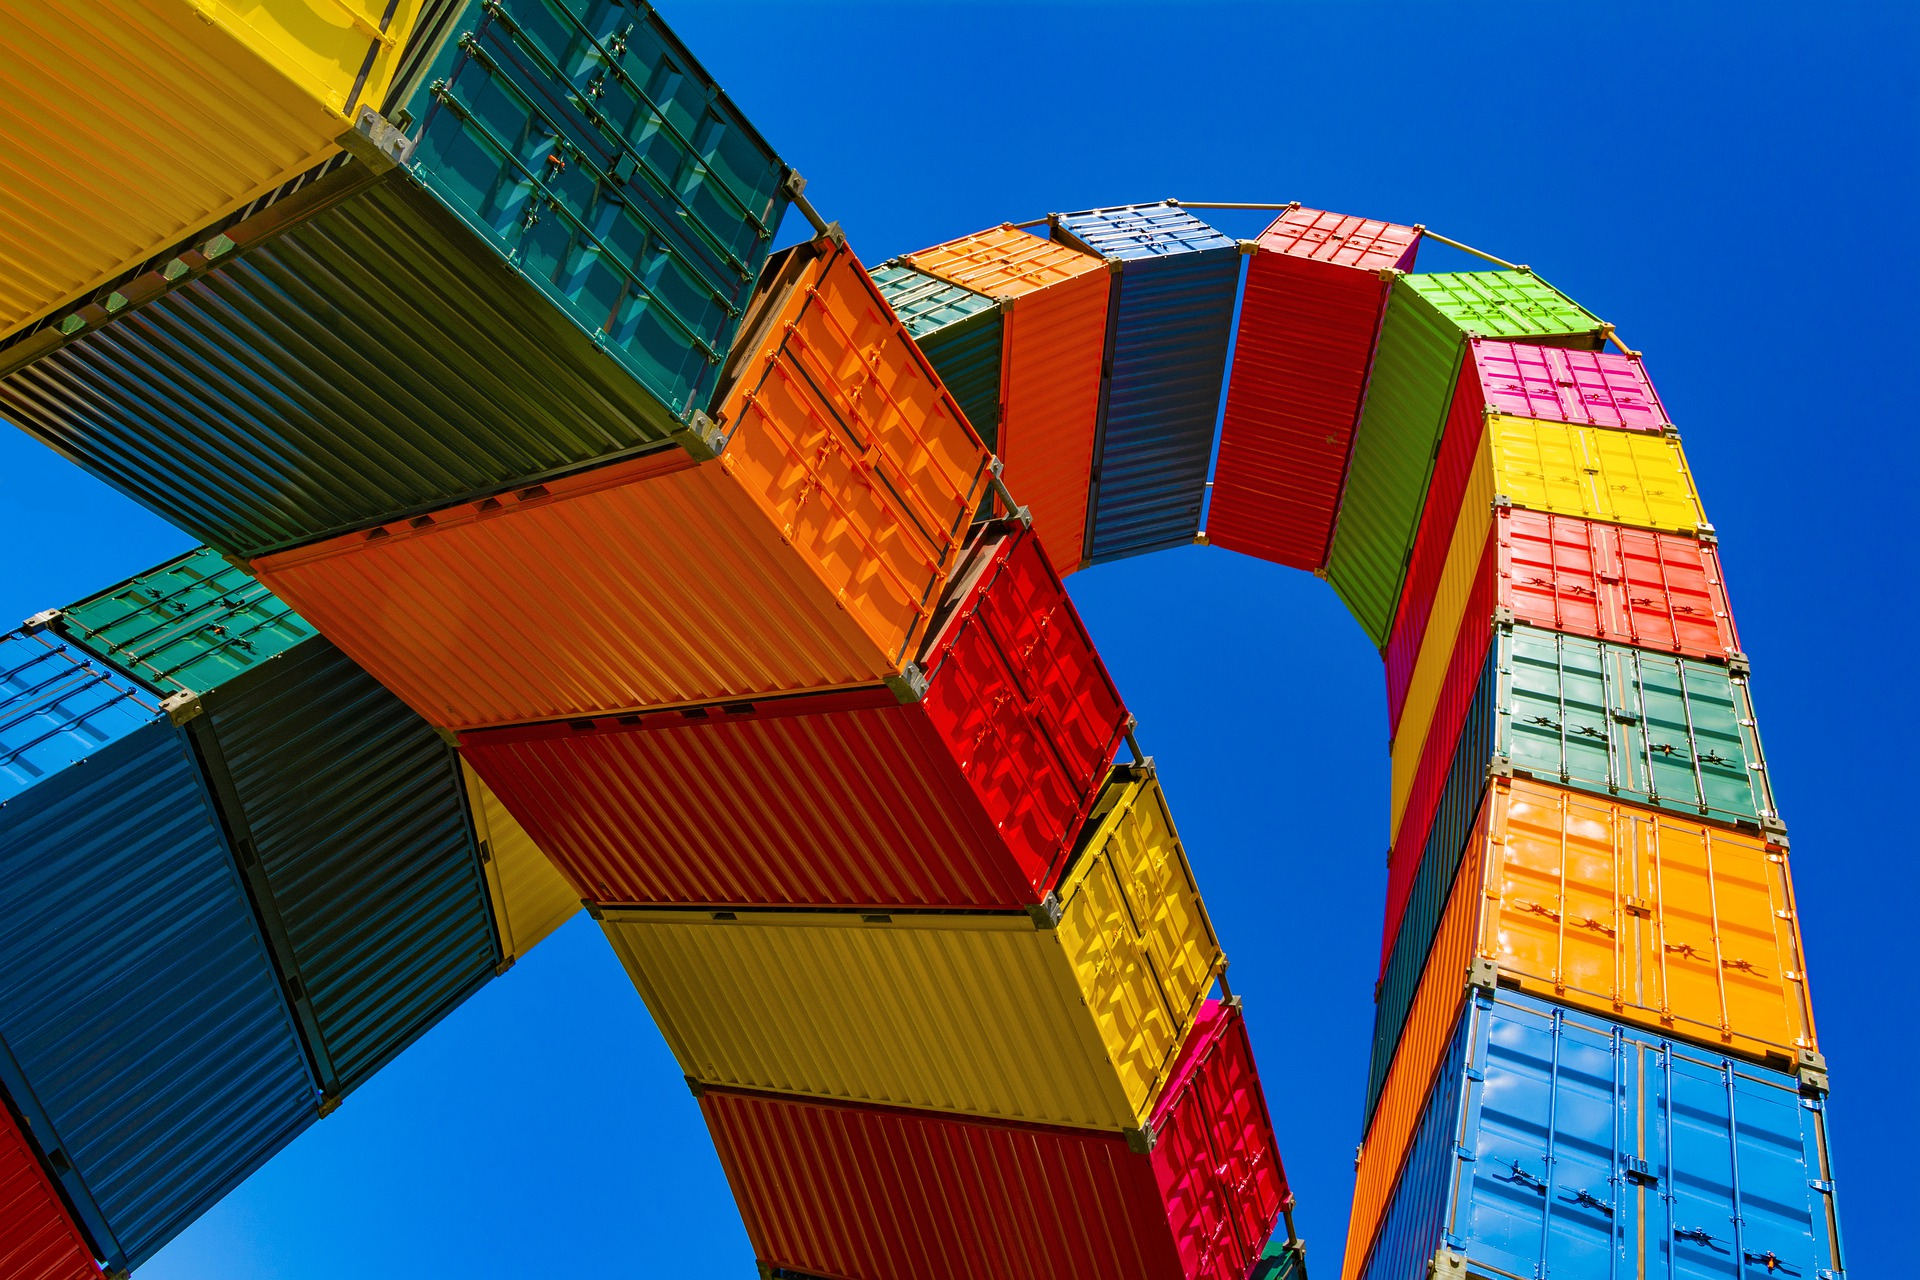
\includegraphics[scale=0.85]{21-docker.jpg}

\justifying
Containerization is the process of encapsulating the code and dependencies for part or all of a project. The most popular
and common tool for realizing containerization is Docker\index{Docker}. Using Docker, we can programatically build an
environment for our project, and pass the entirety of this encapsulated environment from our local
development machine, into the Continuous Integration (CI)\index{Continuous Integration} pipeline for testing, and eventually
into our production environment. Containerization\index{containerization} helps us by offering a consistent operating
experience across disparate environments.

\justifying
Recall our earlier discussion on the topics of immutability\index{immutability} and ephemerality\index{ephemerality}. It is more desirable
to create projects that are built and replaced frequently, than it is to attempt to upgrade and repair the infrastructure,
platforms, and project code on an on-going basis. Attempts to patch and upgrade project hosts ``in place'', quickly reveal
great difficulty in maintaining consistency with the project source, even when that source is stored in a revision control system.
These "in-place" upgrades and repairs may be the only option when it comes to certain software on ``bare metal'' hosts, and
hosts using certain virtualization technologies. A lesser degree of immutability
and ephemerality\index{ephemerality} also introduces issues keeping
operating system packages current, yet still compatible with the project. Imagine a situation where an upgrade to a package
is necessary to meet security requirements. What happens when this very same
upgrade means the project stops working since the package features that your application depends on have also changed?
The result is most likely angry end users and customers. Certainly not a situation we ever like to find ourselves in.

\section{Docker Containers}

\justifying
Docker images are ``canned'' (as in, prefabricated) or custom directives for provisioning a Docker container. One or more
images can be used as building blocks when configuring our containers. For example, a Linux image and Python image might
be combined with our customizations that describe and point to our application code, all of which make up a single container
that provides the functions of a fully provisioned server. We get the added
benefit of being able to switch quickly between base operating system images with just a few lines of code change to our
project. For example, we could easily modify our container image to be predicated on Debian
rather than Red Hat distribution of Linux kernel and operating system should the need arise.

\subsection{The .dockerignore File}

\section{Docker Hub}

\justifying
This is a repository for Docker containers. Many pre-built container images are available for download
from \href{https://hub.docker.com/}{Docker Hub}. You can also create an account and upload your own images from your various
projects.

\section{What is a Dockerfile?}

\justifying
The specification that outlines how a docker image is to be built is saved in the ``Dockerfile''.
The Dockerfile is our basic unit of containerization. That is to say, our containers, and the applications they contain, are defined by the
Dockerfile. This Dockerfile will dictate how we provision resources and include operating system essentials and packages inside our container. Each Dockerfile is predicated on a base image, such as ``python:slim-bullseye'' for example.

\justifying
One common technique to speed up our build pipelines is to simply pass along the Dockerfile, rather than
building and passing a container image along to others.

\justifying
\begin{mybox}{\thetcbcounter: Dockerfile}
  \lstinputlisting{code/21-docker/Dockerfile}
  \label{mydockerfile}
\end{mybox}

\justifying
A valid Dockerfile begins with the \textbf{FROM} instruction. This instruction specifies the base image that we
will use to build our project on. These base images come from the
\href{https://docs.docker.com/docker-hub/repos/}{Docker Hub repositories}. We are setting an environment variable
\textbf{DEBIAN\_FRONTEND} to the value of noninteractive, which will cause the apt command to skip or ignore any
interactive menus that are encountered during execution of the apt command, since these would cause
our builds to ``hang up'' at an inaccessible interactive prompt. The \textbf{ADD} and \textbf{WORKDIR} directives
are meant to cause Docker to use the /workdir directory as the root of the project ``inside'' the
container. Finally, we are directing Docker to \textbf{RUN} and apt update and install the apt-utils package.

\section{docker-compose.yml}
\justifying
The docker-compose tool and its associated docker-compose.yml file allows us to manage multiple Docker containers for
one or more applications in the same project. We will add this file to our project to illustrate it's
composition and give ourselves the ability to extend our work later, as needed.

\justifying
A file called docker-compose.yml\index{docker-compose.yml} will exist
alongside our Dockerfile in our docker directory.

\begin{mybox}{\thetcbcounter: Example docker-compose.yml}
  \lstinputlisting{code/21-docker/docker-compose.yml}
\end{mybox}

\justifying
The docker-compose.yml file begins with a version specification. It's important to note that the commands and structure
of docker-compose.yml can vary widely based on this version. While versions cannot be mixed, all version are valid with
respect to docker-compose itself. We specify a service named ``devsecops'', and assign a host and container name. Under
``volumes'' we are mounting the base of the project directory in the host
filesystem as ``/project'' in the container filesystem. The build
``directive'' tells docker-compose how to locate the Dockerfile we wish to use for the containers.

\justifying
With Docker properly installed and an understanding of the necessary configuration files, we can now do a bit of testing.
See the figure\ref{dockerdirectory} for an illustration of how to lay out the project files in your local file system.

\begin{figure}[!htb]
  \centering
  \chapter{Containers}

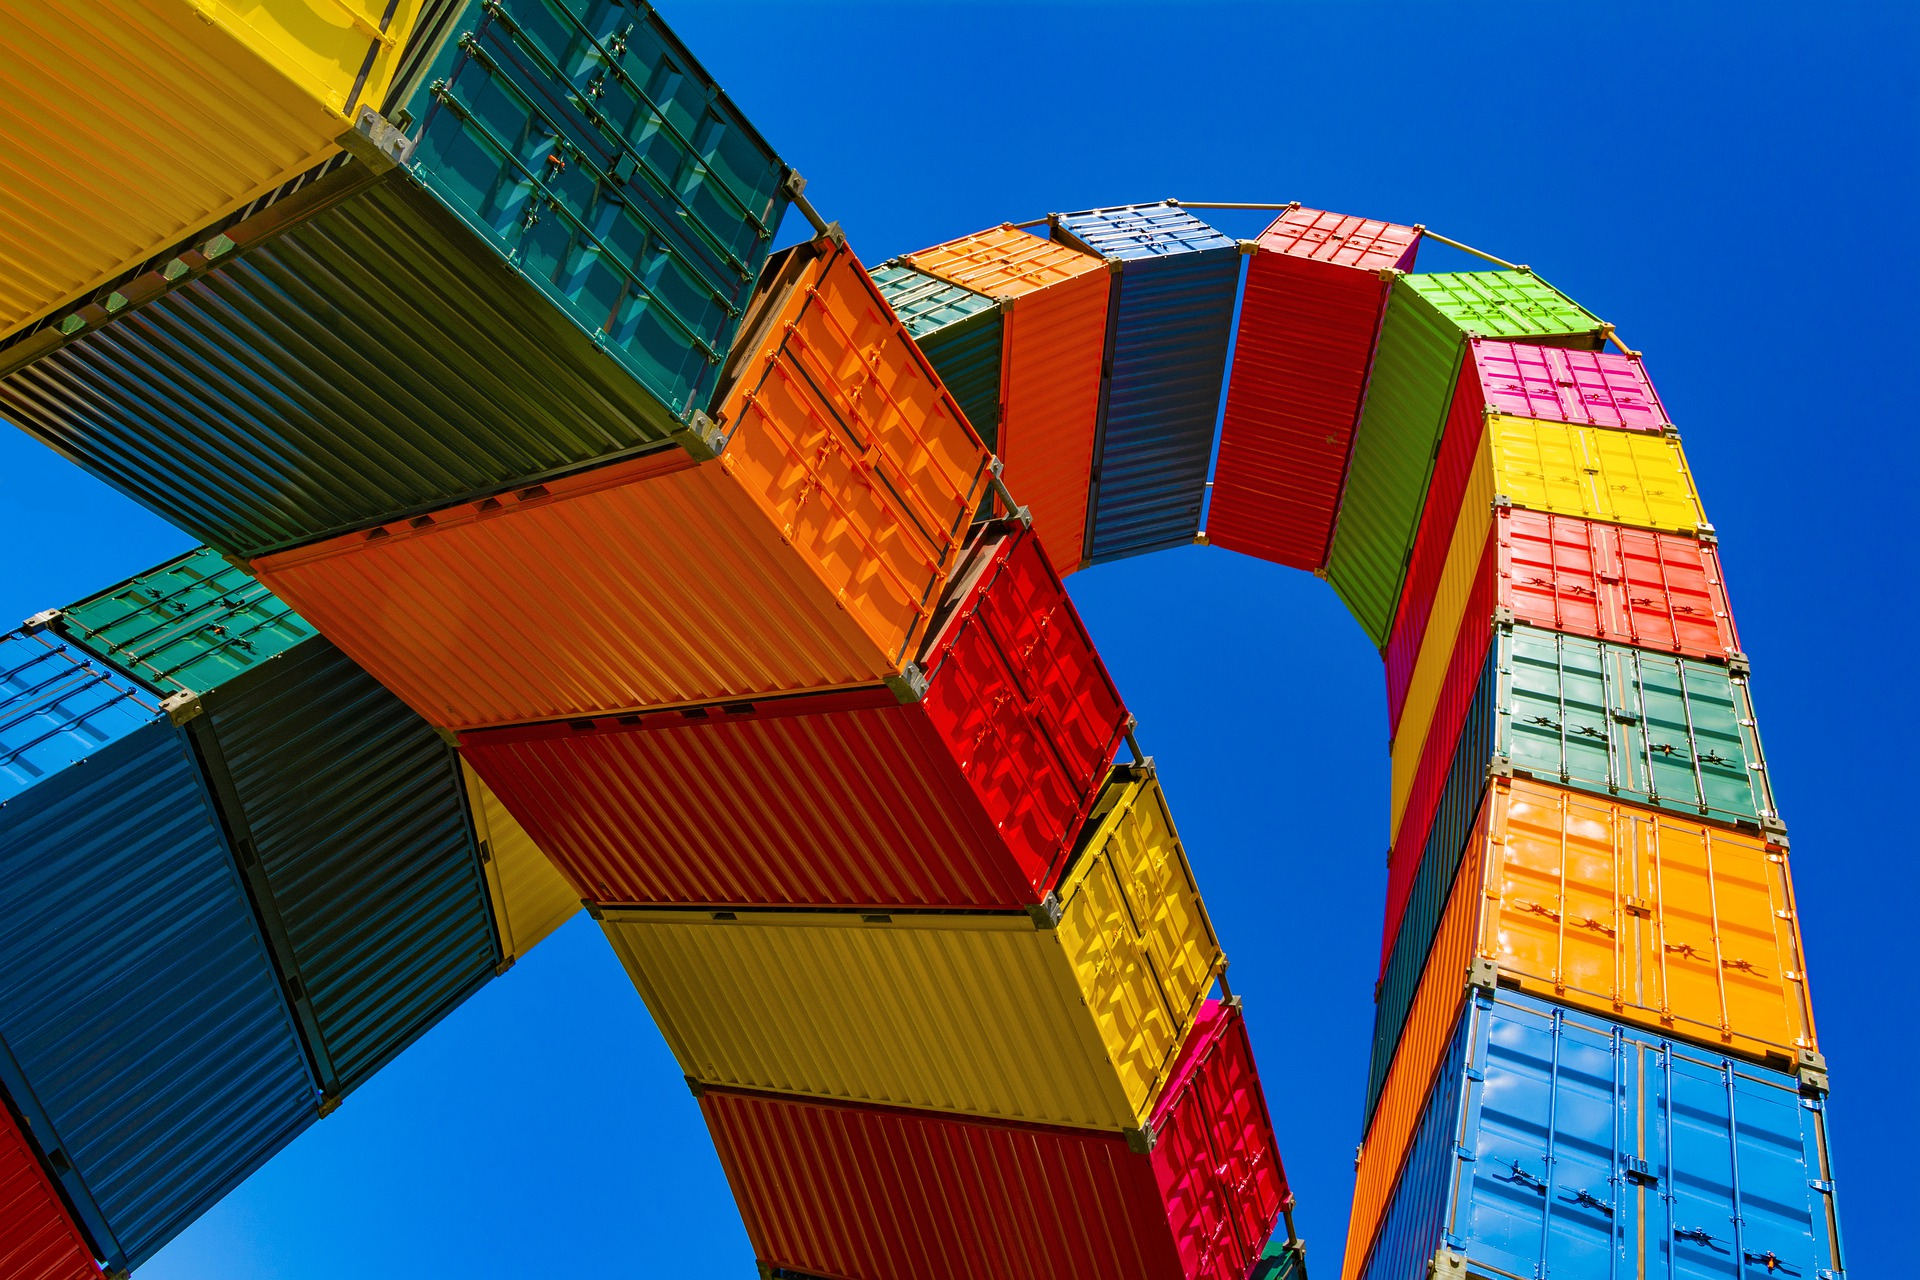
\includegraphics[scale=0.85]{21-docker.jpg}

\justifying
Containerization is the process of encapsulating the code and dependencies for part or all of a project. The most popular
and common tool for realizing containerization is Docker\index{Docker}. Using Docker, we can programatically build an
environment for our project, and pass the entirety of this encapsulated environment from our local
development machine, into the Continuous Integration (CI)\index{Continuous Integration} pipeline for testing, and eventually
into our production environment. Containerization\index{containerization} helps us by offering a consistent operating
experience across disparate environments.

\justifying
Recall our earlier discussion on the topics of immutability\index{immutability} and ephemerality\index{ephemerality}. It is more desirable
to create projects that are built and replaced frequently, than it is to attempt to upgrade and repair the infrastructure,
platforms, and project code on an on-going basis. Attempts to patch and upgrade project hosts ``in place'', quickly reveal
great difficulty in maintaining consistency with the project source, even when that source is stored in a revision control system.
These "in-place" upgrades and repairs may be the only option when it comes to certain software on ``bare metal'' hosts, and
hosts using certain virtualization technologies. A lesser degree of immutability
and ephemerality\index{ephemerality} also introduces issues keeping
operating system packages current, yet still compatible with the project. Imagine a situation where an upgrade to a package
is necessary to meet security requirements. What happens when this very same
upgrade means the project stops working since the package features that your application depends on have also changed?
The result is most likely angry end users and customers. Certainly not a situation we ever like to find ourselves in.

\section{Docker Containers}

\justifying
Docker images are ``canned'' (as in, prefabricated) or custom directives for provisioning a Docker container. One or more
images can be used as building blocks when configuring our containers. For example, a Linux image and Python image might
be combined with our customizations that describe and point to our application code, all of which make up a single container
that provides the functions of a fully provisioned server. We get the added
benefit of being able to switch quickly between base operating system images with just a few lines of code change to our
project. For example, we could easily modify our container image to be predicated on Debian
rather than Red Hat distribution of Linux kernel and operating system should the need arise.

\subsection{The .dockerignore File}

\section{Docker Hub}

\justifying
This is a repository for Docker containers. Many pre-built container images are available for download
from \href{https://hub.docker.com/}{Docker Hub}. You can also create an account and upload your own images from your various
projects.

\section{What is a Dockerfile?}

\justifying
The specification that outlines how a docker image is to be built is saved in the ``Dockerfile''.
The Dockerfile is our basic unit of containerization. That is to say, our containers, and the applications they contain, are defined by the
Dockerfile. This Dockerfile will dictate how we provision resources and include operating system essentials and packages inside our container. Each Dockerfile is predicated on a base image, such as ``python:slim-bullseye'' for example.

\justifying
One common technique to speed up our build pipelines is to simply pass along the Dockerfile, rather than
building and passing a container image along to others.

\justifying
\begin{mybox}{\thetcbcounter: Dockerfile}
  \lstinputlisting{code/21-docker/Dockerfile}
  \label{mydockerfile}
\end{mybox}

\justifying
A valid Dockerfile begins with the \textbf{FROM} instruction. This instruction specifies the base image that we
will use to build our project on. These base images come from the
\href{https://docs.docker.com/docker-hub/repos/}{Docker Hub repositories}. We are setting an environment variable
\textbf{DEBIAN\_FRONTEND} to the value of noninteractive, which will cause the apt command to skip or ignore any
interactive menus that are encountered during execution of the apt command, since these would cause
our builds to ``hang up'' at an inaccessible interactive prompt. The \textbf{ADD} and \textbf{WORKDIR} directives
are meant to cause Docker to use the /workdir directory as the root of the project ``inside'' the
container. Finally, we are directing Docker to \textbf{RUN} and apt update and install the apt-utils package.

\section{docker-compose.yml}
\justifying
The docker-compose tool and its associated docker-compose.yml file allows us to manage multiple Docker containers for
one or more applications in the same project. We will add this file to our project to illustrate it's
composition and give ourselves the ability to extend our work later, as needed.

\justifying
A file called docker-compose.yml\index{docker-compose.yml} will exist
alongside our Dockerfile in our docker directory.

\begin{mybox}{\thetcbcounter: Example docker-compose.yml}
  \lstinputlisting{code/21-docker/docker-compose.yml}
\end{mybox}

\justifying
The docker-compose.yml file begins with a version specification. It's important to note that the commands and structure
of docker-compose.yml can vary widely based on this version. While versions cannot be mixed, all version are valid with
respect to docker-compose itself. We specify a service named ``devsecops'', and assign a host and container name. Under
``volumes'' we are mounting the base of the project directory in the host
filesystem as ``/project'' in the container filesystem. The build
``directive'' tells docker-compose how to locate the Dockerfile we wish to use for the containers.

\justifying
With Docker properly installed and an understanding of the necessary configuration files, we can now do a bit of testing.
See the figure\ref{dockerdirectory} for an illustration of how to lay out the project files in your local file system.

\begin{figure}[!htb]
  \centering
  \chapter{Containers}

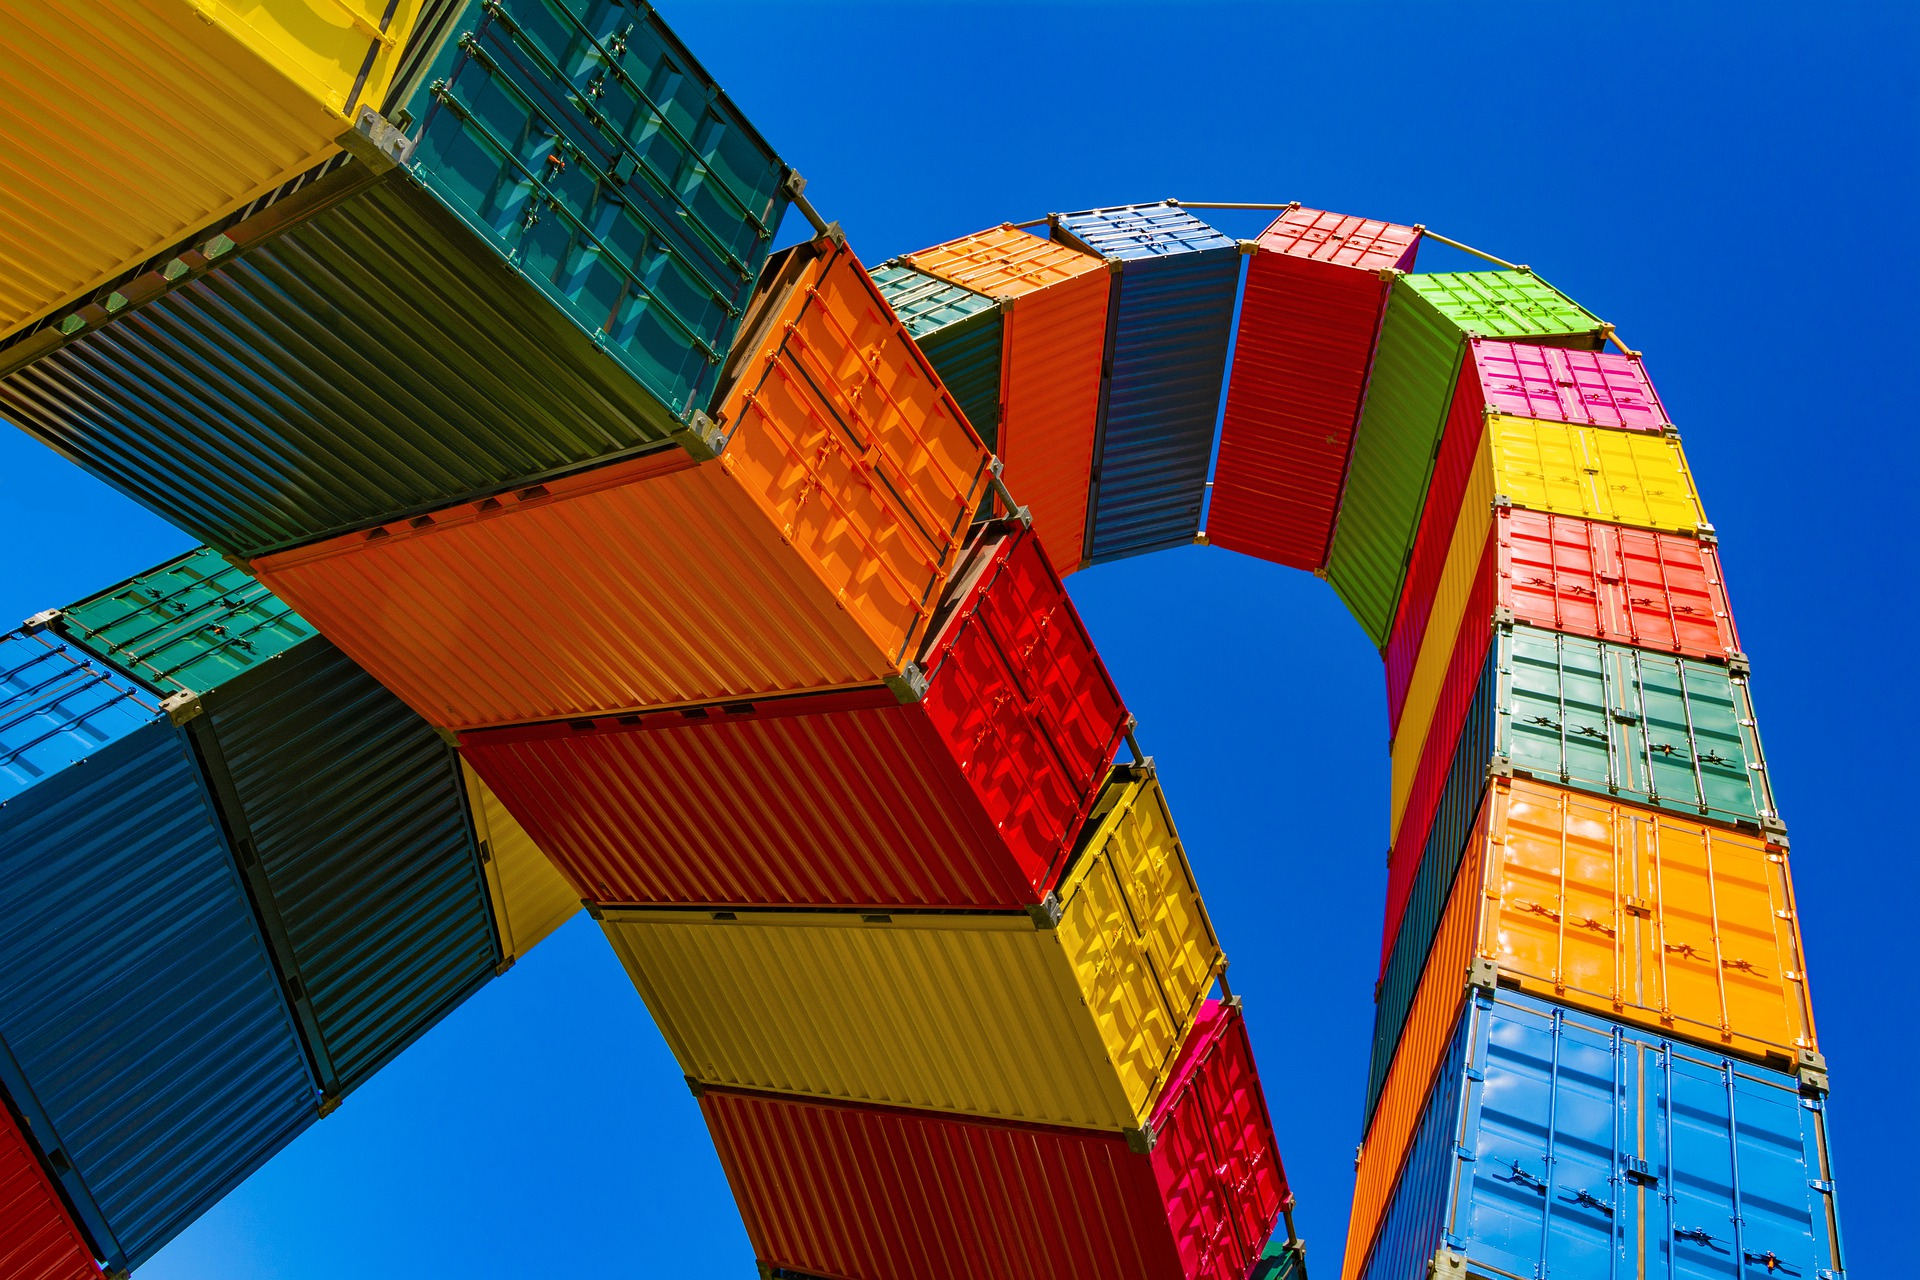
\includegraphics[scale=0.85]{21-docker.jpg}

\justifying
Containerization is the process of encapsulating the code and dependencies for part or all of a project. The most popular
and common tool for realizing containerization is Docker\index{Docker}. Using Docker, we can programatically build an
environment for our project, and pass the entirety of this encapsulated environment from our local
development machine, into the Continuous Integration (CI)\index{Continuous Integration} pipeline for testing, and eventually
into our production environment. Containerization\index{containerization} helps us by offering a consistent operating
experience across disparate environments.

\justifying
Recall our earlier discussion on the topics of immutability\index{immutability} and ephemerality\index{ephemerality}. It is more desirable
to create projects that are built and replaced frequently, than it is to attempt to upgrade and repair the infrastructure,
platforms, and project code on an on-going basis. Attempts to patch and upgrade project hosts ``in place'', quickly reveal
great difficulty in maintaining consistency with the project source, even when that source is stored in a revision control system.
These "in-place" upgrades and repairs may be the only option when it comes to certain software on ``bare metal'' hosts, and
hosts using certain virtualization technologies. A lesser degree of immutability
and ephemerality\index{ephemerality} also introduces issues keeping
operating system packages current, yet still compatible with the project. Imagine a situation where an upgrade to a package
is necessary to meet security requirements. What happens when this very same
upgrade means the project stops working since the package features that your application depends on have also changed?
The result is most likely angry end users and customers. Certainly not a situation we ever like to find ourselves in.

\section{Docker Containers}

\justifying
Docker images are ``canned'' (as in, prefabricated) or custom directives for provisioning a Docker container. One or more
images can be used as building blocks when configuring our containers. For example, a Linux image and Python image might
be combined with our customizations that describe and point to our application code, all of which make up a single container
that provides the functions of a fully provisioned server. We get the added
benefit of being able to switch quickly between base operating system images with just a few lines of code change to our
project. For example, we could easily modify our container image to be predicated on Debian
rather than Red Hat distribution of Linux kernel and operating system should the need arise.

\subsection{The .dockerignore File}

\section{Docker Hub}

\justifying
This is a repository for Docker containers. Many pre-built container images are available for download
from \href{https://hub.docker.com/}{Docker Hub}. You can also create an account and upload your own images from your various
projects.

\section{What is a Dockerfile?}

\justifying
The specification that outlines how a docker image is to be built is saved in the ``Dockerfile''.
The Dockerfile is our basic unit of containerization. That is to say, our containers, and the applications they contain, are defined by the
Dockerfile. This Dockerfile will dictate how we provision resources and include operating system essentials and packages inside our container. Each Dockerfile is predicated on a base image, such as ``python:slim-bullseye'' for example.

\justifying
One common technique to speed up our build pipelines is to simply pass along the Dockerfile, rather than
building and passing a container image along to others.

\justifying
\begin{mybox}{\thetcbcounter: Dockerfile}
  \lstinputlisting{code/21-docker/Dockerfile}
  \label{mydockerfile}
\end{mybox}

\justifying
A valid Dockerfile begins with the \textbf{FROM} instruction. This instruction specifies the base image that we
will use to build our project on. These base images come from the
\href{https://docs.docker.com/docker-hub/repos/}{Docker Hub repositories}. We are setting an environment variable
\textbf{DEBIAN\_FRONTEND} to the value of noninteractive, which will cause the apt command to skip or ignore any
interactive menus that are encountered during execution of the apt command, since these would cause
our builds to ``hang up'' at an inaccessible interactive prompt. The \textbf{ADD} and \textbf{WORKDIR} directives
are meant to cause Docker to use the /workdir directory as the root of the project ``inside'' the
container. Finally, we are directing Docker to \textbf{RUN} and apt update and install the apt-utils package.

\section{docker-compose.yml}
\justifying
The docker-compose tool and its associated docker-compose.yml file allows us to manage multiple Docker containers for
one or more applications in the same project. We will add this file to our project to illustrate it's
composition and give ourselves the ability to extend our work later, as needed.

\justifying
A file called docker-compose.yml\index{docker-compose.yml} will exist
alongside our Dockerfile in our docker directory.

\begin{mybox}{\thetcbcounter: Example docker-compose.yml}
  \lstinputlisting{code/21-docker/docker-compose.yml}
\end{mybox}

\justifying
The docker-compose.yml file begins with a version specification. It's important to note that the commands and structure
of docker-compose.yml can vary widely based on this version. While versions cannot be mixed, all version are valid with
respect to docker-compose itself. We specify a service named ``devsecops'', and assign a host and container name. Under
``volumes'' we are mounting the base of the project directory in the host
filesystem as ``/project'' in the container filesystem. The build
``directive'' tells docker-compose how to locate the Dockerfile we wish to use for the containers.

\justifying
With Docker properly installed and an understanding of the necessary configuration files, we can now do a bit of testing.
See the figure\ref{dockerdirectory} for an illustration of how to lay out the project files in your local file system.

\begin{figure}[!htb]
  \centering
  \input{dot/21-docker.tex}
  \caption{Project Directory and Docker related files.}
\label{dockerdirectory}
\end{figure}

\markdownInput{../labs/ch4/lab-4a.md}

\justifying
In later chapters we will explore how to ``clone'' a project repository from \href{github.com} and do our work directory
from there. It is a good practice to keep a Dockerfile at the top level of your GitHub repository that can be used to
build and test your application.

\markdownInput{../labs/ch4/lab-4b.md}

\justifying
\begin{mybox}{\thetcbcounter: Dockerfile.fixed}
    \lstinputlisting{code/21-docker/Dockerfile.fixed}
    \label{fixeddockerfile}
\end{mybox}

\markdownInput{../labs/ch4/lab-4c.md}

% https://www.paloaltonetworks.com/cyberpedia/what-is-container-security

%\section{Podman and Buildah}

%\justifying
%Note that Podman\index{Podman} is an acceptable substitute for Docker.
%Podman is an Open Source tool from the Open Containers Initiative (OCI)\index{Open Containers Initiative
%(OCI)}. The Podman\index{Podman} service is said to be capable of being a drop-in replacement for Docker, although it only runs on Linux hosts at the time of this writing. Podman gives
%the user the ability to use traditional Docker commands,
%without the need to run a daemon to do so\cite{podman}, as is the case with Docker.

%\justifying
%You can install Podman by
%\href{https://podman.io/getting-started/installation.html}{following the instructions}
%at their website. Once Podman is installed properly you should be able to alias docker=podman and use it as a
%drop-in replacement for Docker and it's associated daemon.

\section{Volumes}

It is often desirable to write files between the host system and a running Docker container. We can accomplish this by taking advantage of the Docker concept of ``Volumes''. This is \href{https://docs.docker.com/storage/volumes/#use-a-volume-with-docker-compose}{easy to achieve thanks to docker-compose}.

\markdownInput{../labs/ch4/lab-4d.md}

\justifying
With this lab we are able to illustrate the concept of mounting a volume to be shared between our host system and a
container image. The ability to write files between the two environments means we can quickly spin up a small container and have an
encapsulated ``scratch workspace'' with minimal effort. Often I will use this pattern to try our different dependencies, say
different versions of a Python module to see how it will interact (or if I can get things to build at all!). The host machine is
not cluttered with packages, dependencies, and failed attempts at building and configuring things at the end of the working
session.

\justifying
Another interesting result is that we can create files and directories on the host without the usual (albiet minor) annoyance
that they will all be owned by the superuser.

\section{Container Orchestration}

\justifying
An orchestrator for containers can be thought of as an engine which allows for their provisioning, deployment, scaling, monitoring, load
balancing, and more. The Container Orchestrator manages the life cycle and visibility of a container at all stages.

\justifying
Kubernetes\index{Kubernetes} is an example, perhaps even the penultimate example, of a Container Orchestrator\index{orchestration}.
Folks throughout the DevSecOps, Software and Security communities are using Kubernetes these days, and
with good reason. It's adoption as a means to manage and replicate containers, and scale the applications they contain,
has been nothing short of revolutionary. System administrators and developers can do more, better work. Granted, this comes at
the expense of introduction yet another framework to learn, and no small amount of complexity.

\justifying
An orchestrator helps us achieve immutability, and scale to meet user demand quickly and easily by abstracting away
concerns that come with operating workloads in a bare metal or VM environment.

\justifying
Kubernetes and other orchestrators are rapidly evolving. To ignore this game-changing ecosystem is to be left behind in terms of technological prowess. Learning about containers, pipelines, infrastructure, and
so on are the foundational elements you will want to become familiar with in preparation for expanding your mindset into the greater
dimensionality that orchestration realizes.

\justifying
Later we will look more closely at the sprawling and vibrant topic of Kubernetes \index{Kubernetes}. For this stage of our journey to DevSecOps
enlightenment, it is enough to know that orchestration exists and have a bit of familiarity with its purpose.

  \caption{Project Directory and Docker related files.}
\label{dockerdirectory}
\end{figure}

\markdownInput{../labs/ch4/lab-4a.md}

\justifying
In later chapters we will explore how to ``clone'' a project repository from \href{github.com} and do our work directory
from there. It is a good practice to keep a Dockerfile at the top level of your GitHub repository that can be used to
build and test your application.

\markdownInput{../labs/ch4/lab-4b.md}

\justifying
\begin{mybox}{\thetcbcounter: Dockerfile.fixed}
    \lstinputlisting{code/21-docker/Dockerfile.fixed}
    \label{fixeddockerfile}
\end{mybox}

\markdownInput{../labs/ch4/lab-4c.md}

% https://www.paloaltonetworks.com/cyberpedia/what-is-container-security

%\section{Podman and Buildah}

%\justifying
%Note that Podman\index{Podman} is an acceptable substitute for Docker.
%Podman is an Open Source tool from the Open Containers Initiative (OCI)\index{Open Containers Initiative
%(OCI)}. The Podman\index{Podman} service is said to be capable of being a drop-in replacement for Docker, although it only runs on Linux hosts at the time of this writing. Podman gives
%the user the ability to use traditional Docker commands,
%without the need to run a daemon to do so\cite{podman}, as is the case with Docker.

%\justifying
%You can install Podman by
%\href{https://podman.io/getting-started/installation.html}{following the instructions}
%at their website. Once Podman is installed properly you should be able to alias docker=podman and use it as a
%drop-in replacement for Docker and it's associated daemon.

\section{Volumes}

It is often desirable to write files between the host system and a running Docker container. We can accomplish this by taking advantage of the Docker concept of ``Volumes''. This is \href{https://docs.docker.com/storage/volumes/#use-a-volume-with-docker-compose}{easy to achieve thanks to docker-compose}.

\markdownInput{../labs/ch4/lab-4d.md}

\justifying
With this lab we are able to illustrate the concept of mounting a volume to be shared between our host system and a
container image. The ability to write files between the two environments means we can quickly spin up a small container and have an
encapsulated ``scratch workspace'' with minimal effort. Often I will use this pattern to try our different dependencies, say
different versions of a Python module to see how it will interact (or if I can get things to build at all!). The host machine is
not cluttered with packages, dependencies, and failed attempts at building and configuring things at the end of the working
session.

\justifying
Another interesting result is that we can create files and directories on the host without the usual (albiet minor) annoyance
that they will all be owned by the superuser.

\section{Container Orchestration}

\justifying
An orchestrator for containers can be thought of as an engine which allows for their provisioning, deployment, scaling, monitoring, load
balancing, and more. The Container Orchestrator manages the life cycle and visibility of a container at all stages.

\justifying
Kubernetes\index{Kubernetes} is an example, perhaps even the penultimate example, of a Container Orchestrator\index{orchestration}.
Folks throughout the DevSecOps, Software and Security communities are using Kubernetes these days, and
with good reason. It's adoption as a means to manage and replicate containers, and scale the applications they contain,
has been nothing short of revolutionary. System administrators and developers can do more, better work. Granted, this comes at
the expense of introduction yet another framework to learn, and no small amount of complexity.

\justifying
An orchestrator helps us achieve immutability, and scale to meet user demand quickly and easily by abstracting away
concerns that come with operating workloads in a bare metal or VM environment.

\justifying
Kubernetes and other orchestrators are rapidly evolving. To ignore this game-changing ecosystem is to be left behind in terms of technological prowess. Learning about containers, pipelines, infrastructure, and
so on are the foundational elements you will want to become familiar with in preparation for expanding your mindset into the greater
dimensionality that orchestration realizes.

\justifying
Later we will look more closely at the sprawling and vibrant topic of Kubernetes \index{Kubernetes}. For this stage of our journey to DevSecOps
enlightenment, it is enough to know that orchestration exists and have a bit of familiarity with its purpose.

  \caption{Project Directory and Docker related files.}
\label{dockerdirectory}
\end{figure}

\markdownInput{../labs/ch4/lab-4a.md}

\justifying
In later chapters we will explore how to ``clone'' a project repository from \href{github.com} and do our work directory
from there. It is a good practice to keep a Dockerfile at the top level of your GitHub repository that can be used to
build and test your application.

\markdownInput{../labs/ch4/lab-4b.md}

\justifying
\begin{mybox}{\thetcbcounter: Dockerfile.fixed}
    \lstinputlisting{code/21-docker/Dockerfile.fixed}
    \label{fixeddockerfile}
\end{mybox}

\markdownInput{../labs/ch4/lab-4c.md}

% https://www.paloaltonetworks.com/cyberpedia/what-is-container-security

%\section{Podman and Buildah}

%\justifying
%Note that Podman\index{Podman} is an acceptable substitute for Docker.
%Podman is an Open Source tool from the Open Containers Initiative (OCI)\index{Open Containers Initiative
%(OCI)}. The Podman\index{Podman} service is said to be capable of being a drop-in replacement for Docker, although it only runs on Linux hosts at the time of this writing. Podman gives
%the user the ability to use traditional Docker commands,
%without the need to run a daemon to do so\cite{podman}, as is the case with Docker.

%\justifying
%You can install Podman by
%\href{https://podman.io/getting-started/installation.html}{following the instructions}
%at their website. Once Podman is installed properly you should be able to alias docker=podman and use it as a
%drop-in replacement for Docker and it's associated daemon.

\section{Volumes}

It is often desirable to write files between the host system and a running Docker container. We can accomplish this by taking advantage of the Docker concept of ``Volumes''. This is \href{https://docs.docker.com/storage/volumes/#use-a-volume-with-docker-compose}{easy to achieve thanks to docker-compose}.

\markdownInput{../labs/ch4/lab-4d.md}

\justifying
With this lab we are able to illustrate the concept of mounting a volume to be shared between our host system and a
container image. The ability to write files between the two environments means we can quickly spin up a small container and have an
encapsulated ``scratch workspace'' with minimal effort. Often I will use this pattern to try our different dependencies, say
different versions of a Python module to see how it will interact (or if I can get things to build at all!). The host machine is
not cluttered with packages, dependencies, and failed attempts at building and configuring things at the end of the working
session.

\justifying
Another interesting result is that we can create files and directories on the host without the usual (albiet minor) annoyance
that they will all be owned by the superuser.

\section{Container Orchestration}

\justifying
An orchestrator for containers can be thought of as an engine which allows for their provisioning, deployment, scaling, monitoring, load
balancing, and more. The Container Orchestrator manages the life cycle and visibility of a container at all stages.

\justifying
Kubernetes\index{Kubernetes} is an example, perhaps even the penultimate example, of a Container Orchestrator\index{orchestration}.
Folks throughout the DevSecOps, Software and Security communities are using Kubernetes these days, and
with good reason. It's adoption as a means to manage and replicate containers, and scale the applications they contain,
has been nothing short of revolutionary. System administrators and developers can do more, better work. Granted, this comes at
the expense of introduction yet another framework to learn, and no small amount of complexity.

\justifying
An orchestrator helps us achieve immutability, and scale to meet user demand quickly and easily by abstracting away
concerns that come with operating workloads in a bare metal or VM environment.

\justifying
Kubernetes and other orchestrators are rapidly evolving. To ignore this game-changing ecosystem is to be left behind in terms of technological prowess. Learning about containers, pipelines, infrastructure, and
so on are the foundational elements you will want to become familiar with in preparation for expanding your mindset into the greater
dimensionality that orchestration realizes.

\justifying
Later we will look more closely at the sprawling and vibrant topic of Kubernetes \index{Kubernetes}. For this stage of our journey to DevSecOps
enlightenment, it is enough to know that orchestration exists and have a bit of familiarity with its purpose.

\chapter{Revision Control}
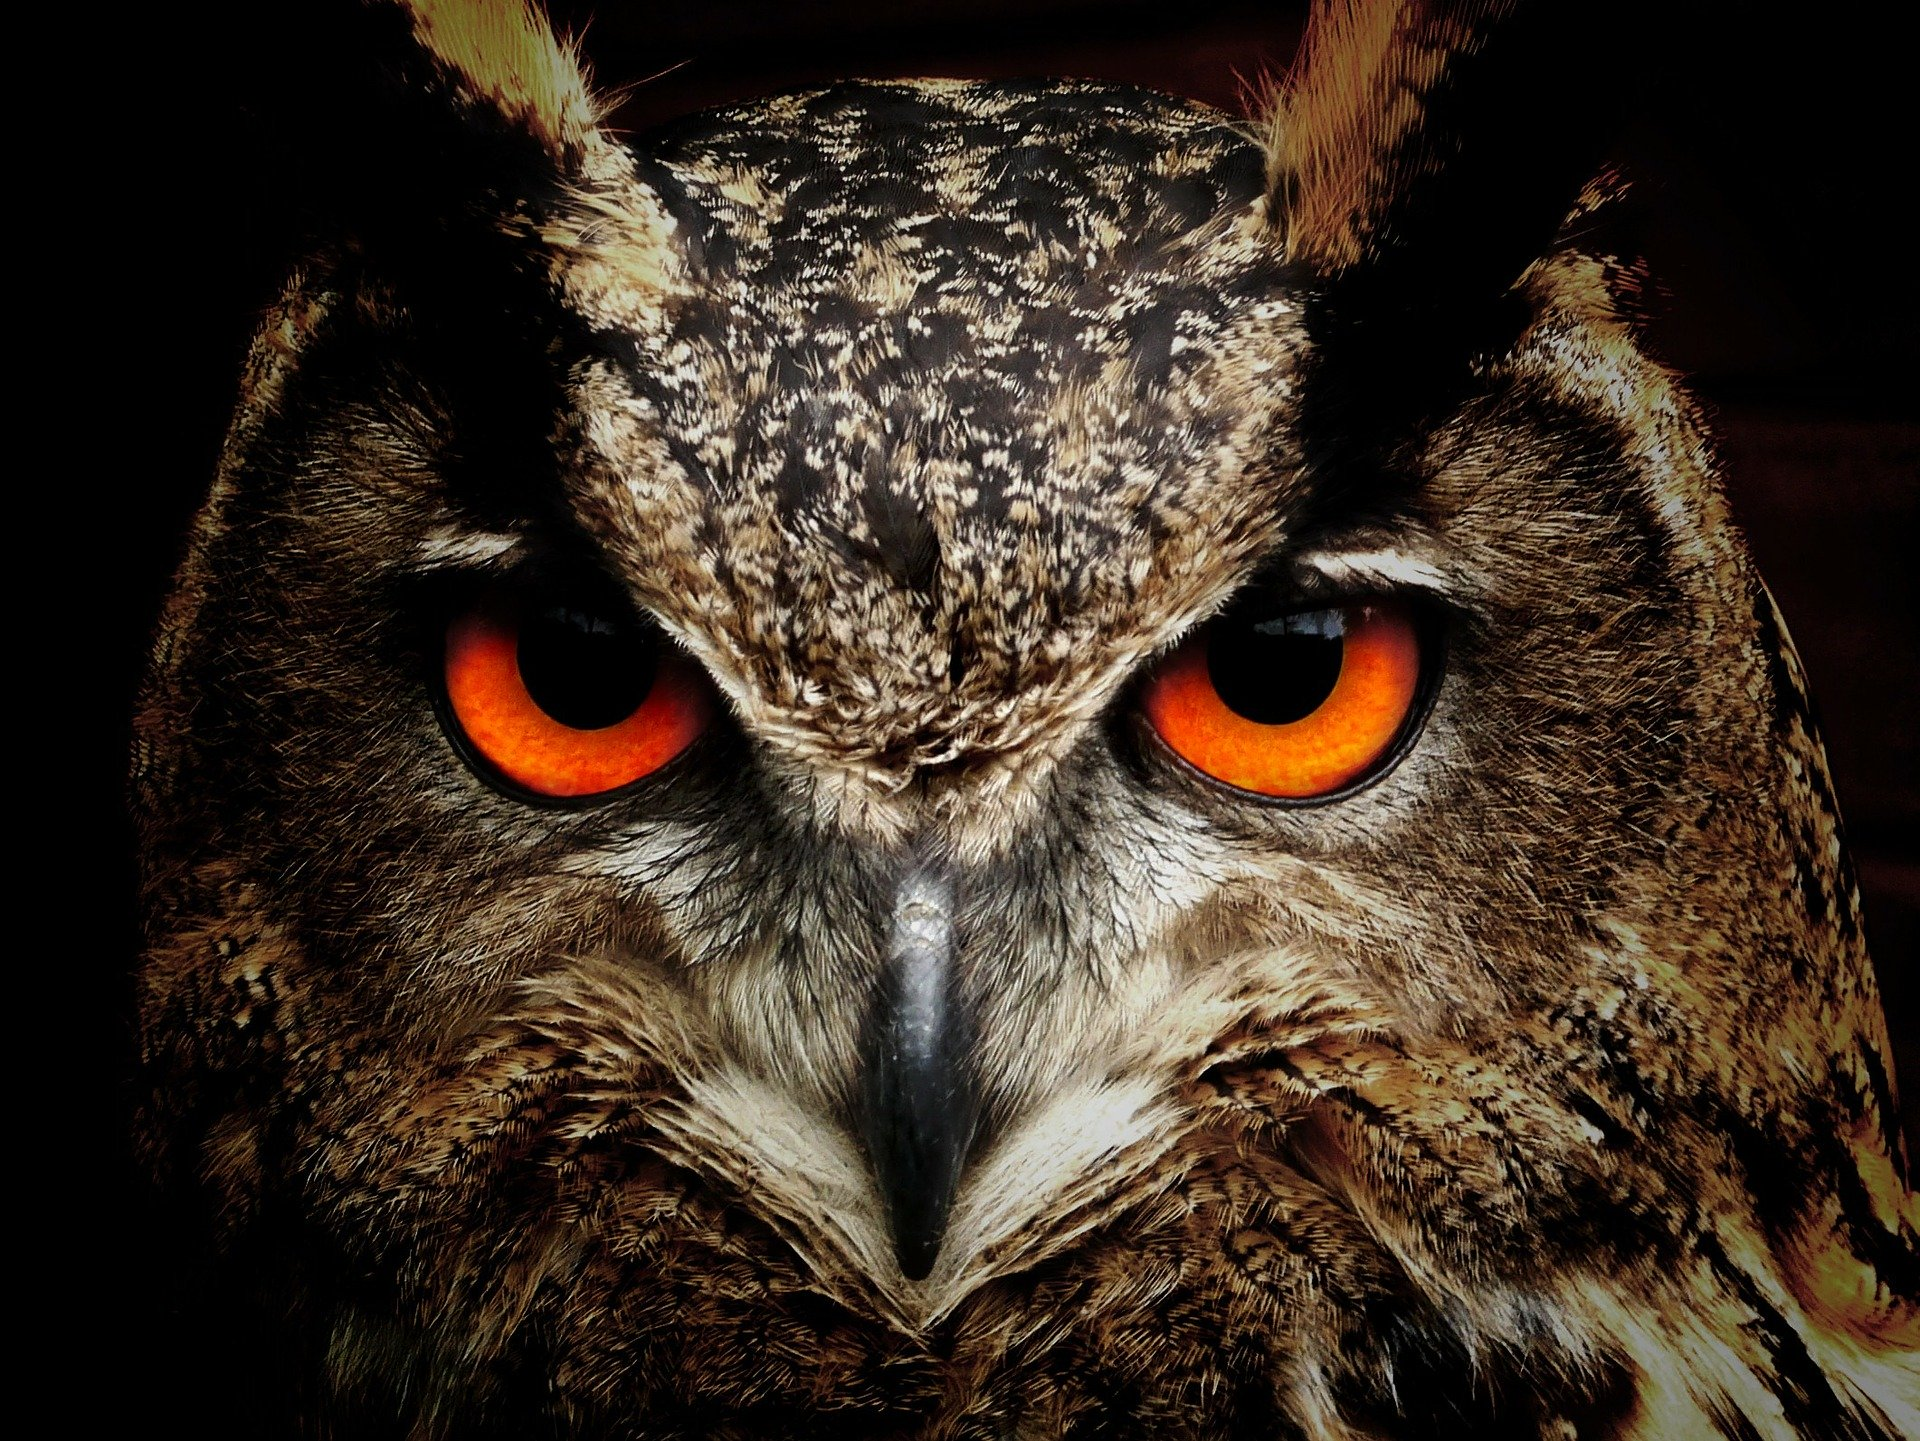
\includegraphics[scale=0.20]{images/owl-50267_1920.jpg}

\justifying
Using a revision control\index{revision control} methodology allows us to organize and store project artifacts. Typically these
artifacts are source code files but may include documentation, files to assist us with Kubernetes cluster management and application
deployment, and more. Websites like \href{https://github.com}{github.com} for example, are the modern
backbone of revision control, and foundational to our workflow. They are a key piece of our software delivery pipeline,
allowing us to declare a single source of truth for the code that makes up our project. Multiple users or teams can collaborate on a
single code base stored in a repository, the structure which encompasses a typical project. Even after the benefits from collaboration and
storage are considered, we can still realize a great benefit from being able to create releases, which can be tagged and ``rolled''
forward to and back from.

\justifying
There are other similar services we can choose from. These tend to be free for personal projects, non-commercial, and even some commercial
uses. For example \href{https://bitbucket.org/product}{Bitbucket} and \href{https://about.gitlab.com/}{GitLab}. For the purposes of this
book we will focus GitHub\index{GitHub}, since many people are familiar with it.

\justifying
Git is the tool that allows for revision control of your work. GitHub is a repository for storing that work, creating
teams to work on projects, tracking issues, defining release packages, and more. Simply put, \href{github.com}{github.com}
is a website that gives you a place to store the work you are using git to manage. Git was created in 2005 by
Linus Torvalds\index{Linus Torvalds}, who, as you may know, also created the Linux kernel.

\justifying
After creating your account on GitHub, one of the very first things you should do is to configure two-factor authentication (2FA)\index{2FA} for your GitHub account.
See \href{https://docs.github.com/en/github/authenticating-to-github/securing-your-account-with-two-factor-authentication-2fa}{securing your account with two factor authentication}
for more information. If you already have an account at GitHub, now is a good time to make sure you have this feature enabled. Two-factor authentication provides
an additional layer of security on your Github account, and is all-around good practice. Using two- or multi-factor authentication with a
password manager will do wonders
to improve your security hygiene. You may also use your password manager to store your account recovery codes. Creating a text file
that contains your recovery codes and keeping an encrypted copy in your home directory is another option.

\section{Creating a Repository}

Repository creation is well documented, for example
\href{https://docs.github.com/en/get-started/quickstart/create-a-repo}{these steps in the GitHub quick start pages}. Let look a bit
more closely ar what is involved in this process.

\justifying
Often I will start a new repository on my personal account while I use the steps in this book to get the project off the ground.
Later I will move the repository into an organization where the responsibility for ownership and administration can be
shared with other folks.

\justifying
Directions for the labs in this chapter are located in GitHub, of course!
\href{https://github.com/devsecfranklin/devsecops-tactical-workbook/tree/main/code/ch5}{Follow this link to view the lab files},
or simply proceed with the steps below.

\justifying
So far we have created the files seen in figure \ref{projfiles} to our project. There is much to be gained from bringing our project under revision control so let's
make that our next task. Take note, the ``top level'' for our GitHub repository will be the ``myproject'' folder even though we have some files in our ``/home/devsecops''
home directory that impact our project. We want to keep a separation between the source code and documentation in the ``myproject'' folder and any machine specific
configuration that is present on an individual developers workstation.

\begin{figure}[!htb]
\centering

\begin{tikzpicture}[>=latex,line join=bevel,]
  \pgfsetlinewidth{1bp}
%%
\pgfsetcolor{black}
  % Edge: framework -> pass
  \draw [->] (176.55bp,215.88bp) .. controls (156.36bp,206.39bp) and (131.08bp,194.51bp)  .. (100.33bp,180.07bp);
  % Edge: framework -> gnupg
  \draw [->] (203.36bp,215.7bp) .. controls (198.87bp,207.64bp) and (193.44bp,197.89bp)  .. (183.53bp,180.1bp);
  % Edge: framework -> docker
  \draw [->] (222.64bp,215.7bp) .. controls (227.13bp,207.64bp) and (232.56bp,197.89bp)  .. (242.47bp,180.1bp);
  % Edge: framework -> workspace
  \draw [->] (245.29bp,215.88bp) .. controls (262.87bp,206.55bp) and (284.81bp,194.92bp)  .. (312.59bp,180.19bp);
  % Edge: workspace -> myproject
  \draw [->] (345.0bp,143.7bp) .. controls (345.0bp,135.98bp) and (345.0bp,126.71bp)  .. (345.0bp,108.1bp);
  % Edge: myproject -> dockercom
  \draw [->] (328.19bp,71.697bp) .. controls (319.87bp,63.135bp) and (309.69bp,52.656bp)  .. (293.62bp,36.104bp);
  % Edge: myproject -> Dockerfile
  \draw [->] (361.81bp,71.697bp) .. controls (370.13bp,63.135bp) and (380.31bp,52.656bp)  .. (396.38bp,36.104bp);
  % Node: framework
\begin{scope}
  \definecolor{strokecol}{rgb}{0.0,0.0,0.0};
  \pgfsetstrokecolor{strokecol}
  \draw (274.0bp,252.0bp) -- (271.0bp,256.0bp) -- (250.0bp,256.0bp) -- (247.0bp,252.0bp) -- (152.0bp,252.0bp) -- (152.0bp,216.0bp) -- (274.0bp,216.0bp) -- cycle;
  \draw (213.0bp,234.0bp) node {/home/devsecops};
\end{scope}
  % Node: pass
\begin{scope}
  \definecolor{strokecol}{rgb}{0.0,0.0,0.0};
  \pgfsetstrokecolor{strokecol}
  \draw (128.0bp,180.0bp) -- (125.0bp,184.0bp) -- (104.0bp,184.0bp) -- (101.0bp,180.0bp) -- (0.0bp,180.0bp) -- (0.0bp,144.0bp) -- (128.0bp,144.0bp) -- cycle;
  \draw (64.0bp,162.0bp) node {.password-store};
\end{scope}
  % Node: gnupg
\begin{scope}
  \definecolor{strokecol}{rgb}{0.0,0.0,0.0};
  \pgfsetstrokecolor{strokecol}
  \draw (202.0bp,180.0bp) -- (199.0bp,184.0bp) -- (178.0bp,184.0bp) -- (175.0bp,180.0bp) -- (146.0bp,180.0bp) -- (146.0bp,144.0bp) -- (202.0bp,144.0bp) -- cycle;
  \draw (174.0bp,162.0bp) node {.gnupg};
\end{scope}
  % Node: docker
\begin{scope}
  \definecolor{strokecol}{rgb}{0.0,0.0,0.0};
  \pgfsetstrokecolor{strokecol}
  \draw (283.5bp,180.0bp) -- (280.5bp,184.0bp) -- (259.5bp,184.0bp) -- (256.5bp,180.0bp) -- (220.5bp,180.0bp) -- (220.5bp,144.0bp) -- (283.5bp,144.0bp) -- cycle;
  \draw (252.0bp,162.0bp) node {.docker};
\end{scope}
  % Node: workspace
\begin{scope}
  \definecolor{strokecol}{rgb}{0.0,0.0,0.0};
  \pgfsetstrokecolor{strokecol}
  \draw (388.5bp,180.0bp) -- (385.5bp,184.0bp) -- (364.5bp,184.0bp) -- (361.5bp,180.0bp) -- (301.5bp,180.0bp) -- (301.5bp,144.0bp) -- (388.5bp,144.0bp) -- cycle;
  \draw (345.0bp,162.0bp) node {workspace};
\end{scope}
  % Node: myproject
\begin{scope}
  \definecolor{strokecol}{rgb}{0.0,0.0,0.0};
  \pgfsetstrokecolor{strokecol}
  \draw (387.5bp,108.0bp) -- (384.5bp,112.0bp) -- (363.5bp,112.0bp) -- (360.5bp,108.0bp) -- (302.5bp,108.0bp) -- (302.5bp,72.0bp) -- (387.5bp,72.0bp) -- cycle;
  \draw (345.0bp,90.0bp) node {myproject};
\end{scope}
  % Node: dockercom
\begin{scope}
  \definecolor{strokecol}{rgb}{0.0,0.0,0.0};
  \pgfsetstrokecolor{strokecol}
  \draw (351.5bp,36.0bp) -- (202.5bp,36.0bp) -- (202.5bp,0.0bp) -- (351.5bp,0.0bp) -- cycle;
  \draw (277.0bp,18.0bp) node {docker-compose.yml};
\end{scope}
  % Node: Dockerfile
\begin{scope}
  \definecolor{strokecol}{rgb}{0.0,0.0,0.0};
  \pgfsetstrokecolor{strokecol}
  \draw (456.0bp,36.0bp) -- (370.0bp,36.0bp) -- (370.0bp,0.0bp) -- (456.0bp,0.0bp) -- cycle;
  \draw (413.0bp,18.0bp) node {Dockerfile};
\end{scope}
%
\end{tikzpicture}


\caption{Project files.}
\label{projfiles}
\end{figure}

\markdownInput{../labs/ch5/lab-5a.md}

\subsection{Repository Settings}

\justifying
When setting up a new repository in my GitHub account, I always click the Settings tab (with the little gear icon) and then choose the
``Branches'' section. The Default branch gets set to ``main''. Clicking the ``Add Rule'' button, entering ``main'' for the ``Branch name pattern'',
and then the green ``Create'' button sets up master as a protected branch. Consider the following example \ref{branchprotect}.

\begin{figure}[!htb]
\centering
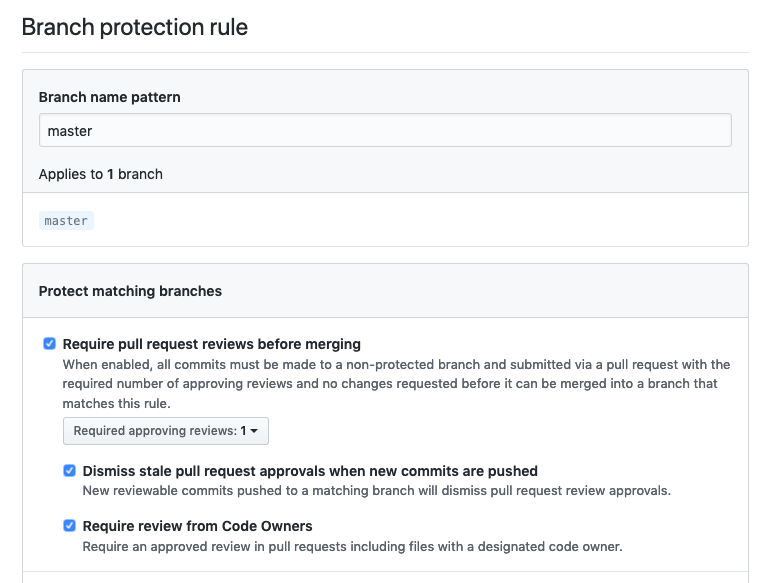
\includegraphics[scale=0.50]{images/github-branch-protection.png}
\caption{Setting up branch protection.}
\label{branchprotect}
\end{figure}

\justifying
After we start to work with CI/CD tools (status checks, like GitHub Actions for example) new choices, as seen in figure \ref{statuscheck}, become
available in this part of your repository for managing those checks.

\begin{figure}
\centering
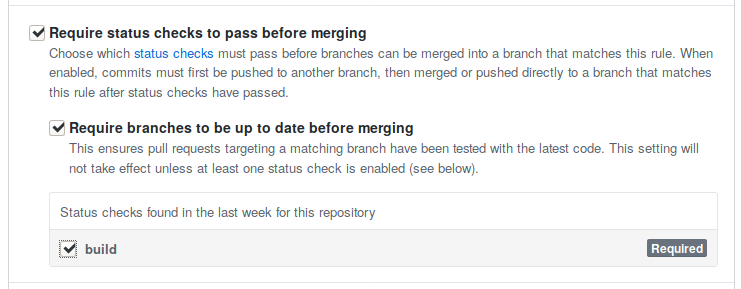
\includegraphics[scale=0.53]{images/guthub-status-check.png}
\caption{Requiring status checks.}
\label{statuscheck}
\end{figure}

\section{Branching and Merging}

When we say we are going to create a branch with git, it simply means we are going to take a snapshot of the code base at a point in time, and make our changes on that snapshot. The goal is to be able to make fixes and improvements without impacting the original code base.
Once our changes are completed, the typical process is to request a review from other team members and do some testing to make sure the changes will perform as expected. Once this is done, we are ready to merge our updated branch back into the main code base.

\subsection{Working with Branches}

\justifying
Naming your branches something useful is helpful (self documenting). Let's look at how to create a branch.

\subsection{Pull Requests}

\justifying
When you make changes on a local branch, say on your personal laptop, you will eventually want those changes
to flow back into the main project. Opening a pull request\index{Pull Request} is a means of letting other
people know you've got a set of changes ready for review and potential changes.

\justifying
Keeping pull requests smaller and more frequent makes it easier for your
peers to review your changes. It also means you will be less likely to lose work.

\subsection{Merging Your Branch}

\markdownInput{../labs/ch5/lab-5b.md}

\section{Forking and Cloning Existing Repositories}

\justifying
When someone else has a project on github.com that you would like to make changes to, you can make a ``fork'' of that project.
Forking\index{forking} a repository means you are making a copy of that repository to your personal account on the GitHub web
site. The reason for creating a fork is so we can make and test changes without any impact on the original repository.

\justifying
Once you have created a fork, you create a local copy of your fork on one or more of your personal workstations. This is
known as creating a ``clone'' \index{cloning a repo} of your fork. Now we have a workspace to make and test changes without
any impact to the parent repository. These changes or completed by creating one or more ``branches''. These branches and the
changes they encompass can be tested further, and are eventually merged into the parent repository.

\begin{figure}[!htb]
\centering

\begin{tikzpicture}[>=latex,line join=bevel,]
  \pgfsetlinewidth{1bp}
%%
\pgfsetcolor{black}
  % Edge: orig -> fork
  \draw [->] (178.26bp,143.83bp) .. controls (169.13bp,135.07bp) and (158.04bp,124.42bp)  .. (140.85bp,107.91bp);
  % Edge: fork -> clone
  \draw [->] (140.73bp,72.202bp) .. controls (150.06bp,63.242bp) and (161.52bp,52.241bp)  .. (179.12bp,35.345bp);
  % Edge: clone -> orig
  \draw [->] (222.15bp,34.664bp) .. controls (233.94bp,44.073bp) and (246.8bp,56.959bp)  .. (253.19bp,72.0bp) .. controls (259.45bp,86.726bp) and (259.45bp,93.274bp)  .. (253.19bp,108.0bp) .. controls (248.45bp,119.15bp) and (240.16bp,129.12bp)  .. (223.62bp,144.15bp);
  % Node: orig
\begin{scope}
  \definecolor{strokecol}{rgb}{0.0,0.0,0.0};
  \pgfsetstrokecolor{strokecol}
  \draw (197.19bp,162.0bp) ellipse (168.97bp and 18.0bp);
  \draw (197.19bp,162.0bp) node {Original Repository on github.com};
\end{scope}
  % Node: fork
\begin{scope}
  \definecolor{strokecol}{rgb}{0.0,0.0,0.0};
  \pgfsetstrokecolor{strokecol}
  \draw (122.19bp,90.0bp) ellipse (122.38bp and 18.0bp);
  \draw (122.19bp,90.0bp) node {Your fork on github.com};
\end{scope}
  % Node: clone
\begin{scope}
  \definecolor{strokecol}{rgb}{0.0,0.0,0.0};
  \pgfsetstrokecolor{strokecol}
  \draw (197.19bp,18.0bp) ellipse (64.19bp and 18.0bp);
  \draw (197.19bp,18.0bp) node {Local Clone};
\end{scope}
%
\end{tikzpicture}


\caption{Forking and cloning.}
\label{forkandclone}
\end{figure}

\justifying
This can be a tricky pattern to master, but it is fundamental if you
want to join the ranks of Open Source contributors and developers that
enjoy the full power of Git and GitHub.

\justifying
Adding a ``remote'' to your repository clone is a git convention to easily manage branches between your clone and
the original source repository.

\justifying
If you are starting out on a new project, simply creating a repo is probably enough. The whole fork/clone/merge to original
paradigm is better suited to medium to large size projects that accept contributions from multiple developers.

\markdownInput{../labs/ch5/lab-5c.md}

\section{Template Repositories}

\justifying
A GitHub Template Repository is available should you decide to follow along with the code examples in this book. The next sets of steps are
predicated on having Docker installed and running as described in the previous chapter.

\markdownInput{../labs/ch5/lab-5d.md}

\section{Conventions}

\subsection{CODEOWNERS}

\justifying
Creating a CODEOWNERS\index{CODEOWNERS} file is a good way to automatically tag folks in pull requests to make them aware of
changes to certain files or folders in your projects.

\justifying
In it's most basic form, the CODEOWNERS file in the .github directory simply lists the file(s) and the owner(s) on a line together.

\justifying
Consider this example where we add the ``@kevinflynn'' user to the CODEOWNERS file.

\begin{mybox}{\thetcbcounter: Adding a user to CODEOWNERS file}
      \lstinputlisting{code/22-github/create-codeowners.txt}
\end{mybox}

\justifying
In this example, the ``@kevinflynn'' user will be tagged as a reviewer in all pull requests.

\subsection{The .gitignore file}

\justifying
Use this file\index{.gitignore} to designate items that should be excluded from revision
control. This is useful for helping keep credentials and other secrets out of the GitHub repository.

\justifying
Consider the following example .gitignore file. This will prevent you from checking in the .DS-Store that
Macintosh creates in many folders.

\begin{mybox}{\thetcbcounter: Example .gitignore file}
      \lstinputlisting{code/22-github/create-gitignore.txt}
\end{mybox}

\section{Automated Repository Scanning}

\justifying
There are many GitHub plugins that are free for single-user/non-commercial scenarios. a cursory search of the web of the
GitHub Marketplace will turn up many of these. Let's leave some of the
tedious work to the bots, allowing us to focus on our DevSecOps journey to the cloud!

\justifying
\begin{tabular}{| p{2.3cm}| p{4.5cm} | p{8.5cm} |}
      \hline
     \textbf{Tool}& \textbf{Purpose}& \textbf{Source} \\
      \hline
      Renovate & dependency scanner & web site \\
      \hline
      lgtm & puppet-lint & Looks Good To Me \url{http://puppet-lint.com/} \\
      \hline
      metabob & AI based code review tool & website \\
      \hline
      bridgecrew & PR security scanner & web site \\
      \hline
\end{tabular}

\section{Directory Structure}

\justifying
Relevant files and folders mentioned in this chapter are organized as seen below.

\begin{figure}[!htb]
      \centering
      \chapter{Revision Control}
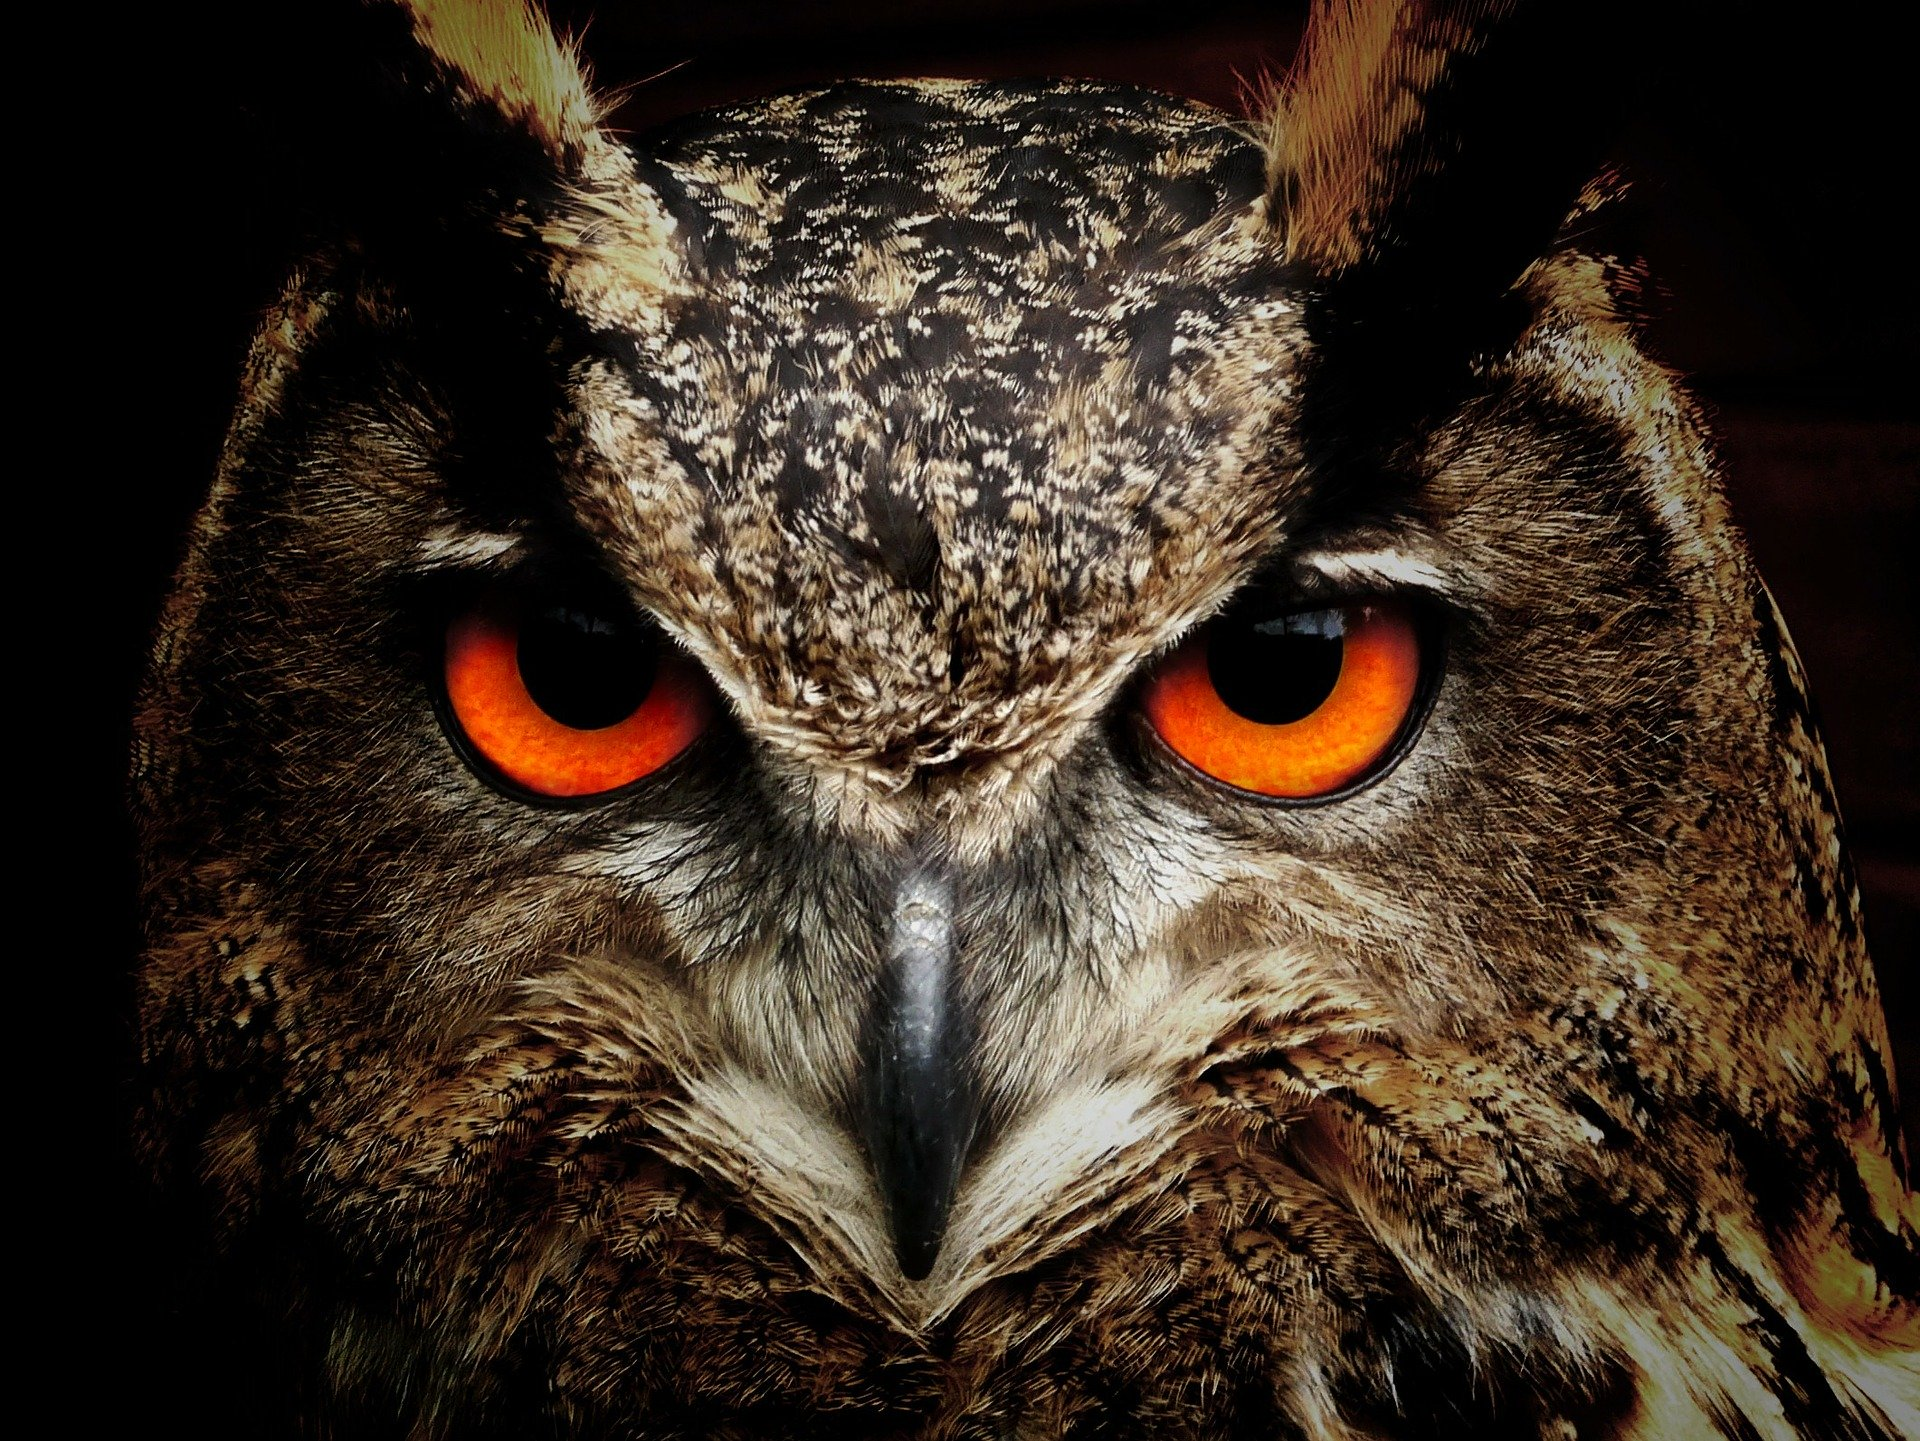
\includegraphics[scale=0.20]{images/owl-50267_1920.jpg}

\justifying
Using a revision control\index{revision control} methodology allows us to organize and store project artifacts. Typically these
artifacts are source code files but may include documentation, files to assist us with Kubernetes cluster management and application
deployment, and more. Websites like \href{https://github.com}{github.com} for example, are the modern
backbone of revision control, and foundational to our workflow. They are a key piece of our software delivery pipeline,
allowing us to declare a single source of truth for the code that makes up our project. Multiple users or teams can collaborate on a
single code base stored in a repository, the structure which encompasses a typical project. Even after the benefits from collaboration and
storage are considered, we can still realize a great benefit from being able to create releases, which can be tagged and ``rolled''
forward to and back from.

\justifying
There are other similar services we can choose from. These tend to be free for personal projects, non-commercial, and even some commercial
uses. For example \href{https://bitbucket.org/product}{Bitbucket} and \href{https://about.gitlab.com/}{GitLab}. For the purposes of this
book we will focus GitHub\index{GitHub}, since many people are familiar with it.

\justifying
Git is the tool that allows for revision control of your work. GitHub is a repository for storing that work, creating
teams to work on projects, tracking issues, defining release packages, and more. Simply put, \href{github.com}{github.com}
is a website that gives you a place to store the work you are using git to manage. Git was created in 2005 by
Linus Torvalds\index{Linus Torvalds}, who, as you may know, also created the Linux kernel.

\justifying
After creating your account on GitHub, one of the very first things you should do is to configure two-factor authentication (2FA)\index{2FA} for your GitHub account.
See \href{https://docs.github.com/en/github/authenticating-to-github/securing-your-account-with-two-factor-authentication-2fa}{securing your account with two factor authentication}
for more information. If you already have an account at GitHub, now is a good time to make sure you have this feature enabled. Two-factor authentication provides
an additional layer of security on your Github account, and is all-around good practice. Using two- or multi-factor authentication with a
password manager will do wonders
to improve your security hygiene. You may also use your password manager to store your account recovery codes. Creating a text file
that contains your recovery codes and keeping an encrypted copy in your home directory is another option.

\section{Creating a Repository}

Repository creation is well documented, for example
\href{https://docs.github.com/en/get-started/quickstart/create-a-repo}{these steps in the GitHub quick start pages}. Let look a bit
more closely ar what is involved in this process.

\justifying
Often I will start a new repository on my personal account while I use the steps in this book to get the project off the ground.
Later I will move the repository into an organization where the responsibility for ownership and administration can be
shared with other folks.

\justifying
Directions for the labs in this chapter are located in GitHub, of course!
\href{https://github.com/devsecfranklin/devsecops-tactical-workbook/tree/main/code/ch5}{Follow this link to view the lab files},
or simply proceed with the steps below.

\justifying
So far we have created the files seen in figure \ref{projfiles} to our project. There is much to be gained from bringing our project under revision control so let's
make that our next task. Take note, the ``top level'' for our GitHub repository will be the ``myproject'' folder even though we have some files in our ``/home/devsecops''
home directory that impact our project. We want to keep a separation between the source code and documentation in the ``myproject'' folder and any machine specific
configuration that is present on an individual developers workstation.

\begin{figure}[!htb]
\centering

\begin{tikzpicture}[>=latex,line join=bevel,]
  \pgfsetlinewidth{1bp}
%%
\pgfsetcolor{black}
  % Edge: framework -> pass
  \draw [->] (176.55bp,215.88bp) .. controls (156.36bp,206.39bp) and (131.08bp,194.51bp)  .. (100.33bp,180.07bp);
  % Edge: framework -> gnupg
  \draw [->] (203.36bp,215.7bp) .. controls (198.87bp,207.64bp) and (193.44bp,197.89bp)  .. (183.53bp,180.1bp);
  % Edge: framework -> docker
  \draw [->] (222.64bp,215.7bp) .. controls (227.13bp,207.64bp) and (232.56bp,197.89bp)  .. (242.47bp,180.1bp);
  % Edge: framework -> workspace
  \draw [->] (245.29bp,215.88bp) .. controls (262.87bp,206.55bp) and (284.81bp,194.92bp)  .. (312.59bp,180.19bp);
  % Edge: workspace -> myproject
  \draw [->] (345.0bp,143.7bp) .. controls (345.0bp,135.98bp) and (345.0bp,126.71bp)  .. (345.0bp,108.1bp);
  % Edge: myproject -> dockercom
  \draw [->] (328.19bp,71.697bp) .. controls (319.87bp,63.135bp) and (309.69bp,52.656bp)  .. (293.62bp,36.104bp);
  % Edge: myproject -> Dockerfile
  \draw [->] (361.81bp,71.697bp) .. controls (370.13bp,63.135bp) and (380.31bp,52.656bp)  .. (396.38bp,36.104bp);
  % Node: framework
\begin{scope}
  \definecolor{strokecol}{rgb}{0.0,0.0,0.0};
  \pgfsetstrokecolor{strokecol}
  \draw (274.0bp,252.0bp) -- (271.0bp,256.0bp) -- (250.0bp,256.0bp) -- (247.0bp,252.0bp) -- (152.0bp,252.0bp) -- (152.0bp,216.0bp) -- (274.0bp,216.0bp) -- cycle;
  \draw (213.0bp,234.0bp) node {/home/devsecops};
\end{scope}
  % Node: pass
\begin{scope}
  \definecolor{strokecol}{rgb}{0.0,0.0,0.0};
  \pgfsetstrokecolor{strokecol}
  \draw (128.0bp,180.0bp) -- (125.0bp,184.0bp) -- (104.0bp,184.0bp) -- (101.0bp,180.0bp) -- (0.0bp,180.0bp) -- (0.0bp,144.0bp) -- (128.0bp,144.0bp) -- cycle;
  \draw (64.0bp,162.0bp) node {.password-store};
\end{scope}
  % Node: gnupg
\begin{scope}
  \definecolor{strokecol}{rgb}{0.0,0.0,0.0};
  \pgfsetstrokecolor{strokecol}
  \draw (202.0bp,180.0bp) -- (199.0bp,184.0bp) -- (178.0bp,184.0bp) -- (175.0bp,180.0bp) -- (146.0bp,180.0bp) -- (146.0bp,144.0bp) -- (202.0bp,144.0bp) -- cycle;
  \draw (174.0bp,162.0bp) node {.gnupg};
\end{scope}
  % Node: docker
\begin{scope}
  \definecolor{strokecol}{rgb}{0.0,0.0,0.0};
  \pgfsetstrokecolor{strokecol}
  \draw (283.5bp,180.0bp) -- (280.5bp,184.0bp) -- (259.5bp,184.0bp) -- (256.5bp,180.0bp) -- (220.5bp,180.0bp) -- (220.5bp,144.0bp) -- (283.5bp,144.0bp) -- cycle;
  \draw (252.0bp,162.0bp) node {.docker};
\end{scope}
  % Node: workspace
\begin{scope}
  \definecolor{strokecol}{rgb}{0.0,0.0,0.0};
  \pgfsetstrokecolor{strokecol}
  \draw (388.5bp,180.0bp) -- (385.5bp,184.0bp) -- (364.5bp,184.0bp) -- (361.5bp,180.0bp) -- (301.5bp,180.0bp) -- (301.5bp,144.0bp) -- (388.5bp,144.0bp) -- cycle;
  \draw (345.0bp,162.0bp) node {workspace};
\end{scope}
  % Node: myproject
\begin{scope}
  \definecolor{strokecol}{rgb}{0.0,0.0,0.0};
  \pgfsetstrokecolor{strokecol}
  \draw (387.5bp,108.0bp) -- (384.5bp,112.0bp) -- (363.5bp,112.0bp) -- (360.5bp,108.0bp) -- (302.5bp,108.0bp) -- (302.5bp,72.0bp) -- (387.5bp,72.0bp) -- cycle;
  \draw (345.0bp,90.0bp) node {myproject};
\end{scope}
  % Node: dockercom
\begin{scope}
  \definecolor{strokecol}{rgb}{0.0,0.0,0.0};
  \pgfsetstrokecolor{strokecol}
  \draw (351.5bp,36.0bp) -- (202.5bp,36.0bp) -- (202.5bp,0.0bp) -- (351.5bp,0.0bp) -- cycle;
  \draw (277.0bp,18.0bp) node {docker-compose.yml};
\end{scope}
  % Node: Dockerfile
\begin{scope}
  \definecolor{strokecol}{rgb}{0.0,0.0,0.0};
  \pgfsetstrokecolor{strokecol}
  \draw (456.0bp,36.0bp) -- (370.0bp,36.0bp) -- (370.0bp,0.0bp) -- (456.0bp,0.0bp) -- cycle;
  \draw (413.0bp,18.0bp) node {Dockerfile};
\end{scope}
%
\end{tikzpicture}


\caption{Project files.}
\label{projfiles}
\end{figure}

\markdownInput{../labs/ch5/lab-5a.md}

\subsection{Repository Settings}

\justifying
When setting up a new repository in my GitHub account, I always click the Settings tab (with the little gear icon) and then choose the
``Branches'' section. The Default branch gets set to ``main''. Clicking the ``Add Rule'' button, entering ``main'' for the ``Branch name pattern'',
and then the green ``Create'' button sets up master as a protected branch. Consider the following example \ref{branchprotect}.

\begin{figure}[!htb]
\centering
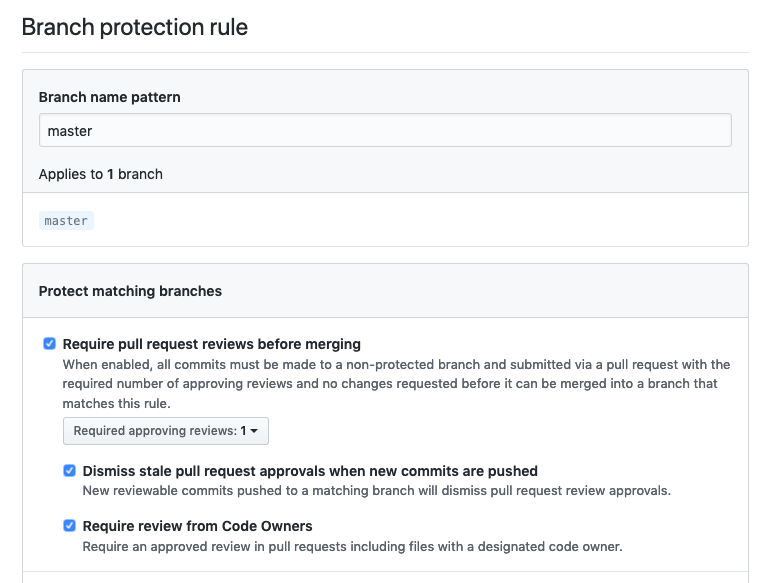
\includegraphics[scale=0.50]{images/github-branch-protection.png}
\caption{Setting up branch protection.}
\label{branchprotect}
\end{figure}

\justifying
After we start to work with CI/CD tools (status checks, like GitHub Actions for example) new choices, as seen in figure \ref{statuscheck}, become
available in this part of your repository for managing those checks.

\begin{figure}
\centering
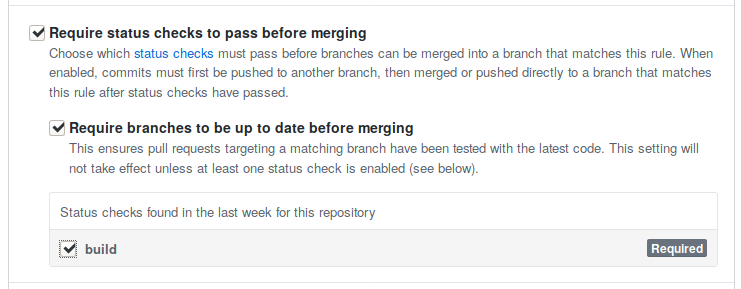
\includegraphics[scale=0.53]{images/guthub-status-check.png}
\caption{Requiring status checks.}
\label{statuscheck}
\end{figure}

\section{Branching and Merging}

When we say we are going to create a branch with git, it simply means we are going to take a snapshot of the code base at a point in time, and make our changes on that snapshot. The goal is to be able to make fixes and improvements without impacting the original code base.
Once our changes are completed, the typical process is to request a review from other team members and do some testing to make sure the changes will perform as expected. Once this is done, we are ready to merge our updated branch back into the main code base.

\subsection{Working with Branches}

\justifying
Naming your branches something useful is helpful (self documenting). Let's look at how to create a branch.

\subsection{Pull Requests}

\justifying
When you make changes on a local branch, say on your personal laptop, you will eventually want those changes
to flow back into the main project. Opening a pull request\index{Pull Request} is a means of letting other
people know you've got a set of changes ready for review and potential changes.

\justifying
Keeping pull requests smaller and more frequent makes it easier for your
peers to review your changes. It also means you will be less likely to lose work.

\subsection{Merging Your Branch}

\markdownInput{../labs/ch5/lab-5b.md}

\section{Forking and Cloning Existing Repositories}

\justifying
When someone else has a project on github.com that you would like to make changes to, you can make a ``fork'' of that project.
Forking\index{forking} a repository means you are making a copy of that repository to your personal account on the GitHub web
site. The reason for creating a fork is so we can make and test changes without any impact on the original repository.

\justifying
Once you have created a fork, you create a local copy of your fork on one or more of your personal workstations. This is
known as creating a ``clone'' \index{cloning a repo} of your fork. Now we have a workspace to make and test changes without
any impact to the parent repository. These changes or completed by creating one or more ``branches''. These branches and the
changes they encompass can be tested further, and are eventually merged into the parent repository.

\begin{figure}[!htb]
\centering

\begin{tikzpicture}[>=latex,line join=bevel,]
  \pgfsetlinewidth{1bp}
%%
\pgfsetcolor{black}
  % Edge: orig -> fork
  \draw [->] (178.26bp,143.83bp) .. controls (169.13bp,135.07bp) and (158.04bp,124.42bp)  .. (140.85bp,107.91bp);
  % Edge: fork -> clone
  \draw [->] (140.73bp,72.202bp) .. controls (150.06bp,63.242bp) and (161.52bp,52.241bp)  .. (179.12bp,35.345bp);
  % Edge: clone -> orig
  \draw [->] (222.15bp,34.664bp) .. controls (233.94bp,44.073bp) and (246.8bp,56.959bp)  .. (253.19bp,72.0bp) .. controls (259.45bp,86.726bp) and (259.45bp,93.274bp)  .. (253.19bp,108.0bp) .. controls (248.45bp,119.15bp) and (240.16bp,129.12bp)  .. (223.62bp,144.15bp);
  % Node: orig
\begin{scope}
  \definecolor{strokecol}{rgb}{0.0,0.0,0.0};
  \pgfsetstrokecolor{strokecol}
  \draw (197.19bp,162.0bp) ellipse (168.97bp and 18.0bp);
  \draw (197.19bp,162.0bp) node {Original Repository on github.com};
\end{scope}
  % Node: fork
\begin{scope}
  \definecolor{strokecol}{rgb}{0.0,0.0,0.0};
  \pgfsetstrokecolor{strokecol}
  \draw (122.19bp,90.0bp) ellipse (122.38bp and 18.0bp);
  \draw (122.19bp,90.0bp) node {Your fork on github.com};
\end{scope}
  % Node: clone
\begin{scope}
  \definecolor{strokecol}{rgb}{0.0,0.0,0.0};
  \pgfsetstrokecolor{strokecol}
  \draw (197.19bp,18.0bp) ellipse (64.19bp and 18.0bp);
  \draw (197.19bp,18.0bp) node {Local Clone};
\end{scope}
%
\end{tikzpicture}


\caption{Forking and cloning.}
\label{forkandclone}
\end{figure}

\justifying
This can be a tricky pattern to master, but it is fundamental if you
want to join the ranks of Open Source contributors and developers that
enjoy the full power of Git and GitHub.

\justifying
Adding a ``remote'' to your repository clone is a git convention to easily manage branches between your clone and
the original source repository.

\justifying
If you are starting out on a new project, simply creating a repo is probably enough. The whole fork/clone/merge to original
paradigm is better suited to medium to large size projects that accept contributions from multiple developers.

\markdownInput{../labs/ch5/lab-5c.md}

\section{Template Repositories}

\justifying
A GitHub Template Repository is available should you decide to follow along with the code examples in this book. The next sets of steps are
predicated on having Docker installed and running as described in the previous chapter.

\markdownInput{../labs/ch5/lab-5d.md}

\section{Conventions}

\subsection{CODEOWNERS}

\justifying
Creating a CODEOWNERS\index{CODEOWNERS} file is a good way to automatically tag folks in pull requests to make them aware of
changes to certain files or folders in your projects.

\justifying
In it's most basic form, the CODEOWNERS file in the .github directory simply lists the file(s) and the owner(s) on a line together.

\justifying
Consider this example where we add the ``@kevinflynn'' user to the CODEOWNERS file.

\begin{mybox}{\thetcbcounter: Adding a user to CODEOWNERS file}
      \lstinputlisting{code/22-github/create-codeowners.txt}
\end{mybox}

\justifying
In this example, the ``@kevinflynn'' user will be tagged as a reviewer in all pull requests.

\subsection{The .gitignore file}

\justifying
Use this file\index{.gitignore} to designate items that should be excluded from revision
control. This is useful for helping keep credentials and other secrets out of the GitHub repository.

\justifying
Consider the following example .gitignore file. This will prevent you from checking in the .DS-Store that
Macintosh creates in many folders.

\begin{mybox}{\thetcbcounter: Example .gitignore file}
      \lstinputlisting{code/22-github/create-gitignore.txt}
\end{mybox}

\section{Automated Repository Scanning}

\justifying
There are many GitHub plugins that are free for single-user/non-commercial scenarios. a cursory search of the web of the
GitHub Marketplace will turn up many of these. Let's leave some of the
tedious work to the bots, allowing us to focus on our DevSecOps journey to the cloud!

\justifying
\begin{tabular}{| p{2.3cm}| p{4.5cm} | p{8.5cm} |}
      \hline
     \textbf{Tool}& \textbf{Purpose}& \textbf{Source} \\
      \hline
      Renovate & dependency scanner & web site \\
      \hline
      lgtm & puppet-lint & Looks Good To Me \url{http://puppet-lint.com/} \\
      \hline
      metabob & AI based code review tool & website \\
      \hline
      bridgecrew & PR security scanner & web site \\
      \hline
\end{tabular}

\section{Directory Structure}

\justifying
Relevant files and folders mentioned in this chapter are organized as seen below.

\begin{figure}[!htb]
      \centering
      \chapter{Revision Control}
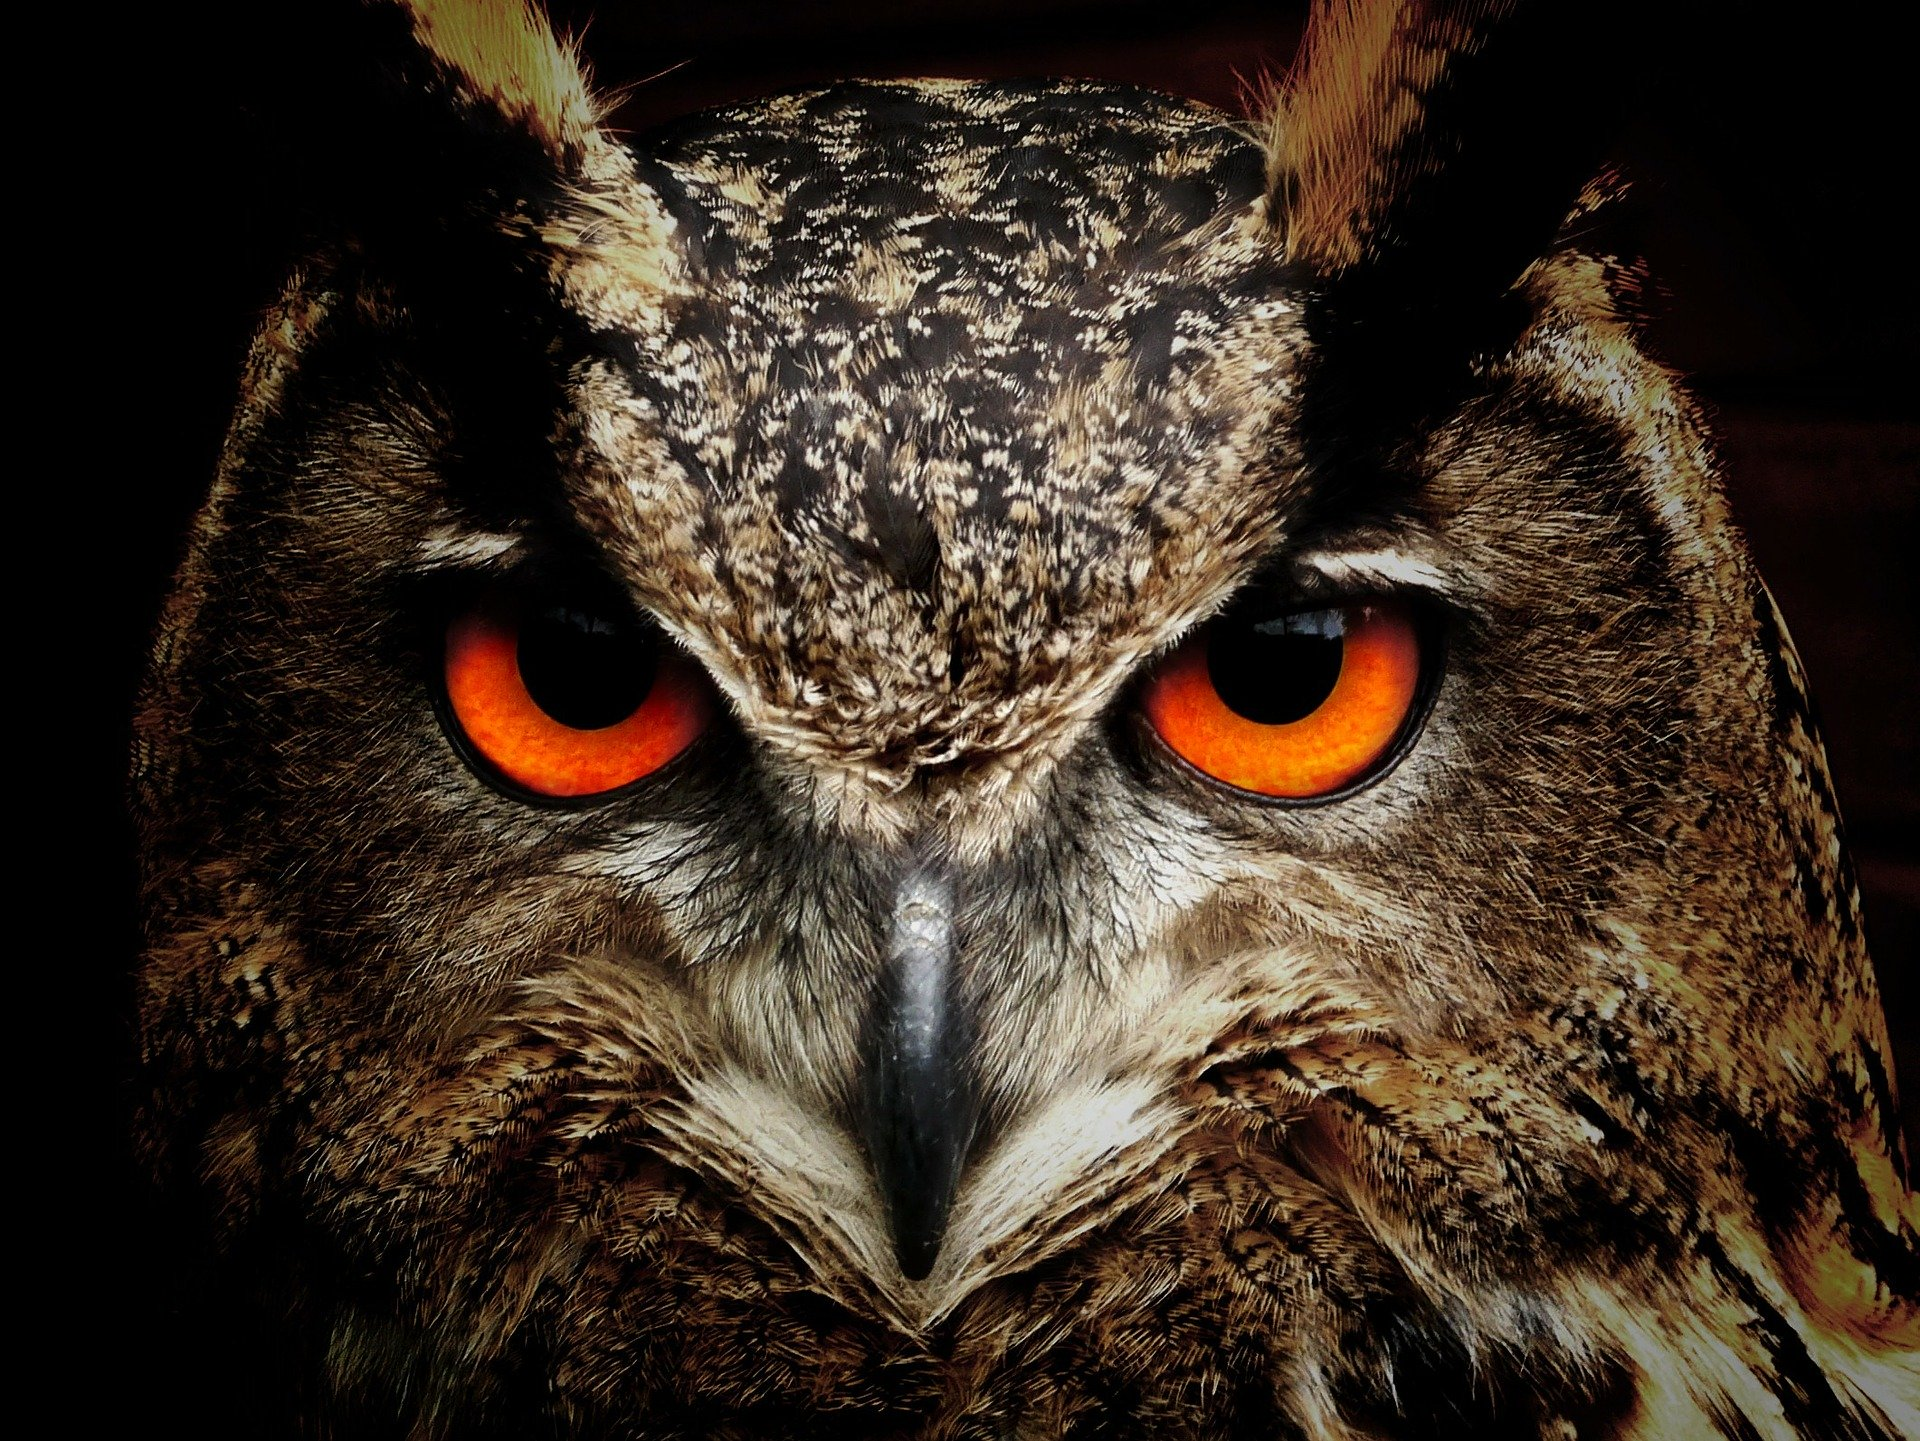
\includegraphics[scale=0.20]{images/owl-50267_1920.jpg}

\justifying
Using a revision control\index{revision control} methodology allows us to organize and store project artifacts. Typically these
artifacts are source code files but may include documentation, files to assist us with Kubernetes cluster management and application
deployment, and more. Websites like \href{https://github.com}{github.com} for example, are the modern
backbone of revision control, and foundational to our workflow. They are a key piece of our software delivery pipeline,
allowing us to declare a single source of truth for the code that makes up our project. Multiple users or teams can collaborate on a
single code base stored in a repository, the structure which encompasses a typical project. Even after the benefits from collaboration and
storage are considered, we can still realize a great benefit from being able to create releases, which can be tagged and ``rolled''
forward to and back from.

\justifying
There are other similar services we can choose from. These tend to be free for personal projects, non-commercial, and even some commercial
uses. For example \href{https://bitbucket.org/product}{Bitbucket} and \href{https://about.gitlab.com/}{GitLab}. For the purposes of this
book we will focus GitHub\index{GitHub}, since many people are familiar with it.

\justifying
Git is the tool that allows for revision control of your work. GitHub is a repository for storing that work, creating
teams to work on projects, tracking issues, defining release packages, and more. Simply put, \href{github.com}{github.com}
is a website that gives you a place to store the work you are using git to manage. Git was created in 2005 by
Linus Torvalds\index{Linus Torvalds}, who, as you may know, also created the Linux kernel.

\justifying
After creating your account on GitHub, one of the very first things you should do is to configure two-factor authentication (2FA)\index{2FA} for your GitHub account.
See \href{https://docs.github.com/en/github/authenticating-to-github/securing-your-account-with-two-factor-authentication-2fa}{securing your account with two factor authentication}
for more information. If you already have an account at GitHub, now is a good time to make sure you have this feature enabled. Two-factor authentication provides
an additional layer of security on your Github account, and is all-around good practice. Using two- or multi-factor authentication with a
password manager will do wonders
to improve your security hygiene. You may also use your password manager to store your account recovery codes. Creating a text file
that contains your recovery codes and keeping an encrypted copy in your home directory is another option.

\section{Creating a Repository}

Repository creation is well documented, for example
\href{https://docs.github.com/en/get-started/quickstart/create-a-repo}{these steps in the GitHub quick start pages}. Let look a bit
more closely ar what is involved in this process.

\justifying
Often I will start a new repository on my personal account while I use the steps in this book to get the project off the ground.
Later I will move the repository into an organization where the responsibility for ownership and administration can be
shared with other folks.

\justifying
Directions for the labs in this chapter are located in GitHub, of course!
\href{https://github.com/devsecfranklin/devsecops-tactical-workbook/tree/main/code/ch5}{Follow this link to view the lab files},
or simply proceed with the steps below.

\justifying
So far we have created the files seen in figure \ref{projfiles} to our project. There is much to be gained from bringing our project under revision control so let's
make that our next task. Take note, the ``top level'' for our GitHub repository will be the ``myproject'' folder even though we have some files in our ``/home/devsecops''
home directory that impact our project. We want to keep a separation between the source code and documentation in the ``myproject'' folder and any machine specific
configuration that is present on an individual developers workstation.

\begin{figure}[!htb]
\centering
\input{dot/22-gh-prelab.tex}
\caption{Project files.}
\label{projfiles}
\end{figure}

\markdownInput{../labs/ch5/lab-5a.md}

\subsection{Repository Settings}

\justifying
When setting up a new repository in my GitHub account, I always click the Settings tab (with the little gear icon) and then choose the
``Branches'' section. The Default branch gets set to ``main''. Clicking the ``Add Rule'' button, entering ``main'' for the ``Branch name pattern'',
and then the green ``Create'' button sets up master as a protected branch. Consider the following example \ref{branchprotect}.

\begin{figure}[!htb]
\centering
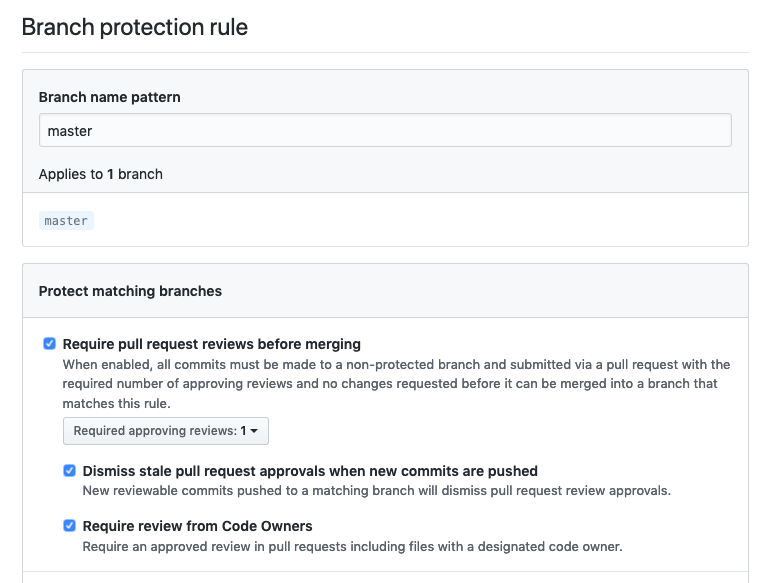
\includegraphics[scale=0.50]{images/github-branch-protection.png}
\caption{Setting up branch protection.}
\label{branchprotect}
\end{figure}

\justifying
After we start to work with CI/CD tools (status checks, like GitHub Actions for example) new choices, as seen in figure \ref{statuscheck}, become
available in this part of your repository for managing those checks.

\begin{figure}
\centering
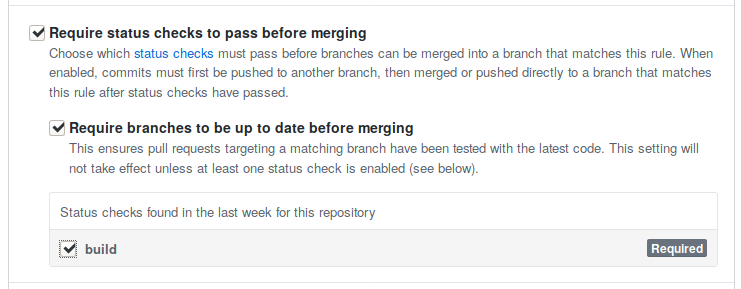
\includegraphics[scale=0.53]{images/guthub-status-check.png}
\caption{Requiring status checks.}
\label{statuscheck}
\end{figure}

\section{Branching and Merging}

When we say we are going to create a branch with git, it simply means we are going to take a snapshot of the code base at a point in time, and make our changes on that snapshot. The goal is to be able to make fixes and improvements without impacting the original code base.
Once our changes are completed, the typical process is to request a review from other team members and do some testing to make sure the changes will perform as expected. Once this is done, we are ready to merge our updated branch back into the main code base.

\subsection{Working with Branches}

\justifying
Naming your branches something useful is helpful (self documenting). Let's look at how to create a branch.

\subsection{Pull Requests}

\justifying
When you make changes on a local branch, say on your personal laptop, you will eventually want those changes
to flow back into the main project. Opening a pull request\index{Pull Request} is a means of letting other
people know you've got a set of changes ready for review and potential changes.

\justifying
Keeping pull requests smaller and more frequent makes it easier for your
peers to review your changes. It also means you will be less likely to lose work.

\subsection{Merging Your Branch}

\markdownInput{../labs/ch5/lab-5b.md}

\section{Forking and Cloning Existing Repositories}

\justifying
When someone else has a project on github.com that you would like to make changes to, you can make a ``fork'' of that project.
Forking\index{forking} a repository means you are making a copy of that repository to your personal account on the GitHub web
site. The reason for creating a fork is so we can make and test changes without any impact on the original repository.

\justifying
Once you have created a fork, you create a local copy of your fork on one or more of your personal workstations. This is
known as creating a ``clone'' \index{cloning a repo} of your fork. Now we have a workspace to make and test changes without
any impact to the parent repository. These changes or completed by creating one or more ``branches''. These branches and the
changes they encompass can be tested further, and are eventually merged into the parent repository.

\begin{figure}[!htb]
\centering
\input{dot/forking.tex}
\caption{Forking and cloning.}
\label{forkandclone}
\end{figure}

\justifying
This can be a tricky pattern to master, but it is fundamental if you
want to join the ranks of Open Source contributors and developers that
enjoy the full power of Git and GitHub.

\justifying
Adding a ``remote'' to your repository clone is a git convention to easily manage branches between your clone and
the original source repository.

\justifying
If you are starting out on a new project, simply creating a repo is probably enough. The whole fork/clone/merge to original
paradigm is better suited to medium to large size projects that accept contributions from multiple developers.

\markdownInput{../labs/ch5/lab-5c.md}

\section{Template Repositories}

\justifying
A GitHub Template Repository is available should you decide to follow along with the code examples in this book. The next sets of steps are
predicated on having Docker installed and running as described in the previous chapter.

\markdownInput{../labs/ch5/lab-5d.md}

\section{Conventions}

\subsection{CODEOWNERS}

\justifying
Creating a CODEOWNERS\index{CODEOWNERS} file is a good way to automatically tag folks in pull requests to make them aware of
changes to certain files or folders in your projects.

\justifying
In it's most basic form, the CODEOWNERS file in the .github directory simply lists the file(s) and the owner(s) on a line together.

\justifying
Consider this example where we add the ``@kevinflynn'' user to the CODEOWNERS file.

\begin{mybox}{\thetcbcounter: Adding a user to CODEOWNERS file}
      \lstinputlisting{code/22-github/create-codeowners.txt}
\end{mybox}

\justifying
In this example, the ``@kevinflynn'' user will be tagged as a reviewer in all pull requests.

\subsection{The .gitignore file}

\justifying
Use this file\index{.gitignore} to designate items that should be excluded from revision
control. This is useful for helping keep credentials and other secrets out of the GitHub repository.

\justifying
Consider the following example .gitignore file. This will prevent you from checking in the .DS-Store that
Macintosh creates in many folders.

\begin{mybox}{\thetcbcounter: Example .gitignore file}
      \lstinputlisting{code/22-github/create-gitignore.txt}
\end{mybox}

\section{Automated Repository Scanning}

\justifying
There are many GitHub plugins that are free for single-user/non-commercial scenarios. a cursory search of the web of the
GitHub Marketplace will turn up many of these. Let's leave some of the
tedious work to the bots, allowing us to focus on our DevSecOps journey to the cloud!

\justifying
\begin{tabular}{| p{2.3cm}| p{4.5cm} | p{8.5cm} |}
      \hline
     \textbf{Tool}& \textbf{Purpose}& \textbf{Source} \\
      \hline
      Renovate & dependency scanner & web site \\
      \hline
      lgtm & puppet-lint & Looks Good To Me \url{http://puppet-lint.com/} \\
      \hline
      metabob & AI based code review tool & website \\
      \hline
      bridgecrew & PR security scanner & web site \\
      \hline
\end{tabular}

\section{Directory Structure}

\justifying
Relevant files and folders mentioned in this chapter are organized as seen below.

\begin{figure}[!htb]
      \centering
      \input{dot/22-github.tex}
      \caption{GitHub related files.}
      \label{githubfiles}
\end{figure}

      \caption{GitHub related files.}
      \label{githubfiles}
\end{figure}

      \caption{GitHub related files.}
      \label{githubfiles}
\end{figure}

\chapter{GNU Makefiles}


\includegraphics[scale=0.20]{images/books-1163695_1920.jpg}

\begin{displayquote}
	\emph{Make originated with a visit from Steve Johnson (author of yacc, etc.), storming into my office, cursing the Fates that had caused him to waste a morning debugging a correct program (bug had been fixed, file hadn't been compiled, cc *.o was therefore unaffected). As I had spent a part of the previous evening coping with the same disaster on a project I was working on, the idea of a tool to solve it came up. It began with an elaborate idea of a dependency analyzer, boiled down to something much simpler, and turned into Make that weekend. Use of tools that were still wet was part of the culture. Makefiles were text files, not magically encoded binaries, because that was the Unix ethos: printable, debuggable, understandable stuff.}
	
	Stuart Feldman\cite{raymond2004programming}
\end{displayquote}


\justify{}
The GNU make tool is still around decades later for a reason. It has been battle-tested over the years and become a key tool for folks like us. Originally intended for use in UNIX systems as an aid when compiling C projects, make is a handy way to put short sets of frequently used shell commands at our fingertips. For make to function properly, you must create a Makefile\index{Makefile} in the directory
you invoke the make command from. Using a Makefile lets us avoid typing complicated and hard to recall strings on the command
line. You can simply type ``make docker'' and have everything build as desired from a list of commands in part of your Makefile. This is beneficial when
you have lots of arguments and environment variables that you and your team members need for sets of commands
to work properly. When your team member invokes a specific rule from a Makefile, it works without you having to 
help them configure things or make them aware of all the parameters. We're going to be using \href{https://www.gnu.org/software/make/}{GNU Make} for our projects.

\justify{}
With Python projects, I like to use make to kick off builds and unit tests in a virtual environment, perhaps with differing sets of requirements files. When we build a python application we might call on ``requirements.txt'' for the dependencies we need. When we test, we might have another file called ``requirements-test.txt'' that gets installed with or in place of the usual requirements. Similarly with Ruby, there may be a need for different Gemfiles depending on your activity. Using make with Docker and docker-compose can be beneficial for building and running images locally. 

\justify{}
A Makefile can be as simple as a few lines or grow to become an extremely intricate and vital piece of your
build environment. You might like to have a look at 
\href{https://www.gnu.org/software/make/manual/make.html#Introduction}{the GNU make manual} at least once just to get a feel for how they work.

\justify{}
When a Makefile is executed, you can use the ampersand character to suppress the printing of lines from the original Makefile.

\section{Rules}

\justify{}
Makefiles are comprised of various stanzas, know as rules. This is where the work gets done. Let's add a rule
for Docker and a target for Python to make our lives easier in the future. Let's examine a simple Makefile with a single rules.

\justify{}
\begin{mybox}{\thetcbcounter: Our First Makefile}
	\lstinputlisting{code/23-makefiles/simple-makefile}
\end{mybox}

\justify{}
It's important to note that indentation of Makefiles is done using tabs rather than spaces. If your Makefile is failing, check for spots where lines were improperly
indented with eight spaces rather than a tab cahracter. The proper way to indent in a Makefile is to use tab characters.

\section{The PHONY Directive}

\justify{}
If a file or directory exists with the same name as a rule in the Makefile, you will need to specify
it under the PHONY directive. This will allow the Makefile to find and run the desired commands.

\justify{}
\begin{mybox}{\thetcbcounter: The PHONY Directive}
	\lstinputlisting{code/23-makefiles/phony-makefile}
\end{mybox}

\subsection{Understanding the PHONY Directive (Lab 6a)}

\subsubsection{Create a Small Makefile}
\justify{}
Create a small two-line Makefile. Be sure to use a tab character to indent the second line.

\begin{mybox}{\thetcbcounter: Small two-line Makefile}
	\lstinputlisting{code/23-makefiles/6a-create}
\end{mybox}

\subsubsection{Test the Makefile}

\justify{}
Test the Makefile by running the ``make'' command. Notice that you can
type ``make'' or ``make code'' and get the same result.

\begin{mybox}{\thetcbcounter: First Test}
	\lstinputlisting{code/23-makefiles/6a-test1}
\end{mybox}

\subsubsection{Test Again with PHONY}

\justify{}
Now edit the Makefile to include the PHONY directive. Be mindful of the 
leading dot character.

\begin{mybox}{\thetcbcounter: Add PHONY}
	\lstinputlisting{code/23-makefiles/6a-test2}
\end{mybox}

\justify{}
Try running make again.

\begin{mybox}{\thetcbcounter: Run make}
	\lstinputlisting{code/23-makefiles/6a-test3}
\end{mybox}

\justify{}
Note that the output occurs twice. To suppress the extra output, you can prepend the command with an ampersand character like so:

\begin{mybox}{\thetcbcounter: Supress extra Output}
	\lstinputlisting{code/23-makefiles/6a-test4}
\end{mybox}

\justify{}
Now try running one final time.

\begin{mybox}{\thetcbcounter: Supress extra Output}
	\lstinputlisting{code/23-makefiles/6a-test5}
\end{mybox}

\justify{}
Now we get the desired result without the printing of the command
by make.

\section{Variables and Conditionals in a Makefile}

\justify{}
Conditional operators and variables can be specified in a Makefile. Note that variables and conditionals do not observe the save rules with respect to tab based indentation.

\justify{}
Let's look at a simple Makefile example for checking if two programs are installed. Here we have a Makefile
with a single target, ``clean''. The first two lines of this Makefile run shell commands to determine 
whether ``kubectl'' and ``tkn'' are installed in the current environment. 

\begin{mybox}{\thetcbcounter: Conditionals and Variable Example}
	\lstinputlisting{{listing options={style=tcblatex,numbers=left,numberstyle=\tiny\color{red!75!black}}}code/23-makefiles/6b-Makefile}
\end{mybox}

\section{Large Example Makefile}
\justify{}
Let's consider a larger Makefile so we can get familiar with more of the elements.



\section{Further Reading}

\section{Directory Structure with Makefile}
\justify{}
Relevant files and folders related to our Makefile are organized as seen
below.

\begin{figure}[!htb]
	
\begin{tikzpicture}[>=latex,line join=bevel,]
  \pgfsetlinewidth{1bp}
%%
\pgfsetcolor{black}
  % Edge: devsecops -> Makefile
  \draw [->] (121.64bp,71.697bp) .. controls (115.77bp,63.474bp) and (108.63bp,53.483bp)  .. (96.217bp,36.104bp);
  % Edge: devsecops -> Dockerfile
  \draw [->] (146.36bp,71.697bp) .. controls (152.23bp,63.474bp) and (159.37bp,53.483bp)  .. (171.78bp,36.104bp);
  % Node: devsecops
\begin{scope}
  \definecolor{strokecol}{rgb}{0.0,0.0,0.0};
  \pgfsetstrokecolor{strokecol}
  \draw (268.0bp,108.0bp) -- (265.0bp,112.0bp) -- (244.0bp,112.0bp) -- (241.0bp,108.0bp) -- (0.0bp,108.0bp) -- (0.0bp,72.0bp) -- (268.0bp,72.0bp) -- cycle;
  \draw (134.0bp,90.0bp) node {/home/devsecops/workspace/myproject};
\end{scope}
  % Node: Makefile
\begin{scope}
  \definecolor{strokecol}{rgb}{0.0,0.0,0.0};
  \pgfsetstrokecolor{strokecol}
  \draw (122.5bp,36.0bp) -- (45.5bp,36.0bp) -- (45.5bp,0.0bp) -- (122.5bp,0.0bp) -- cycle;
  \draw (84.0bp,18.0bp) node {Makefile};
\end{scope}
  % Node: Dockerfile
\begin{scope}
  \definecolor{strokecol}{rgb}{0.0,0.0,0.0};
  \pgfsetstrokecolor{strokecol}
  \draw (227.0bp,36.0bp) -- (141.0bp,36.0bp) -- (141.0bp,0.0bp) -- (227.0bp,0.0bp) -- cycle;
  \draw (184.0bp,18.0bp) node {Dockerfile};
\end{scope}
%
\end{tikzpicture}


	\caption{Makefile and related files.}
\label{makefile}
\end{figure}


\chapter{Useful Python}

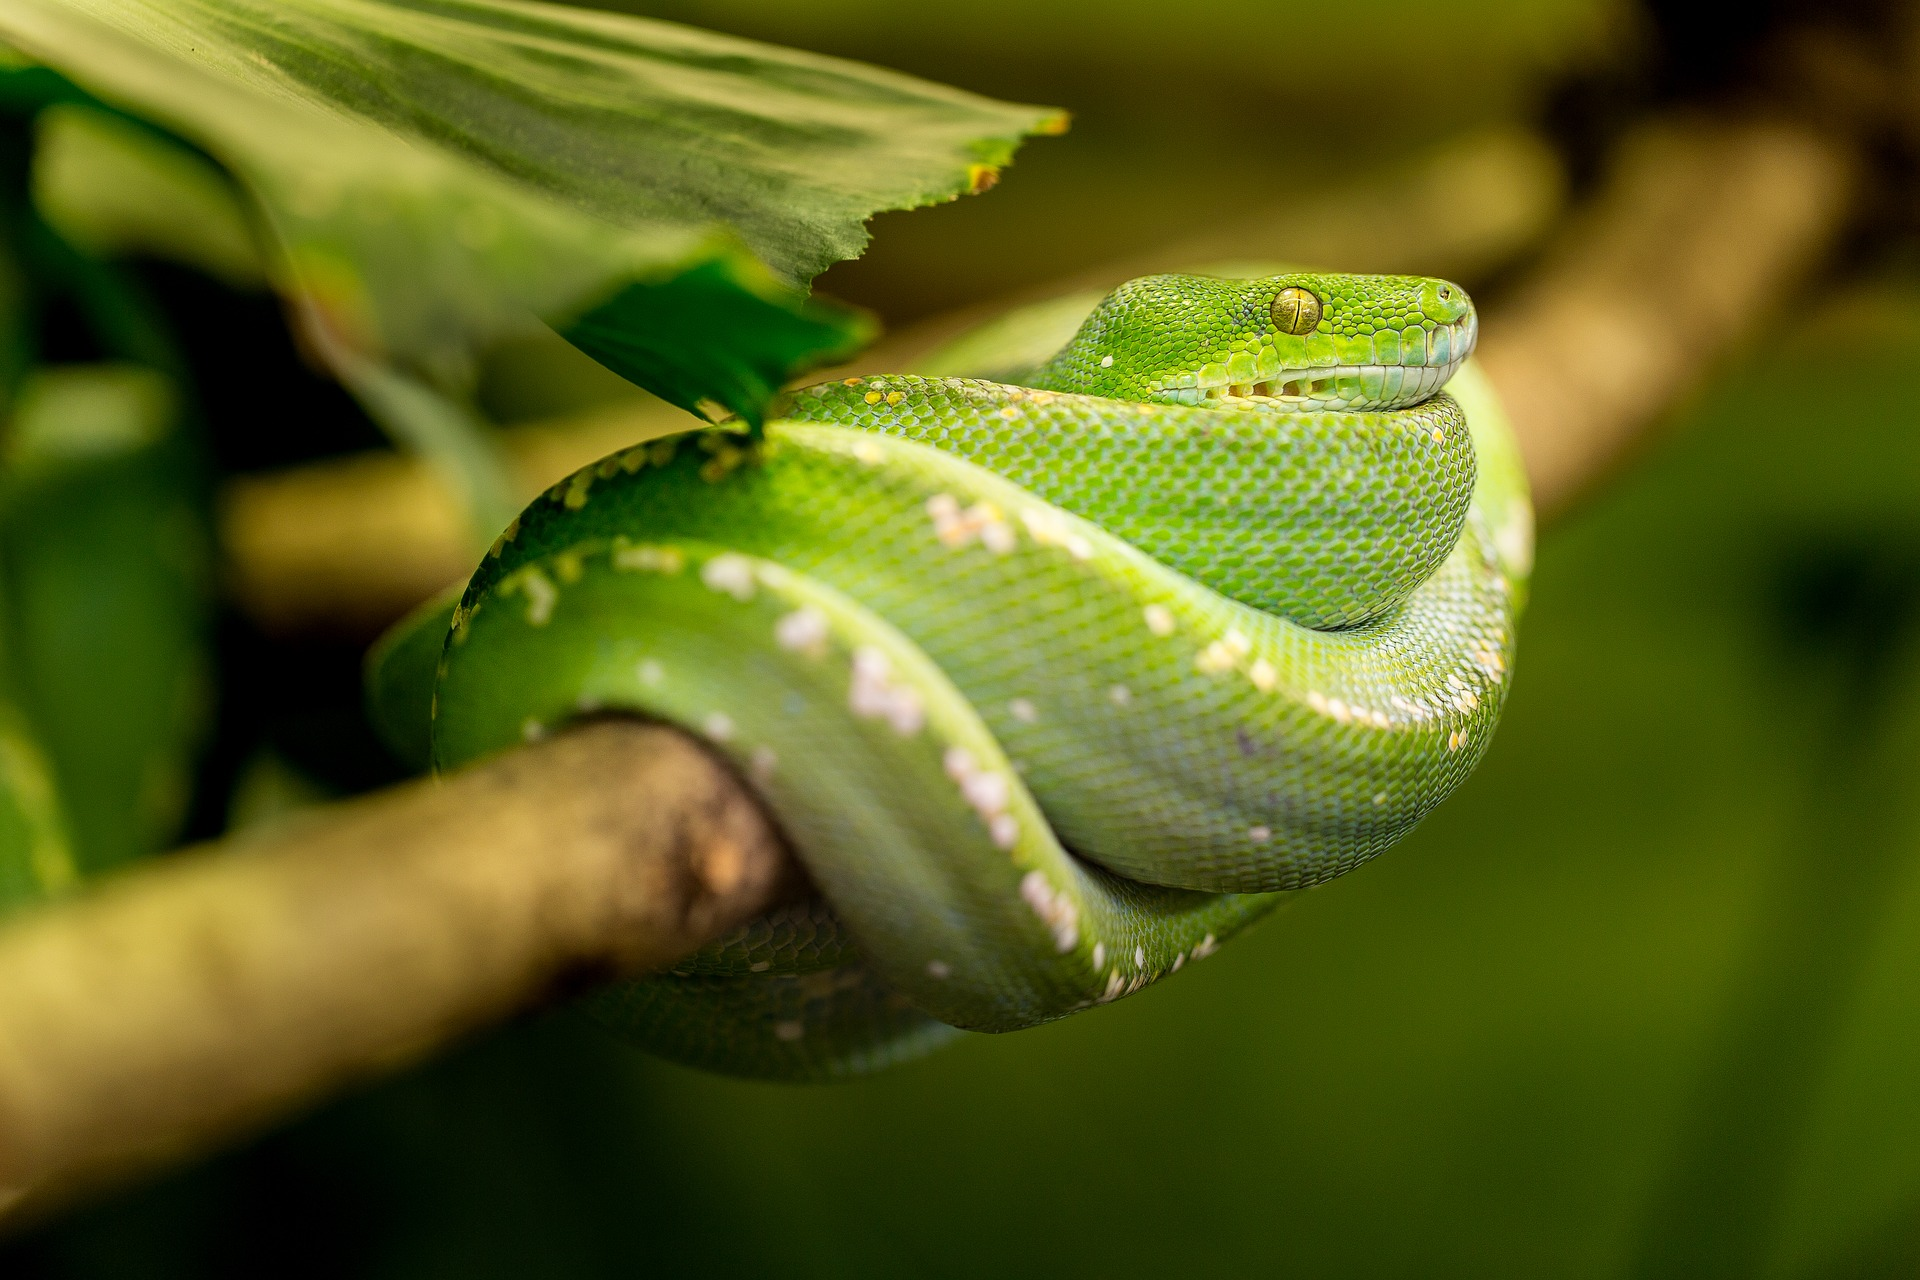
\includegraphics{24-python.jpg}

\justifying
The Python language is good for newcomers and experienced practitioners alike. Python is a highly extensible language with many add on modules available.
There is a collection known as \href{https://pypi.org/}{Pypi} where many of these Open Source\index{OpenSource} module projects are hosted. Python has a
fairly gentle learning curve, especially when compared to other languages. Python runs ``everywhere'', for all intents and purposes. With it's gentle
learning curve, it has become the go to language for Data Scientists, System Administrators, and yes, even DevSecOps folks like ourselves. For all these
reasons, Python makes a great addition to our toolbox.

\justifying
The goal of this chapter is not to teach you how to program with Python. There are many existing, well written resources already available on the Internet
that can help you with this. Our purpose here is derive repeatable patterns and best practices that can help us realize reusability and scalability in our projects. In other words, we will focus on some things that will get your projects up and running quickly.

\justifying
Consistently putting our files in the same places with the same naming convention becomes helpful as the number of projects we accumulate over the years
grows from the tens into the hundreds. This strategy can also help with code reuse across projects, as bits of codes can be quickly copied to new projects
or used to refresh existing projects with minimal refactoring.

\justifying
An item of note, Python3 is our only choice at this point. Python 2.x End of Life was January 1st, 2020.

\section{Local Development Environment}

\justifying
Support for modern operating systems is available, and installation of the necessary files to support Python is a relatively painless experience.

\markdownInput{../labs/24-python/lab-24-python-a.md}

\section{Python Virtual Environments}

\justifying
Temporary virtual environments allow us to confine the dependencies for our project to a temporary workspace.
This is preferable to installing project dependencies directly to a development workstation, as we may be
testing with modules that could corrupt the working configuration on the workstation.

\markdownInput{../labs/24-python/lab-24-python-b.md}

\section{Requirements Files}

\justifying
A requirements file lists the required Python modules needed to build and run any Python portions of our
project. We also add a check in the Makefile to verify the existence of the requirements.txt file.

\justifying
Some requirements are strictly intended to be part of the test harness, but are not needed for the application
proper. Using a separate file, such as tests/requirements-test.txt, makes this delineation clear to folks who are not familiar with the project.

\markdownInput{../labs/24-python/lab-24-python-c.md}

\section{The \_\_init\_\_.py File}

\justifying
We add this file to let the Python interpreter know that the directories the file is found in are a contiguous part of our Python project. Since module
imports and function definitions in this file are available to all the Python code files in the directory, we can use it to our advantage. For example, try
adding this quick and dirty logging function to src/\_\_init\_\_.py

\justifying
\begin{mybox}{\thetcbcounter: \_\_init\_\_.py}
  \lstinputlisting{code/24-python/init.py}
\end{mybox}

\section{Logging Framework}
\justifying
Now we can create a Python file ``src/logging.py'' and call the logger from within like so:

\begin{mybox}{\thetcbcounter: logging.py}
    \lstinputlisting{code/24-python/logtest.py}
\end{mybox}

\justifying
Check the results in the file /var/log/devsecops/devsecops.log.

\section{Logging Framework}

\justifying
We can create a file to define the characteristics of our logging mechanism.

\begin{mybox}{\thetcbcounter: logging.conf}
	\lstinputlisting{code/24-python/logging.conf}
\end{mybox}

\justifying
Now we can use this framework in the source files for our project.

\begin{mybox}{\thetcbcounter: logging}
	\lstinputlisting{code/24-python/logging-config}
\end{mybox}

\section{Python Directory Structure}
\justifying
Files and folders relevant to the Python portions of our project are shown in the diagram below.

\begin{figure}[!htb]
	\centering
	\chapter{Useful Python}

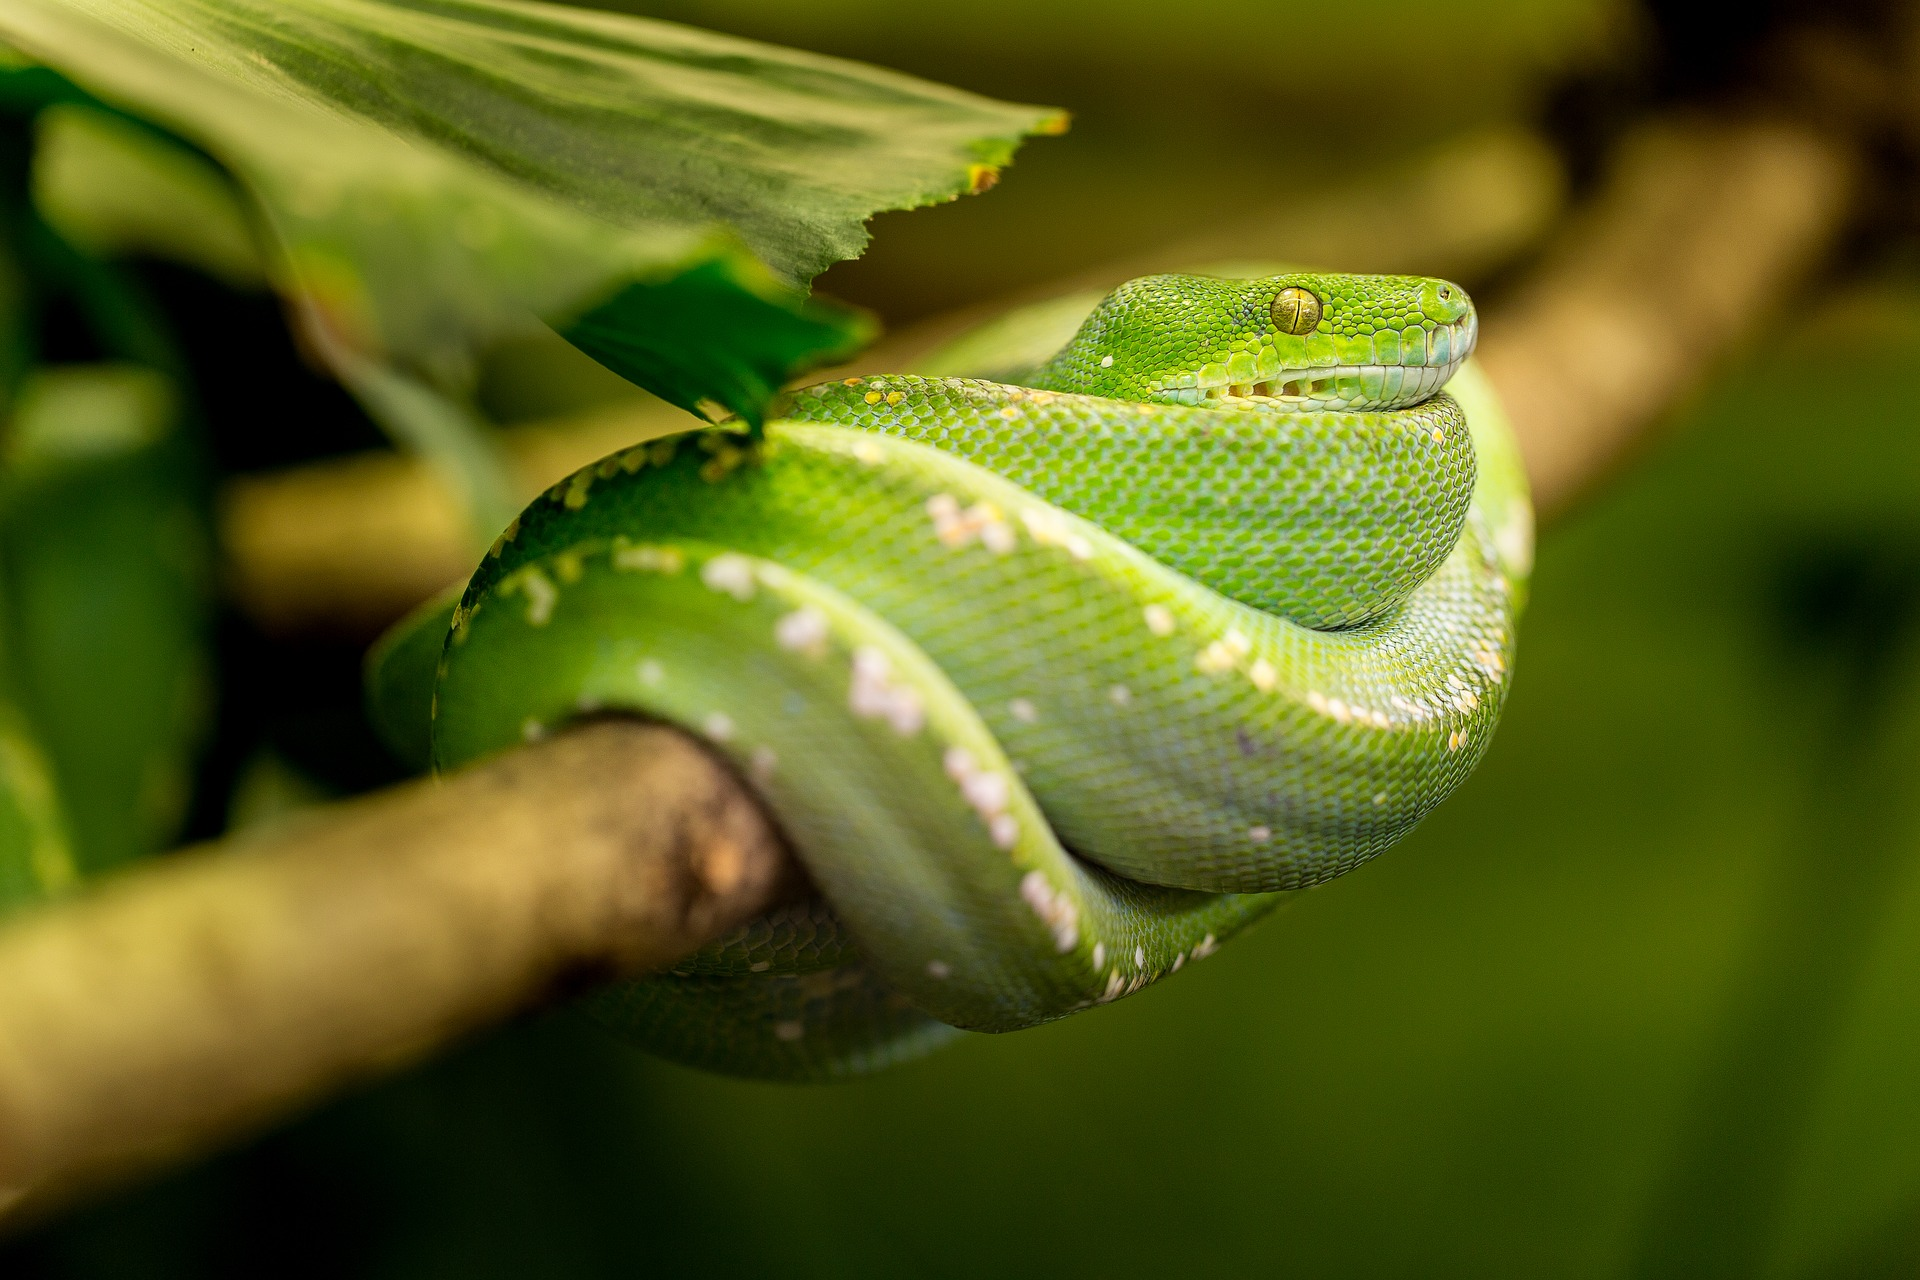
\includegraphics{24-python.jpg}

\justifying
The Python language is good for newcomers and experienced practitioners alike. Python is a highly extensible language with many add on modules available.
There is a collection known as \href{https://pypi.org/}{Pypi} where many of these Open Source\index{OpenSource} module projects are hosted. Python has a
fairly gentle learning curve, especially when compared to other languages. Python runs ``everywhere'', for all intents and purposes. With it's gentle
learning curve, it has become the go to language for Data Scientists, System Administrators, and yes, even DevSecOps folks like ourselves. For all these
reasons, Python makes a great addition to our toolbox.

\justifying
The goal of this chapter is not to teach you how to program with Python. There are many existing, well written resources already available on the Internet
that can help you with this. Our purpose here is derive repeatable patterns and best practices that can help us realize reusability and scalability in our projects. In other words, we will focus on some things that will get your projects up and running quickly.

\justifying
Consistently putting our files in the same places with the same naming convention becomes helpful as the number of projects we accumulate over the years
grows from the tens into the hundreds. This strategy can also help with code reuse across projects, as bits of codes can be quickly copied to new projects
or used to refresh existing projects with minimal refactoring.

\justifying
An item of note, Python3 is our only choice at this point. Python 2.x End of Life was January 1st, 2020.

\section{Local Development Environment}

\justifying
Support for modern operating systems is available, and installation of the necessary files to support Python is a relatively painless experience.

\markdownInput{../labs/24-python/lab-24-python-a.md}

\section{Python Virtual Environments}

\justifying
Temporary virtual environments allow us to confine the dependencies for our project to a temporary workspace.
This is preferable to installing project dependencies directly to a development workstation, as we may be
testing with modules that could corrupt the working configuration on the workstation.

\markdownInput{../labs/24-python/lab-24-python-b.md}

\section{Requirements Files}

\justifying
A requirements file lists the required Python modules needed to build and run any Python portions of our
project. We also add a check in the Makefile to verify the existence of the requirements.txt file.

\justifying
Some requirements are strictly intended to be part of the test harness, but are not needed for the application
proper. Using a separate file, such as tests/requirements-test.txt, makes this delineation clear to folks who are not familiar with the project.

\markdownInput{../labs/24-python/lab-24-python-c.md}

\section{The \_\_init\_\_.py File}

\justifying
We add this file to let the Python interpreter know that the directories the file is found in are a contiguous part of our Python project. Since module
imports and function definitions in this file are available to all the Python code files in the directory, we can use it to our advantage. For example, try
adding this quick and dirty logging function to src/\_\_init\_\_.py

\justifying
\begin{mybox}{\thetcbcounter: \_\_init\_\_.py}
  \lstinputlisting{code/24-python/init.py}
\end{mybox}

\section{Logging Framework}
\justifying
Now we can create a Python file ``src/logging.py'' and call the logger from within like so:

\begin{mybox}{\thetcbcounter: logging.py}
    \lstinputlisting{code/24-python/logtest.py}
\end{mybox}

\justifying
Check the results in the file /var/log/devsecops/devsecops.log.

\section{Logging Framework}

\justifying
We can create a file to define the characteristics of our logging mechanism.

\begin{mybox}{\thetcbcounter: logging.conf}
	\lstinputlisting{code/24-python/logging.conf}
\end{mybox}

\justifying
Now we can use this framework in the source files for our project.

\begin{mybox}{\thetcbcounter: logging}
	\lstinputlisting{code/24-python/logging-config}
\end{mybox}

\section{Python Directory Structure}
\justifying
Files and folders relevant to the Python portions of our project are shown in the diagram below.

\begin{figure}[!htb]
	\centering
	\chapter{Useful Python}

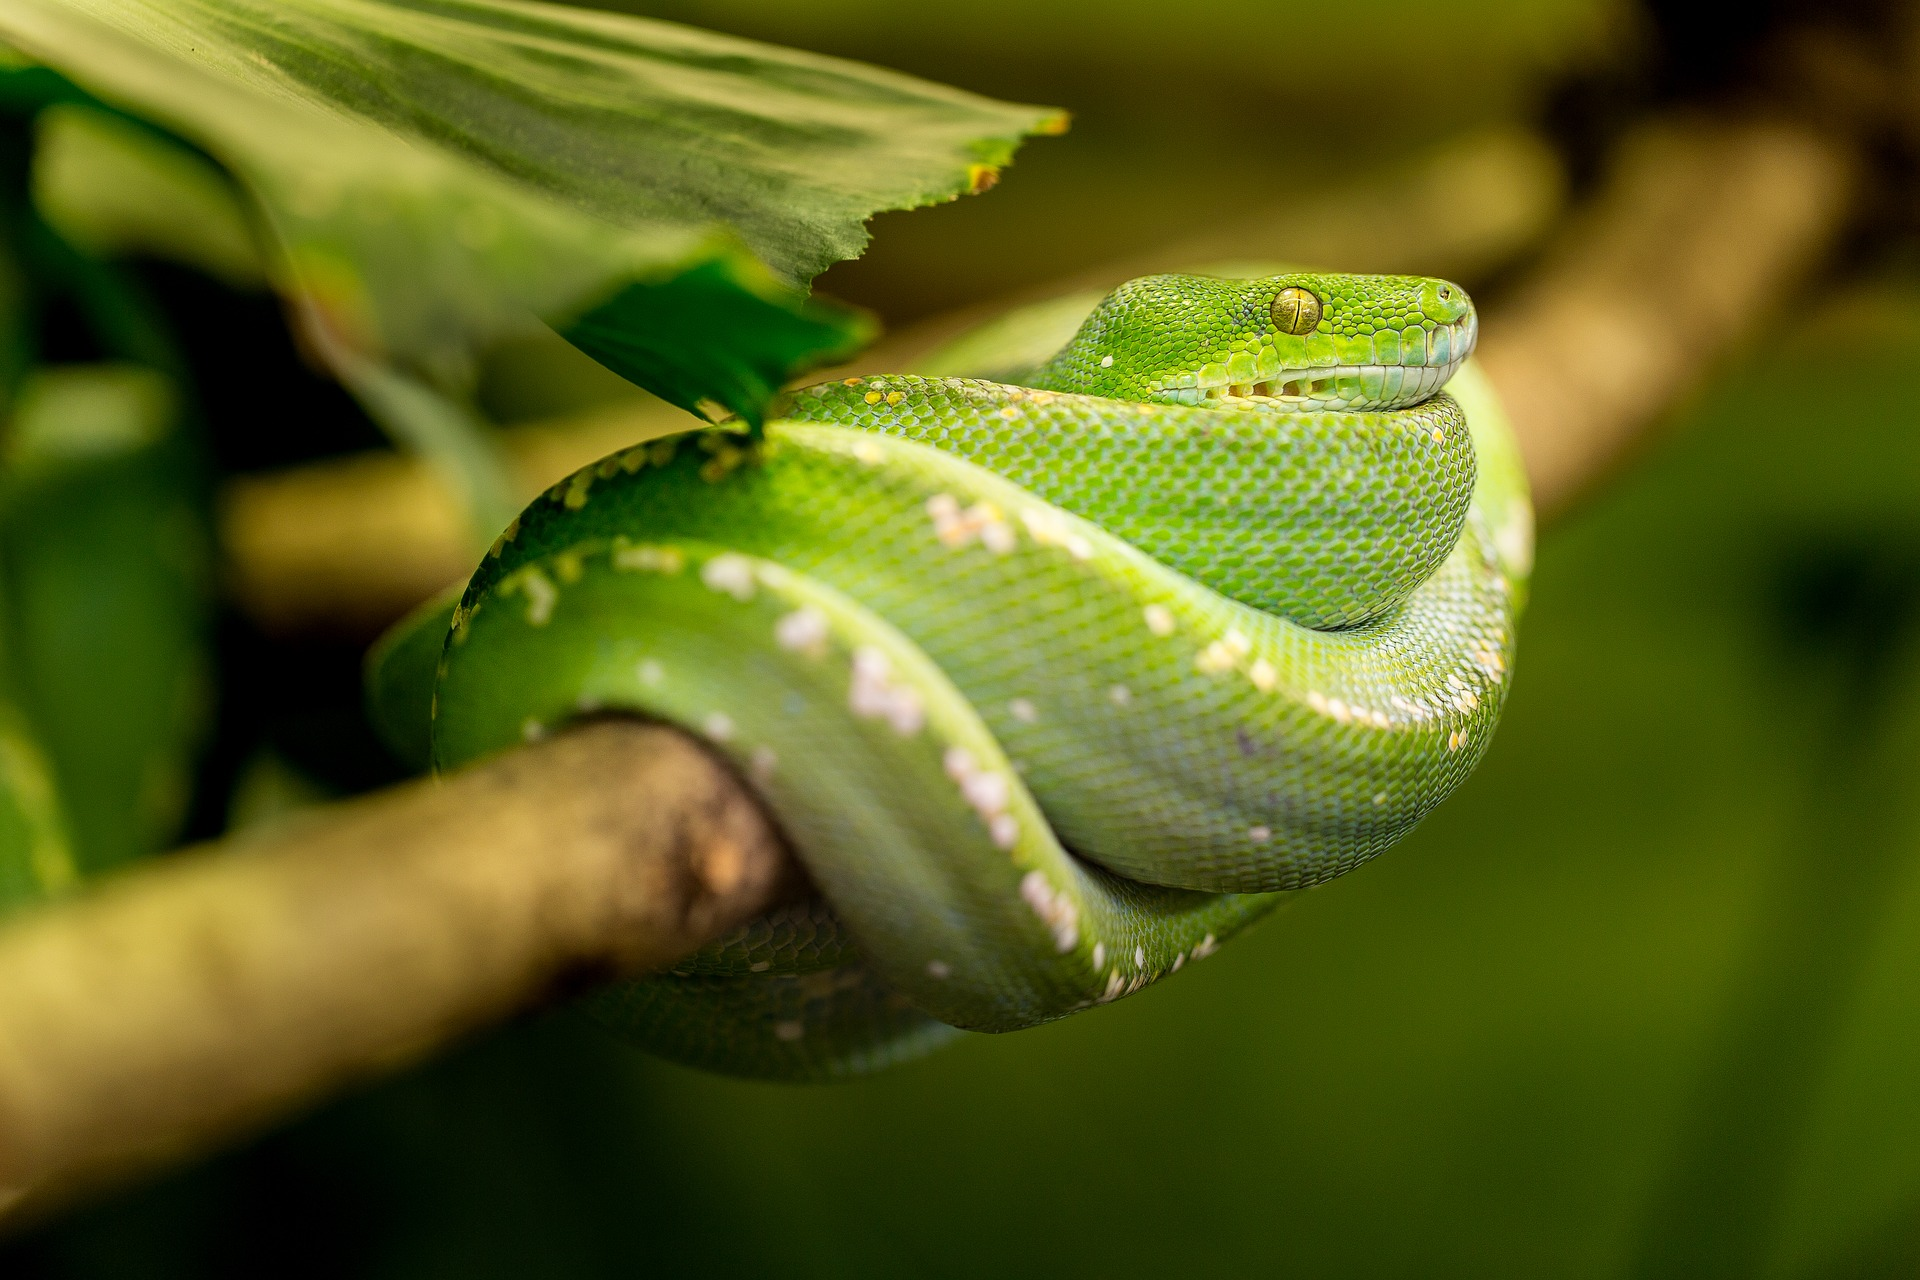
\includegraphics{24-python.jpg}

\justifying
The Python language is good for newcomers and experienced practitioners alike. Python is a highly extensible language with many add on modules available.
There is a collection known as \href{https://pypi.org/}{Pypi} where many of these Open Source\index{OpenSource} module projects are hosted. Python has a
fairly gentle learning curve, especially when compared to other languages. Python runs ``everywhere'', for all intents and purposes. With it's gentle
learning curve, it has become the go to language for Data Scientists, System Administrators, and yes, even DevSecOps folks like ourselves. For all these
reasons, Python makes a great addition to our toolbox.

\justifying
The goal of this chapter is not to teach you how to program with Python. There are many existing, well written resources already available on the Internet
that can help you with this. Our purpose here is derive repeatable patterns and best practices that can help us realize reusability and scalability in our projects. In other words, we will focus on some things that will get your projects up and running quickly.

\justifying
Consistently putting our files in the same places with the same naming convention becomes helpful as the number of projects we accumulate over the years
grows from the tens into the hundreds. This strategy can also help with code reuse across projects, as bits of codes can be quickly copied to new projects
or used to refresh existing projects with minimal refactoring.

\justifying
An item of note, Python3 is our only choice at this point. Python 2.x End of Life was January 1st, 2020.

\section{Local Development Environment}

\justifying
Support for modern operating systems is available, and installation of the necessary files to support Python is a relatively painless experience.

\markdownInput{../labs/24-python/lab-24-python-a.md}

\section{Python Virtual Environments}

\justifying
Temporary virtual environments allow us to confine the dependencies for our project to a temporary workspace.
This is preferable to installing project dependencies directly to a development workstation, as we may be
testing with modules that could corrupt the working configuration on the workstation.

\markdownInput{../labs/24-python/lab-24-python-b.md}

\section{Requirements Files}

\justifying
A requirements file lists the required Python modules needed to build and run any Python portions of our
project. We also add a check in the Makefile to verify the existence of the requirements.txt file.

\justifying
Some requirements are strictly intended to be part of the test harness, but are not needed for the application
proper. Using a separate file, such as tests/requirements-test.txt, makes this delineation clear to folks who are not familiar with the project.

\markdownInput{../labs/24-python/lab-24-python-c.md}

\section{The \_\_init\_\_.py File}

\justifying
We add this file to let the Python interpreter know that the directories the file is found in are a contiguous part of our Python project. Since module
imports and function definitions in this file are available to all the Python code files in the directory, we can use it to our advantage. For example, try
adding this quick and dirty logging function to src/\_\_init\_\_.py

\justifying
\begin{mybox}{\thetcbcounter: \_\_init\_\_.py}
  \lstinputlisting{code/24-python/init.py}
\end{mybox}

\section{Logging Framework}
\justifying
Now we can create a Python file ``src/logging.py'' and call the logger from within like so:

\begin{mybox}{\thetcbcounter: logging.py}
    \lstinputlisting{code/24-python/logtest.py}
\end{mybox}

\justifying
Check the results in the file /var/log/devsecops/devsecops.log.

\section{Logging Framework}

\justifying
We can create a file to define the characteristics of our logging mechanism.

\begin{mybox}{\thetcbcounter: logging.conf}
	\lstinputlisting{code/24-python/logging.conf}
\end{mybox}

\justifying
Now we can use this framework in the source files for our project.

\begin{mybox}{\thetcbcounter: logging}
	\lstinputlisting{code/24-python/logging-config}
\end{mybox}

\section{Python Directory Structure}
\justifying
Files and folders relevant to the Python portions of our project are shown in the diagram below.

\begin{figure}[!htb]
	\centering
	\input{dot/24-python.tex}
	\caption{Project directory and related files.}
	\label{pythonfiles}
\end{figure}

	\caption{Project directory and related files.}
	\label{pythonfiles}
\end{figure}

	\caption{Project directory and related files.}
	\label{pythonfiles}
\end{figure}

%\chapter{Nix}

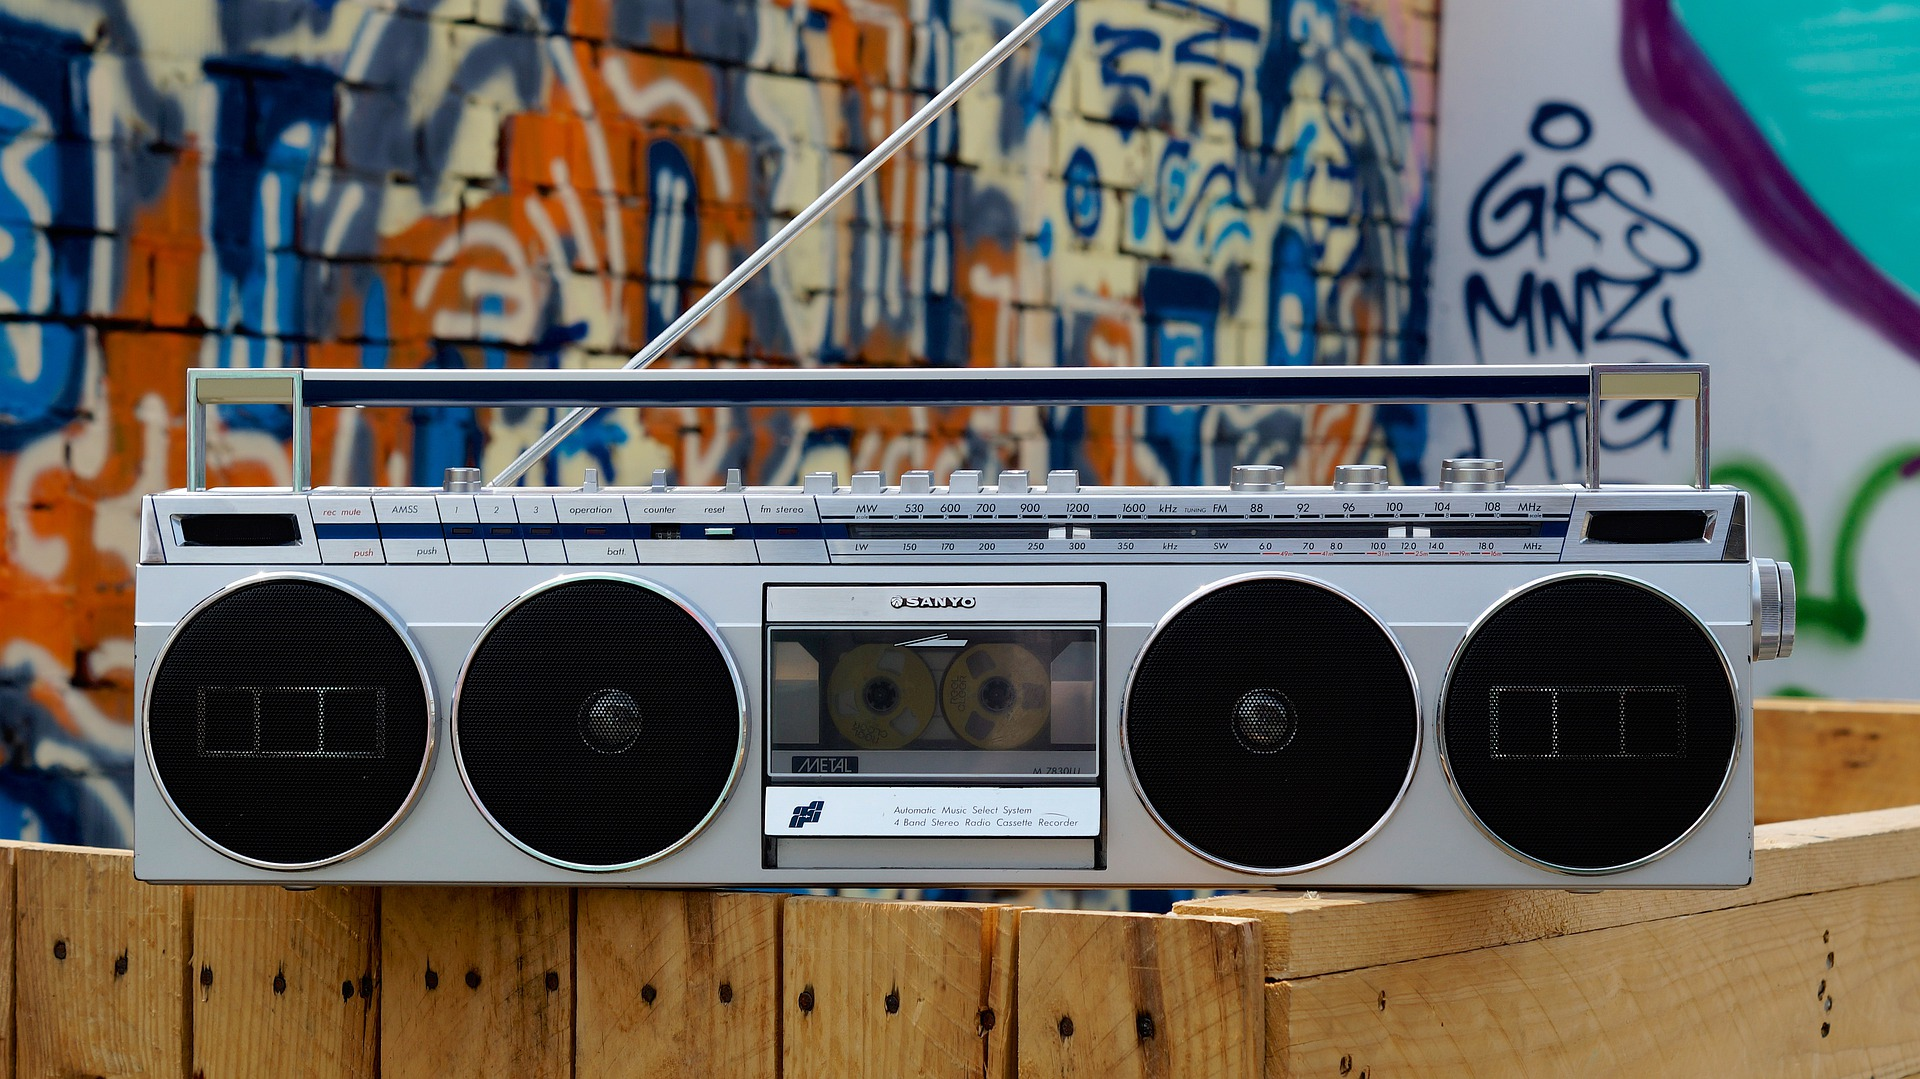
\includegraphics{25-nix.jpg}

\justifying
If you haven't tried Nix\index{Nix} yet, then now is a great time! The Nix ecosystem is all about
helping you reliably create ``nailed'' build environments. You as the developer get control over
the dependencies of a project, which increases  confidence in a high degree of fidelity around
expectations for your builds. Nix allows you to experiment in ways that don't break Nix itself,
or interfere with other projects on your system. Think ``virtualenv'' in Python,
but \href{https://github.com/NixOS/nixpkgs/tree/master/pkgs}{the nixpkgs repository}
allows you to mix and match support for multiple dependency version, languages, and more. There is a  \href{https://nixos.org/guides/how-nix-works.html}{well written introduction to Nix and how it works} available
on the web site for the project.

\justifying
Nix can be installed on your existing system, or used as a full operating system. For our purposes, we will
\href{https://nixos.org/download.html}{install nix to an existing environment} rather than go the full NixOs route.

\section{Setting up Nix as a Development Environment}

\justifying
In preparation for some labs using Nix, we will configure our development environment with nix-shell \href{https://nixos.wiki/wiki/Development_environment_with_nix-shell}{similar to the description at this web site}.

\section{Troubleshooting}

\justifying
Sometimes running nix-shell will fail with a ``Permission Denied'' error.

\begin{mybox}{\thetcbcounter: nix-shell error}
	\lstinputlisting{code/25-nix/nix-error.txt}
	\label{nixerr}
\end{mybox}

\justifying
To solve this error, you can type ``set -e NIX\_REMOTE'' in BASH shell.

\markdownInput{../labs/ch8/lab-8a.md}

\markdownInput{../labs/ch8/lab-8b.md}

\section{Nix Directory Structure}
\justifying
Files and folders relevant to the Nix portions of our project are shown in the diagram below.

\begin{figure}[!htb]
	\centering
	\chapter{Nix}

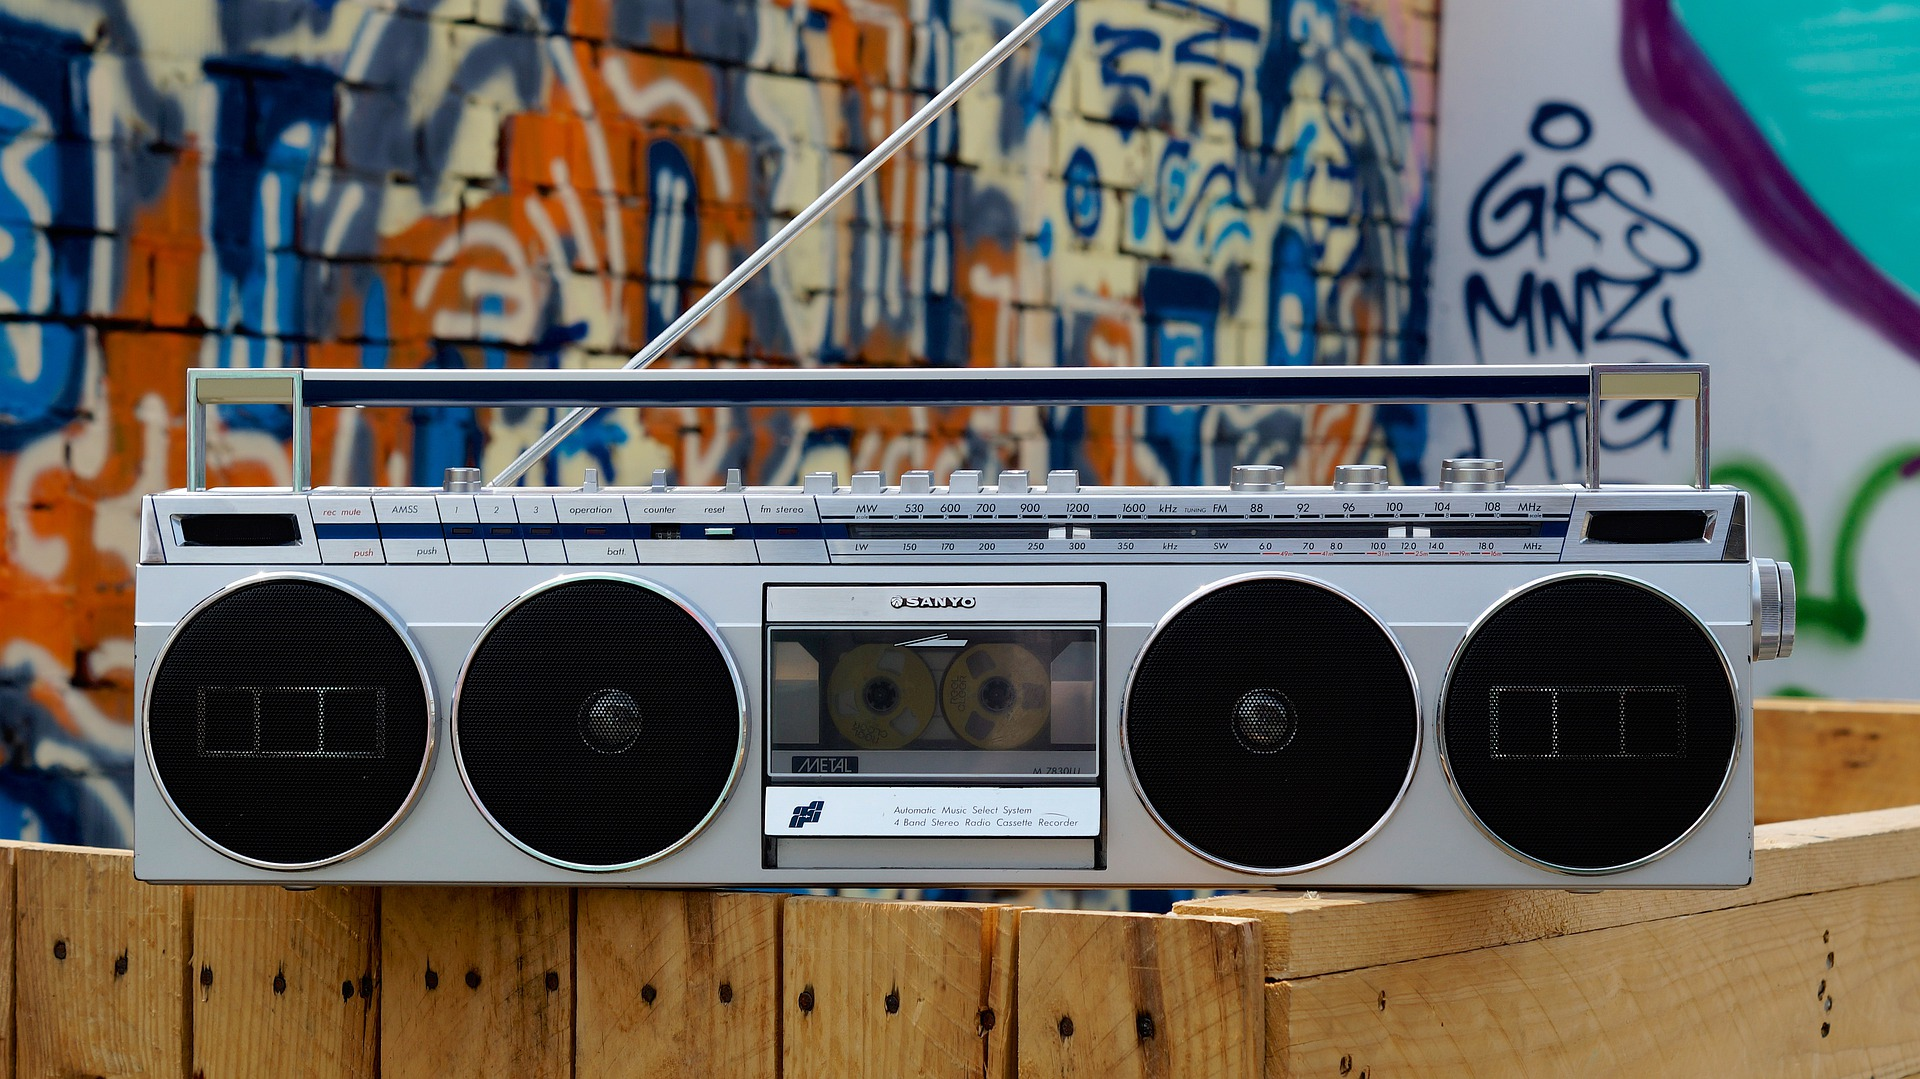
\includegraphics{25-nix.jpg}

\justifying
If you haven't tried Nix\index{Nix} yet, then now is a great time! The Nix ecosystem is all about
helping you reliably create ``nailed'' build environments. You as the developer get control over
the dependencies of a project, which increases  confidence in a high degree of fidelity around
expectations for your builds. Nix allows you to experiment in ways that don't break Nix itself,
or interfere with other projects on your system. Think ``virtualenv'' in Python,
but \href{https://github.com/NixOS/nixpkgs/tree/master/pkgs}{the nixpkgs repository}
allows you to mix and match support for multiple dependency version, languages, and more. There is a  \href{https://nixos.org/guides/how-nix-works.html}{well written introduction to Nix and how it works} available
on the web site for the project.

\justifying
Nix can be installed on your existing system, or used as a full operating system. For our purposes, we will
\href{https://nixos.org/download.html}{install nix to an existing environment} rather than go the full NixOs route.

\section{Setting up Nix as a Development Environment}

\justifying
In preparation for some labs using Nix, we will configure our development environment with nix-shell \href{https://nixos.wiki/wiki/Development_environment_with_nix-shell}{similar to the description at this web site}.

\section{Troubleshooting}

\justifying
Sometimes running nix-shell will fail with a ``Permission Denied'' error.

\begin{mybox}{\thetcbcounter: nix-shell error}
	\lstinputlisting{code/25-nix/nix-error.txt}
	\label{nixerr}
\end{mybox}

\justifying
To solve this error, you can type ``set -e NIX\_REMOTE'' in BASH shell.

\markdownInput{../labs/ch8/lab-8a.md}

\markdownInput{../labs/ch8/lab-8b.md}

\section{Nix Directory Structure}
\justifying
Files and folders relevant to the Nix portions of our project are shown in the diagram below.

\begin{figure}[!htb]
	\centering
	\chapter{Nix}

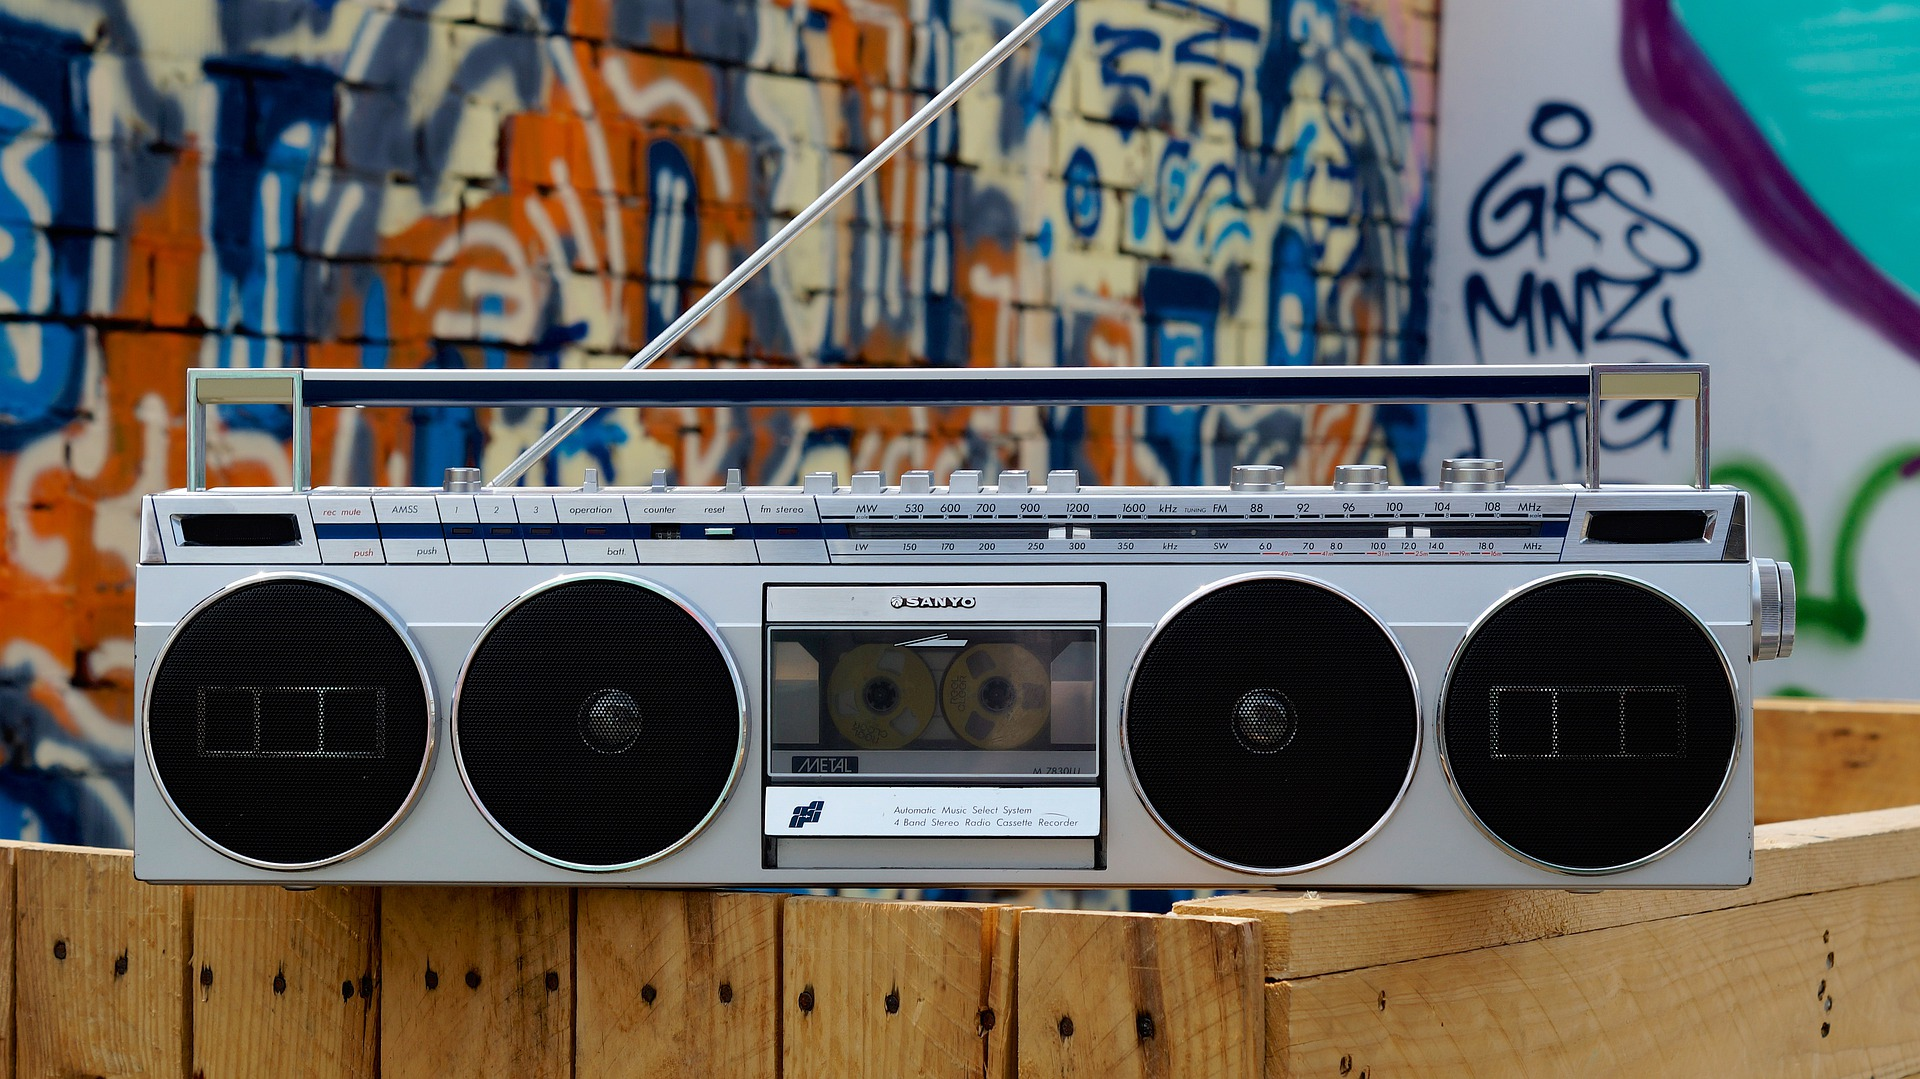
\includegraphics{25-nix.jpg}

\justifying
If you haven't tried Nix\index{Nix} yet, then now is a great time! The Nix ecosystem is all about
helping you reliably create ``nailed'' build environments. You as the developer get control over
the dependencies of a project, which increases  confidence in a high degree of fidelity around
expectations for your builds. Nix allows you to experiment in ways that don't break Nix itself,
or interfere with other projects on your system. Think ``virtualenv'' in Python,
but \href{https://github.com/NixOS/nixpkgs/tree/master/pkgs}{the nixpkgs repository}
allows you to mix and match support for multiple dependency version, languages, and more. There is a  \href{https://nixos.org/guides/how-nix-works.html}{well written introduction to Nix and how it works} available
on the web site for the project.

\justifying
Nix can be installed on your existing system, or used as a full operating system. For our purposes, we will
\href{https://nixos.org/download.html}{install nix to an existing environment} rather than go the full NixOs route.

\section{Setting up Nix as a Development Environment}

\justifying
In preparation for some labs using Nix, we will configure our development environment with nix-shell \href{https://nixos.wiki/wiki/Development_environment_with_nix-shell}{similar to the description at this web site}.

\section{Troubleshooting}

\justifying
Sometimes running nix-shell will fail with a ``Permission Denied'' error.

\begin{mybox}{\thetcbcounter: nix-shell error}
	\lstinputlisting{code/25-nix/nix-error.txt}
	\label{nixerr}
\end{mybox}

\justifying
To solve this error, you can type ``set -e NIX\_REMOTE'' in BASH shell.

\markdownInput{../labs/ch8/lab-8a.md}

\markdownInput{../labs/ch8/lab-8b.md}

\section{Nix Directory Structure}
\justifying
Files and folders relevant to the Nix portions of our project are shown in the diagram below.

\begin{figure}[!htb]
	\centering
	\input{dot/25-nix.tex}
	\caption{Nix directory and related files.}
	\label{nixfiles}
\end{figure}

	\caption{Nix directory and related files.}
	\label{nixfiles}
\end{figure}

	\caption{Nix directory and related files.}
	\label{nixfiles}
\end{figure}


\part{Security} % part 3
\chapter{Security Concepts}

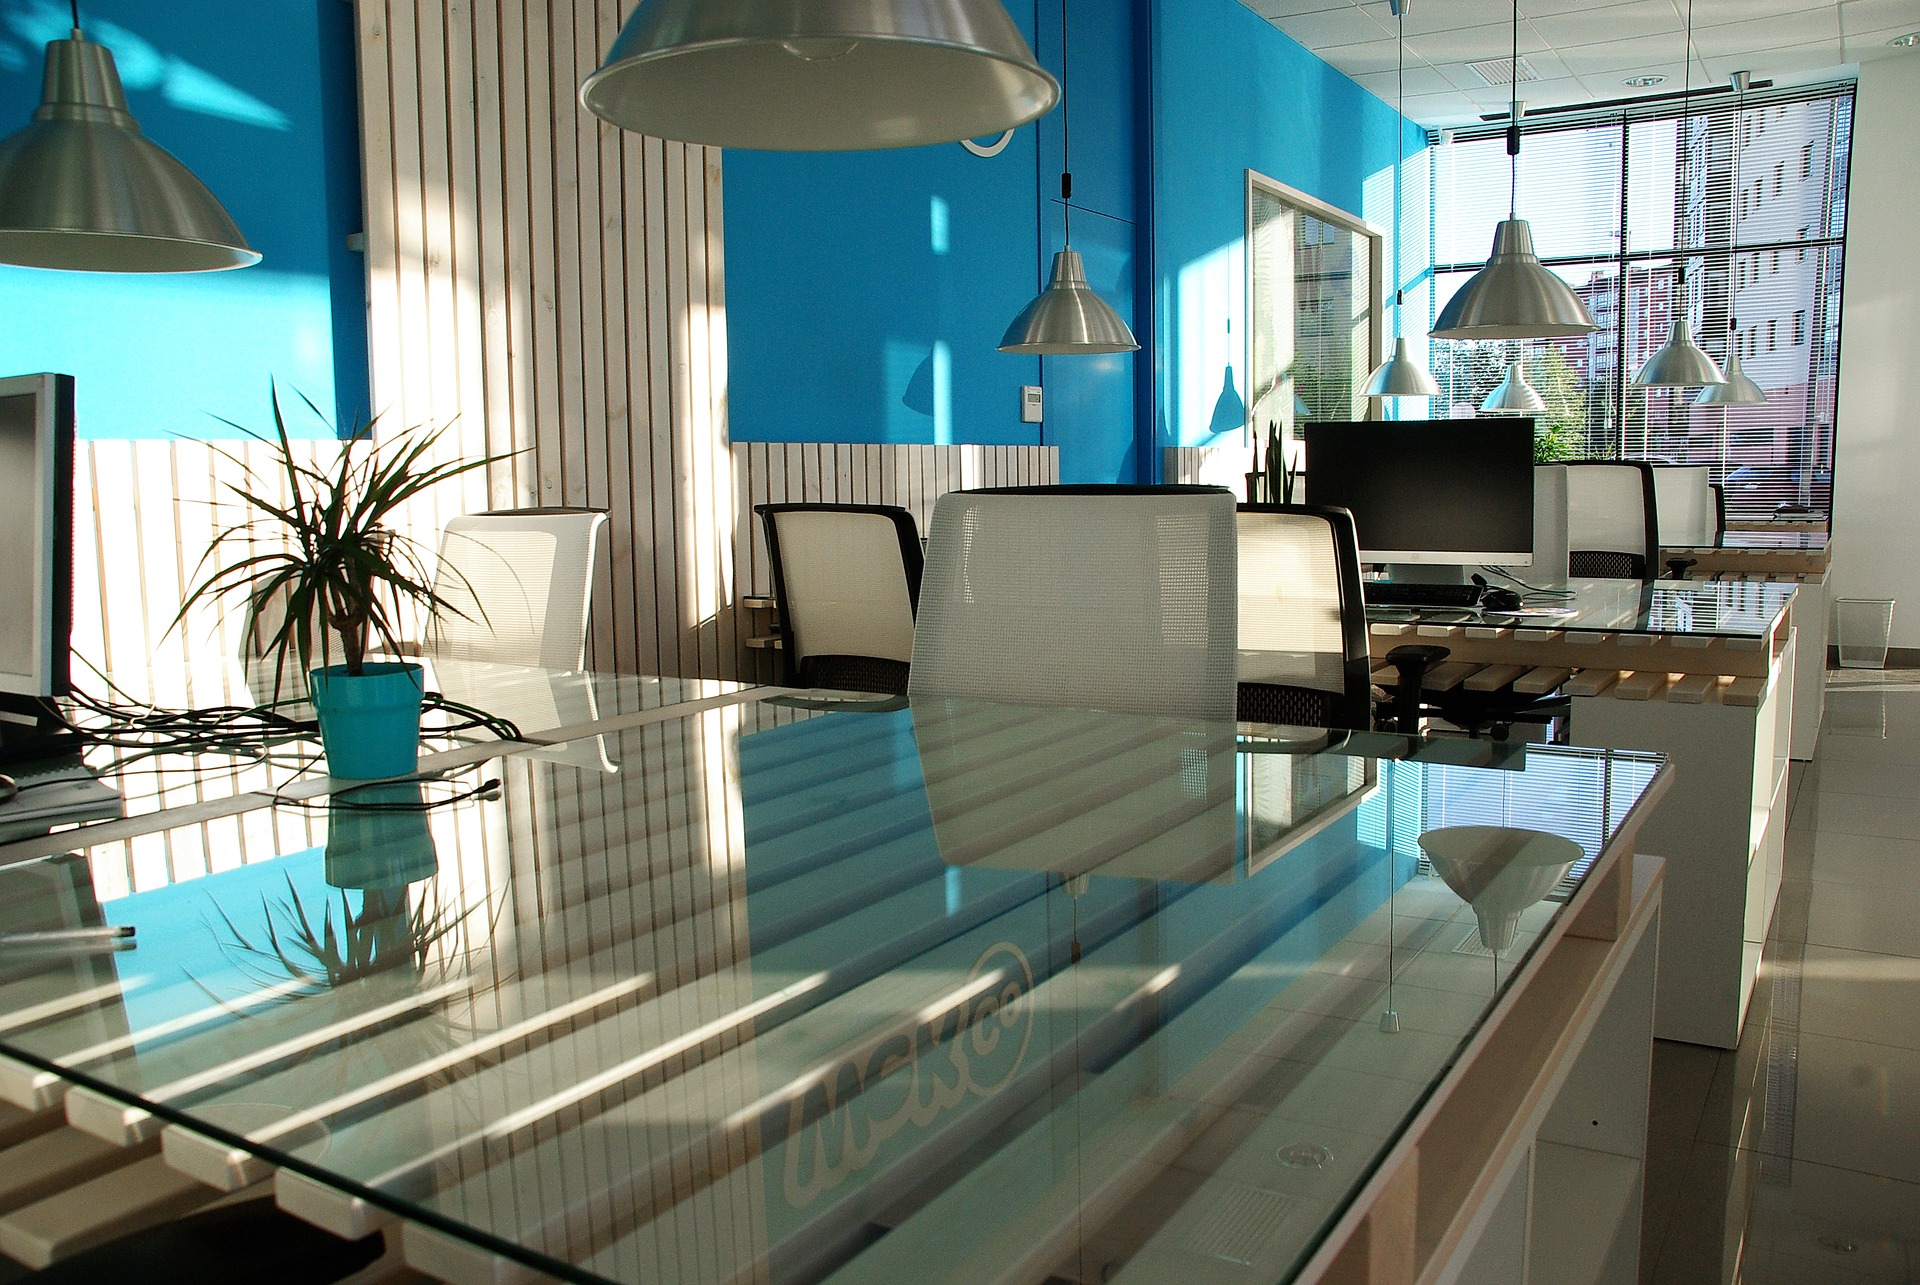
\includegraphics[scale=0.85]{images/office-space-1744803_1920.jpg}
\justify{}
Let's talk about some things.

\section{Security Mindedness}
\justify{}
This is the concept that security should be a part of all the things. 

\chapter{Security Testing}

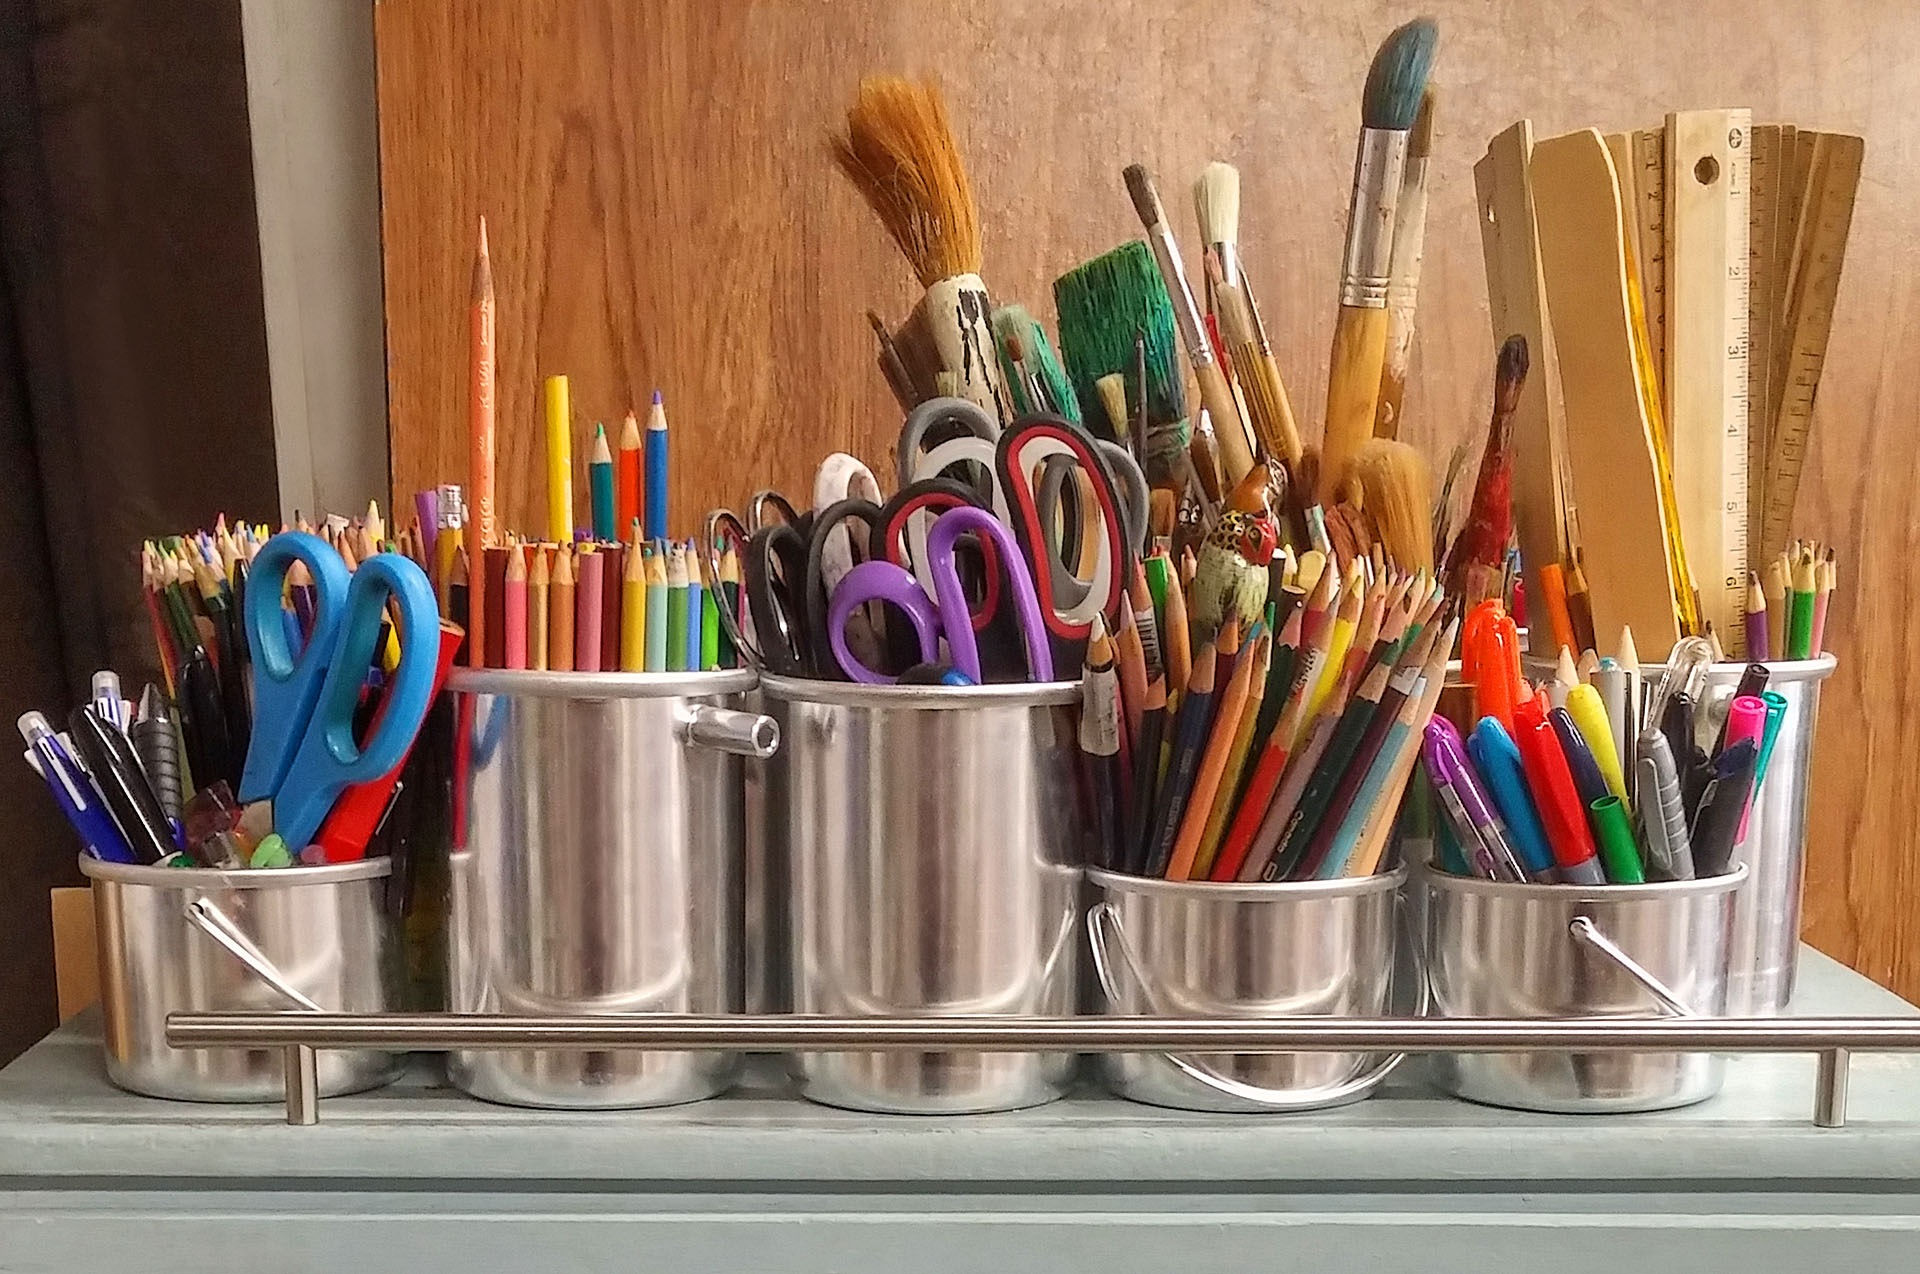
\includegraphics{31-security-testing.jpg}

This section is about things we can do to ensure we are driving out bugs and finding security issues as soon as possible in our product life cycle.

\markdownInput{../labs/31-security-testing/lab-31a-sec-test-setup.md}

\section{Code Scanning}

\markdownInput{../labs/31-security-testing/lab-31b-python-scanning.md}

% https://www.paloaltonetworks.com/cyberpedia/what-is-container-security

\markdownInput{../labs/ch4/lab-4c.md}

\section{Automated Security Scanning}

\justifying
There are many GitHub plugins that are free for single-user/non-commercial scenarios. a cursory search of the web of the
GitHub Marketplace will turn up many of these. Let's leave some of the
tedious work to the bots, allowing us to focus on our DevSecOps journey to the cloud!

\justifying
\begin{tabular}{| p{2.3cm}| p{4.5cm} | p{8.5cm} |}
    \hline
    \textbf{Tool}& \textbf{Purpose}& \textbf{Source} \\
    \hline
    bridgecrew & PR security scanner & web site \\
    \hline
\end{tabular}

\section{Validating Container Images}

\justifying
Lab with Hadolint and Trivy.

\markdownInput{../labs/31-security-testing/lab-31c-containers.md}

% lab - validating dependencies with ``safety''

\section{Directory Structure for Security Testing}

\justifying
Relevant files and folders related to our security testing framework are organized as seen below.

\begin{figure}[!htb]
    
\begin{tikzpicture}[>=latex,line join=bevel,]
  \pgfsetlinewidth{1bp}
%%
\pgfsetcolor{black}
  % Edge: devsecops -> tests
  \draw [->] (130.13bp,143.7bp) .. controls (124.5bp,135.47bp) and (117.65bp,125.48bp)  .. (105.73bp,108.1bp);
  % Edge: devsecops -> md
  \draw [->] (154.11bp,143.7bp) .. controls (159.87bp,135.47bp) and (166.86bp,125.48bp)  .. (179.03bp,108.1bp);
  % Edge: tests -> req
  \draw [->] (94.0bp,71.697bp) .. controls (94.0bp,63.983bp) and (94.0bp,54.712bp)  .. (94.0bp,36.104bp);
  % Node: devsecops
\begin{scope}
  \definecolor{strokecol}{rgb}{0.0,0.0,0.0};
  \pgfsetstrokecolor{strokecol}
  \draw (276.0bp,180.0bp) -- (273.0bp,184.0bp) -- (252.0bp,184.0bp) -- (249.0bp,180.0bp) -- (8.0bp,180.0bp) -- (8.0bp,144.0bp) -- (276.0bp,144.0bp) -- cycle;
  \draw (142.0bp,162.0bp) node {/home/devsecops/workspace/myproject};
\end{scope}
  % Node: tests
\begin{scope}
  \definecolor{strokecol}{rgb}{0.0,0.0,0.0};
  \pgfsetstrokecolor{strokecol}
  \draw (121.0bp,108.0bp) -- (118.0bp,112.0bp) -- (97.0bp,112.0bp) -- (94.0bp,108.0bp) -- (67.0bp,108.0bp) -- (67.0bp,72.0bp) -- (121.0bp,72.0bp) -- cycle;
  \draw (94.0bp,90.0bp) node {tests};
\end{scope}
  % Node: md
\begin{scope}
  \definecolor{strokecol}{rgb}{0.0,0.0,0.0};
  \pgfsetstrokecolor{strokecol}
  \draw (242.5bp,108.0bp) -- (139.5bp,108.0bp) -- (139.5bp,72.0bp) -- (242.5bp,72.0bp) -- cycle;
  \draw (191.0bp,90.0bp) node {SECURITY.md};
\end{scope}
  % Node: req
\begin{scope}
  \definecolor{strokecol}{rgb}{0.0,0.0,0.0};
  \pgfsetstrokecolor{strokecol}
  \draw (188.0bp,36.0bp) -- (0.0bp,36.0bp) -- (0.0bp,0.0bp) -- (188.0bp,0.0bp) -- cycle;
  \draw (94.0bp,18.0bp) node {requirements-security.txt};
\end{scope}
%
\end{tikzpicture}


    \caption{Security testing related files.}
    \label{sectest}
\end{figure}


%\part{Operations} % part 4
%\chapter{Continuous Integration \& Deployment}

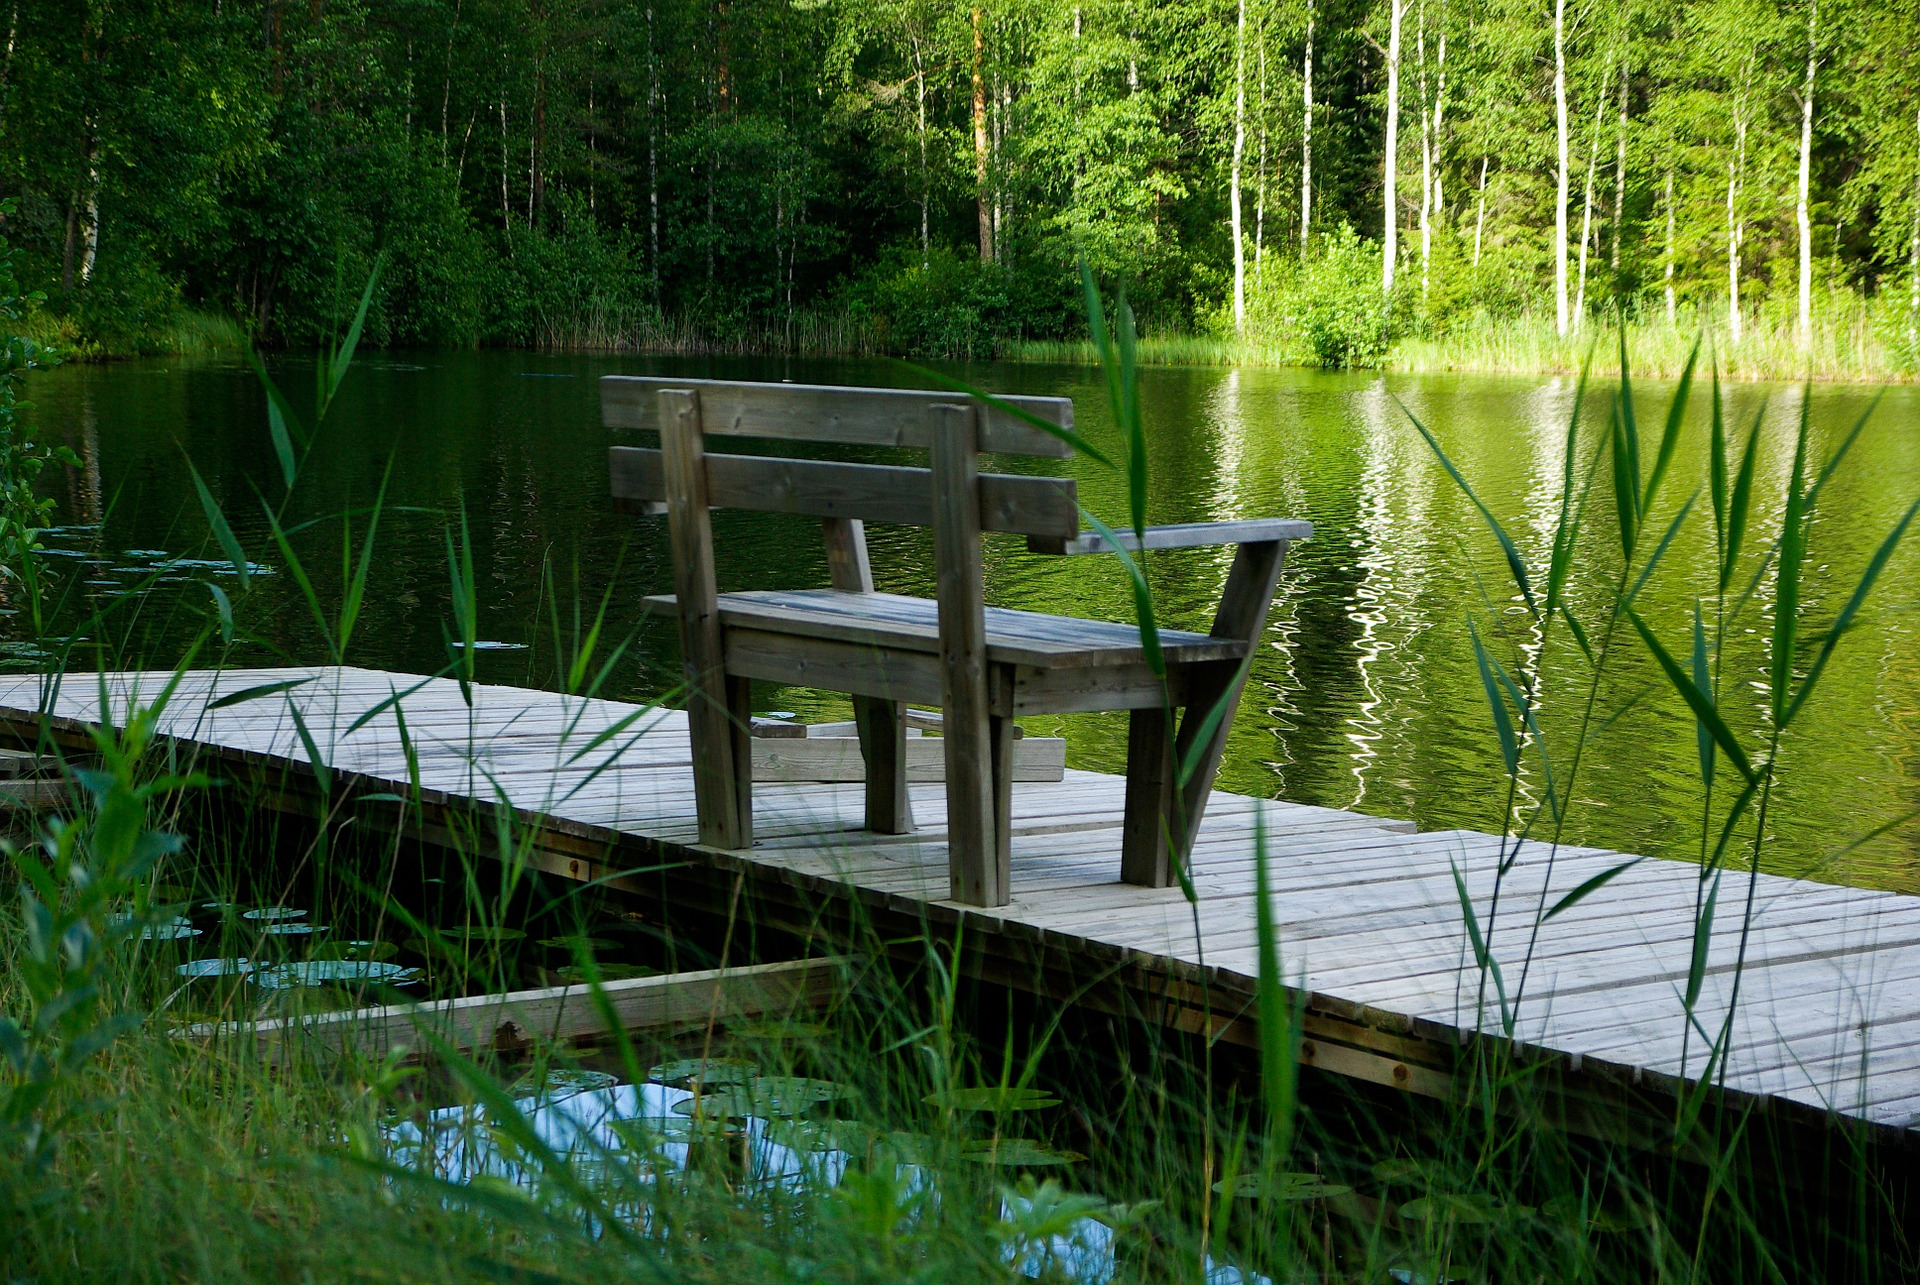
\includegraphics[scale=0.25]{41-about-ci-cd.jpg}

\justifying
Accommodations for Continuous Integration (CI) and Continuous Deployment
(CD) in our projects directly corresponds to our chances of success. One of the keys to
a successful build pipeline is speed. Time matters greatly as project size in terms of
code base and the number of folks pushing changes grows. It is entirely possible that
your CI may take hours, or even days. What is the impact of this when you have teams
of folks pushing new changes with a high frequency? We can easily find our testing
capacity has been outstripped.

\section{Linters}

\justifying
There are small programs for most (every?) language that you can run before
pushing your changes to GitHub that will catch syntactical and sometimes
even programmatic issues. Consider Python, which is very sensitive with
regard to indentation. You can programatically detect and even correct issues
before your work gets too far down the pipe. This is also a good way to
make sure folks are not committing dirty code to your repositories.

\justifying
Here are some of the linters I have found useful for languages I encounter
frequently.

\begin{table}[h]
	\begin{center}
		\begin{tabular}{| p{2.5cm}| p{2.5cm} | p{2.5cm} |}
			\hline
			\textbf{Language} & \textbf{Name} & \textbf{Source}\hfill                                                        \\
			Ansible           & ansible-lint  & python (pip install ansible-lint)                                      \\
			Markdown          & mdl           & ruby (gem install mdl)                                                 \\
			Puppet            & puppet-lint   & ruby (gem install puppet-lint)\url{http://puppet-lint.com/} \\
			Python            & pylint and flake8 & python \\
		\end{tabular}
	\end{center}
\end{table}



\section{GitHub Actions}

\justifying
GitHub Actions is a recent introduction to the github.com website that
lets you perform Continuous Integration on your repository, and Continuous
Deployment as desired.

\subsection{Docker}
\justifying
Let's see how we can leverage Actions to build the docker target in our
project. Save this YAML file under
codelab/.github/workflows/docker\_compose.yml to have GitHub Actions
execute our make docker target from our custom Makefile.

%\begin{mybox}{\thetcbcounter: A Makefile Target}
%	\lstinputlisting{code/makefile-target}
%\end{mybox}


\section{Python}
\justifying
Save this YAML file under codelab/.github/workflows/python.yml to have
GitHub Actions execute our make python target from our custom Makefile.

%\begin{mybox}{\thetcbcounter: Python GitHub action}
%	\lstinputlisting{code/makefile-target}
%\end{mybox}

\subsection{Packer}
\justifying
Save this YAML file under devsecops/.github/workflows/packer.yml to have
GitHub Actions validate and build our AMI image with Packer.

%\begin{mybox}{\thetcbcounter: AWS Debian host with packer}
%	\lstinputlisting{code/aws-debian-host.json}
%\end{mybox}

\subsection{Markdown}
\justifying
The following example YAML file illustrates how to validate GitHub
flavored Markdown text files using a GitHub Action.

%\begin{mybox}{\thetcbcounter: A GitHub Action for linting markdown files}
%	\lstinputlisting{code/makefile-target}
%\end{mybox}

\justifying
Note the designation of a configuration file named .markdownlint.json at
the top level of our repository. This JSON file is used to skip certain
checks by the markdownlint tool.

%\begin{mybox}{\thetcbcounter: The .markdownlint.json config file}
%	\lstinputlisting{code/makefile-target}
%\end{mybox}

\section{Circle CI}
\justifying
Circle CI\index{Circle CI} is a Continuous Integration service free for non-commercial
projects.

%\begin{mybox}{\thetcbcounter: A Circle CI configuration file}
%	\lstinputlisting{code/makefile-target}
%\end{mybox}

\section{Travis CI}

\justifying
Travis CI\index{Travis CI} is a hosted continuous integration service used to build and
test software projects hosted at GitHub and Bitbucket. They have a great
tutorial available if you care to dig a bit deeper.

\justifying
By enabling Travis CI integration through the GitHub Marketplace you
can integrate their scanners with your repository.

\subsubsection{Docker}

\justifying
You can test Docker containers in your CI/CD pipeline. As seen in the
following example I created a YAML file named .travis.yml to enable
automatic molecule testing of Ansible\index{Ansible} roles in Travis CI. I also set a
flag in the repo settings that prevent the PR from being merged until
Travis CI flags the build as passing.

%\begin{mybox}{\thetcbcounter: A Docker container test}
%	\lstinputlisting{code/makefile-target}
%\end{mybox}
\justifying
The contents of the requirements files and the example Ansible code is
available in the companion repo.


\subsection{Markdown}
\justifying
Save these lines to a file named .travis.yml to scan all the markdown files in your
repository.

%begin{mybox}{\thetcbcounter: A Travis config file}
%	\lstinputlisting{code/makefile-target}
%\end{mybox}

\justifying
You can also create an .mdlrc file to give mdl direction on what to scan for.

%\begin{mybox}{\thetcbcounter: A Markdown lint config file}
%	\lstinputlisting{code/makefile-target}
%\end{mybox}

\clearpage

\section{Directory Structure}

\justifying
Relevant folders and files related to our build pipeline are shown below. The users
home directory
and workspace subdirectory is implied and removed from the diagram for clarity.

\begin{figure}[!htb]
	
\begin{tikzpicture}[>=latex,line join=bevel,]
  \pgfsetlinewidth{1bp}
%%
\pgfsetcolor{black}
  % Edge: framework -> dotgh
  \draw [->] (95.919bp,144.33bp) .. controls (117.02bp,162.13bp) and (151.1bp,189.03bp)  .. (184.0bp,207.0bp) .. controls (194.07bp,212.5bp) and (205.5bp,217.37bp)  .. (225.81bp,224.87bp);
  % Edge: framework -> dotcircleci
  \draw [->] (135.35bp,144.06bp) .. controls (160.62bp,151.61bp) and (189.41bp,160.23bp)  .. (222.3bp,170.07bp);
  % Edge: framework -> dottr
  \draw [->] (148.16bp,126.0bp) .. controls (164.99bp,126.0bp) and (182.65bp,126.0bp)  .. (208.94bp,126.0bp);
  % Edge: framework -> mdlrc
  \draw [->] (135.35bp,107.94bp) .. controls (162.44bp,99.842bp) and (193.57bp,90.528bp)  .. (227.06bp,80.507bp);
  % Edge: framework -> mdjson
  \draw [->] (95.919bp,107.67bp) .. controls (117.02bp,89.868bp) and (151.1bp,62.975bp)  .. (184.0bp,45.0bp) .. controls (187.0bp,43.36bp) and (190.12bp,41.776bp)  .. (202.43bp,36.133bp);
  % Edge: dotgh -> workflows
  \draw [->] (287.33bp,234.0bp) .. controls (306.56bp,234.0bp) and (332.12bp,234.0bp)  .. (365.0bp,234.0bp);
  % Edge: workflows -> dcy
  \draw [->] (433.91bp,252.13bp) .. controls (449.27bp,263.45bp) and (470.12bp,277.77bp)  .. (490.0bp,288.0bp) .. controls (493.26bp,289.68bp) and (496.64bp,291.3bp)  .. (509.32bp,296.86bp);
  % Edge: workflows -> py
  \draw [->] (454.2bp,241.74bp) .. controls (471.05bp,244.72bp) and (490.51bp,248.17bp)  .. (518.5bp,253.12bp);
  % Edge: workflows -> pyyml
  \draw [->] (454.2bp,226.26bp) .. controls (470.9bp,223.31bp) and (490.17bp,219.89bp)  .. (517.97bp,214.97bp);
  % Edge: workflows -> mdy
  \draw [->] (440.67bp,215.75bp) .. controls (445.18bp,212.89bp) and (449.74bp,209.91bp)  .. (454.0bp,207.0bp) .. controls (470.51bp,195.72bp) and (472.44bp,189.57bp)  .. (490.0bp,180.0bp) .. controls (493.06bp,178.33bp) and (496.24bp,176.73bp)  .. (508.79bp,171.03bp);
  % Edge: dotcircleci -> cy
  \draw [->] (290.64bp,180.0bp) .. controls (309.82bp,180.0bp) and (334.41bp,180.0bp)  .. (366.24bp,180.0bp);
  % Node: framework
\begin{scope}
  \definecolor{strokecol}{rgb}{0.0,0.0,0.0};
  \pgfsetstrokecolor{strokecol}
  \draw (148.0bp,144.0bp) -- (145.0bp,148.0bp) -- (124.0bp,148.0bp) -- (121.0bp,144.0bp) -- (0.0bp,144.0bp) -- (0.0bp,108.0bp) -- (148.0bp,108.0bp) -- cycle;
  \draw (74.0bp,126.0bp) node {devsecops\_tactical};
\end{scope}
  % Node: dotgh
\begin{scope}
  \definecolor{strokecol}{rgb}{0.0,0.0,0.0};
  \pgfsetstrokecolor{strokecol}
  \draw (287.0bp,252.0bp) -- (284.0bp,256.0bp) -- (263.0bp,256.0bp) -- (260.0bp,252.0bp) -- (226.0bp,252.0bp) -- (226.0bp,216.0bp) -- (287.0bp,216.0bp) -- cycle;
  \draw (256.5bp,234.0bp) node {.github};
\end{scope}
  % Node: dotcircleci
\begin{scope}
  \definecolor{strokecol}{rgb}{0.0,0.0,0.0};
  \pgfsetstrokecolor{strokecol}
  \draw (290.5bp,198.0bp) -- (287.5bp,202.0bp) -- (266.5bp,202.0bp) -- (263.5bp,198.0bp) -- (222.5bp,198.0bp) -- (222.5bp,162.0bp) -- (290.5bp,162.0bp) -- cycle;
  \draw (256.5bp,180.0bp) node {.circleci};
\end{scope}
  % Node: dottr
\begin{scope}
  \definecolor{strokecol}{rgb}{0.0,0.0,0.0};
  \pgfsetstrokecolor{strokecol}
  \draw (304.0bp,144.0bp) -- (209.0bp,144.0bp) -- (209.0bp,108.0bp) -- (304.0bp,108.0bp) -- cycle;
  \draw (256.5bp,126.0bp) node {.travis.yml};
\end{scope}
  % Node: mdlrc
\begin{scope}
  \definecolor{strokecol}{rgb}{0.0,0.0,0.0};
  \pgfsetstrokecolor{strokecol}
  \draw (285.5bp,90.0bp) -- (227.5bp,90.0bp) -- (227.5bp,54.0bp) -- (285.5bp,54.0bp) -- cycle;
  \draw (256.5bp,72.0bp) node {.mdlrc};
\end{scope}
  % Node: mdjson
\begin{scope}
  \definecolor{strokecol}{rgb}{0.0,0.0,0.0};
  \pgfsetstrokecolor{strokecol}
  \draw (329.0bp,36.0bp) -- (184.0bp,36.0bp) -- (184.0bp,0.0bp) -- (329.0bp,0.0bp) -- cycle;
  \draw (256.5bp,18.0bp) node {.markdownlint.json};
\end{scope}
  % Node: workflows
\begin{scope}
  \definecolor{strokecol}{rgb}{0.0,0.0,0.0};
  \pgfsetstrokecolor{strokecol}
  \draw (454.0bp,252.0bp) -- (451.0bp,256.0bp) -- (430.0bp,256.0bp) -- (427.0bp,252.0bp) -- (365.0bp,252.0bp) -- (365.0bp,216.0bp) -- (454.0bp,216.0bp) -- cycle;
  \draw (409.5bp,234.0bp) node {workflows};
\end{scope}
  % Node: dcy
\begin{scope}
  \definecolor{strokecol}{rgb}{0.0,0.0,0.0};
  \pgfsetstrokecolor{strokecol}
  \draw (638.0bp,333.0bp) -- (490.0bp,333.0bp) -- (490.0bp,297.0bp) -- (638.0bp,297.0bp) -- cycle;
  \draw (564.0bp,315.0bp) node {docker\_compose.yml};
\end{scope}
  % Node: py
\begin{scope}
  \definecolor{strokecol}{rgb}{0.0,0.0,0.0};
  \pgfsetstrokecolor{strokecol}
  \draw (609.5bp,279.0bp) -- (518.5bp,279.0bp) -- (518.5bp,243.0bp) -- (609.5bp,243.0bp) -- cycle;
  \draw (564.0bp,261.0bp) node {packer.yml};
\end{scope}
  % Node: pyyml
\begin{scope}
  \definecolor{strokecol}{rgb}{0.0,0.0,0.0};
  \pgfsetstrokecolor{strokecol}
  \draw (610.0bp,225.0bp) -- (518.0bp,225.0bp) -- (518.0bp,189.0bp) -- (610.0bp,189.0bp) -- cycle;
  \draw (564.0bp,207.0bp) node {python.yml};
\end{scope}
  % Node: mdy
\begin{scope}
  \definecolor{strokecol}{rgb}{0.0,0.0,0.0};
  \pgfsetstrokecolor{strokecol}
  \draw (619.0bp,171.0bp) -- (509.0bp,171.0bp) -- (509.0bp,135.0bp) -- (619.0bp,135.0bp) -- cycle;
  \draw (564.0bp,153.0bp) node {markdown.yml};
\end{scope}
  % Node: cy
\begin{scope}
  \definecolor{strokecol}{rgb}{0.0,0.0,0.0};
  \pgfsetstrokecolor{strokecol}
  \draw (452.5bp,198.0bp) -- (366.5bp,198.0bp) -- (366.5bp,162.0bp) -- (452.5bp,162.0bp) -- cycle;
  \draw (409.5bp,180.0bp) node {config.yml};
\end{scope}
%
\end{tikzpicture}


	\caption{CI/CD related files and folders.}
\label{cicdfiles}
\end{figure}

%\chapter{Infrastructure}

\justifying
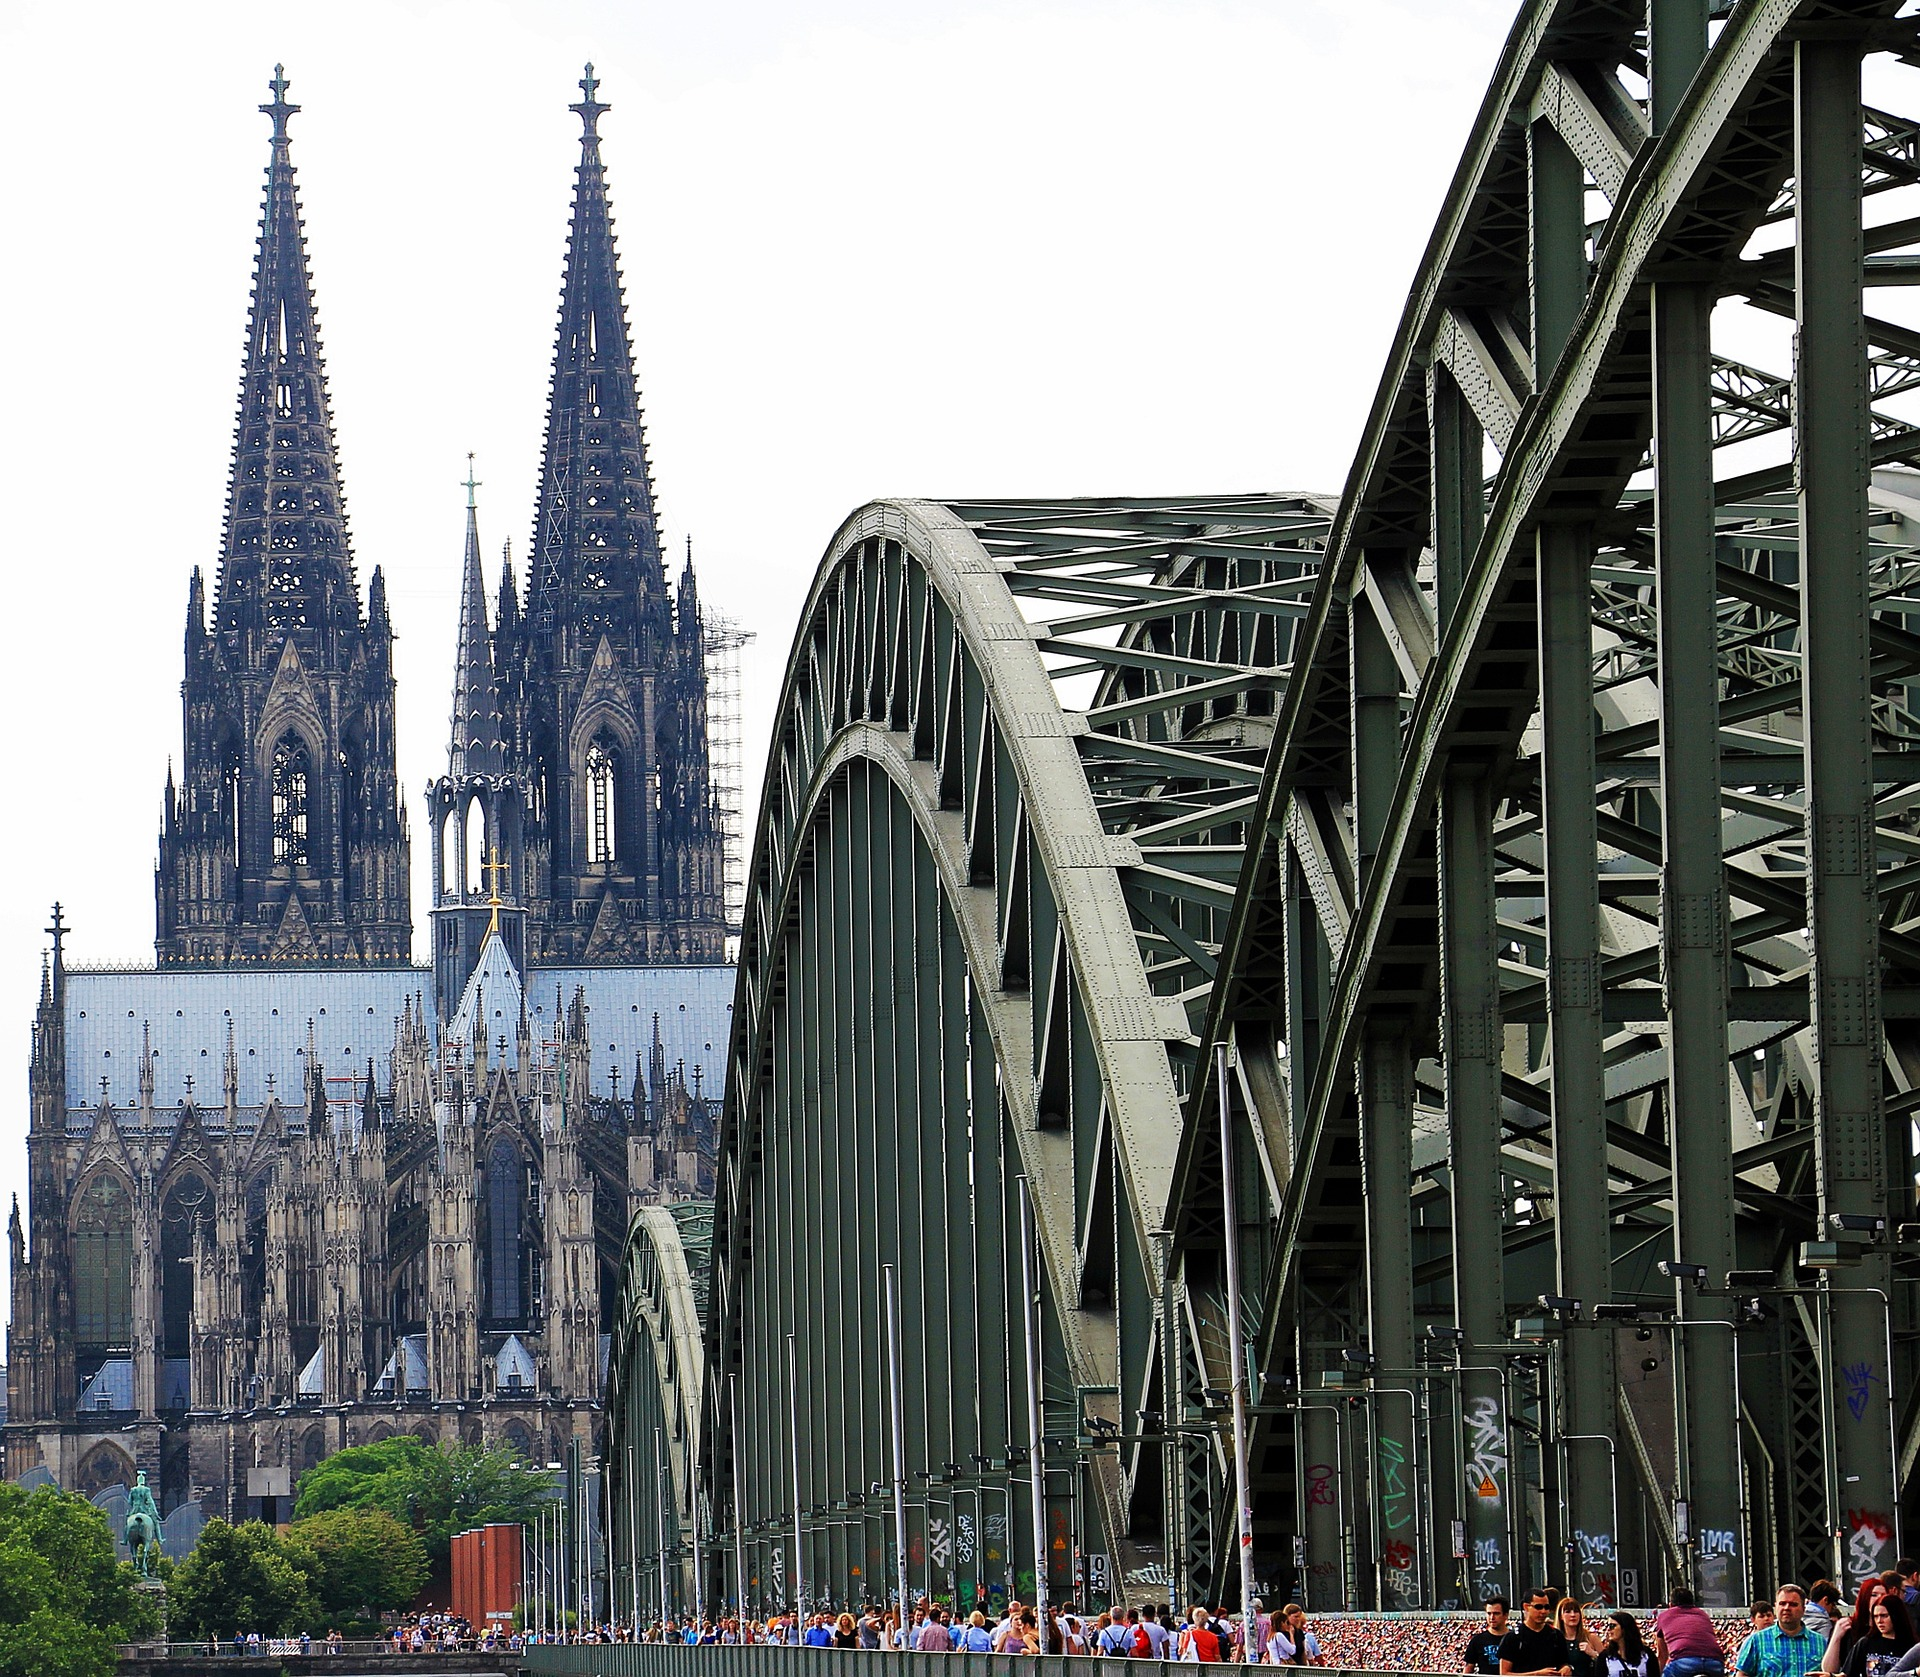
\includegraphics{42-infrastructure.jpg}

\justifying
Software Infrastructure and Platforms are the foundations upon which our
scripts, code, and projects are founded. Infrastructure comprises the
base upon which our containers rest, and the connectivity that allows us
to communicate with them and them with each other.

\justifying
This chapter details our ability to quickly and uniformly stand up and
tear down virtual domains and networks to connect our containers and
route their workloads. We will look at some popular cloud computing
providers to prepare to explore ways we can leverage them to our
benefit.

\justifying
A Public Cloud Provider is a company that offers to host our containerized
projects and virtual infrastructure so we don't have to do it ourselves.

\justifying
The virtual resources we subscribe to will be distributed across cloud
provider hardware in data centers around the world with very little
oversight or interaction from us. For example, we can choose a Region of
the world for our server instance to exist in, but we don't need to
worry about which machine or rack it's in, or even where the data center
is located.

\section{Amazon Web Services (AWS)}

%\justifying
%Consider \fig{aws} which illustrates the connectivity of a basic
%project using Amazon Web Services (AWS)\index{Amazon Web Services}.

%\begin{figure}
%  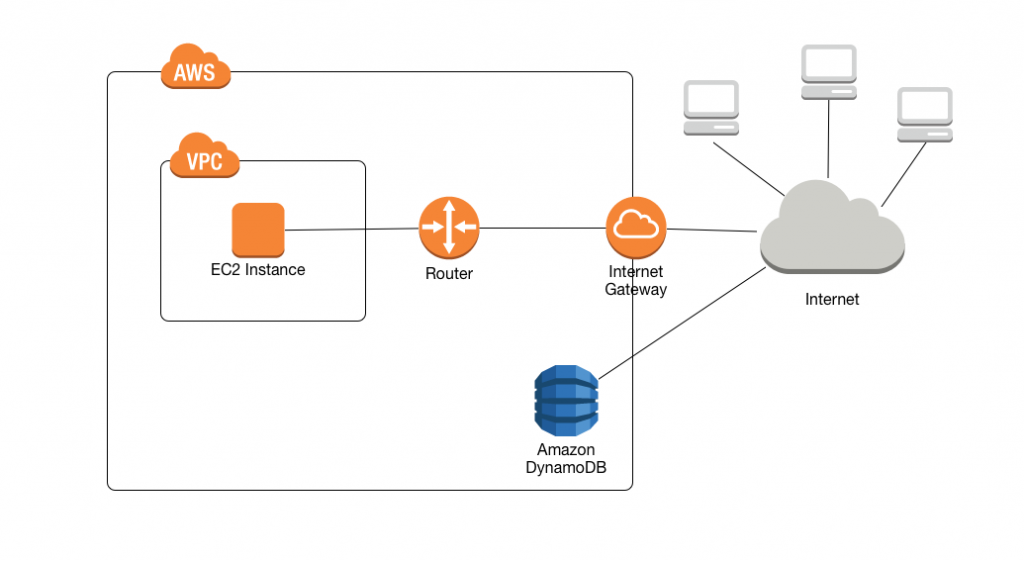
\includegraphics[scale=0.45]{42-aws.png}
%  \caption{A simple Public Cloud configuration using AWS as a provider.}
%\label{aws}
%\end{figure}

\subsection{Getting Set up in AWS}

\justifying
One of the very first things you should do (after creating an account,
that is) is to configure mutli-factor authentication (MFA)\index{multi-factor authentication}.

\justifying
Amazon's AWS is one of the more prevalent cloud providers in terms of
popularity and simultaneously mature and ever-expanding feature set.

\subsection{Credentials}
\justifying
Amazon Web Services (AWS) credentials are stored in a hidden directory
in your home directory called ``.aws''. The file
\textasciitilde{}/.aws/credentials should be modified to contain your
AWS access\_id and secret\_key as seen below.

\begin{mybox}{\thetcbcounter: ~/.aws/credentials}
  \lstinputlisting{code/42-infra/aws-creds.txt}
\end{mybox}

\justifying
Do not share this file with other people. Do not check this file into
your GitHub repositories under any circumstances.

\section{Google Cloud Platform (GCP)}

\justifying
Google Cloud Platform (GCP) is a suite of cloud computing services that
runs on the same infrastructure that Google uses internally for its
end-user products. If the
resources we allocate on GCP were a pyramid, the apex of that pyramid
would be a ``project''. A project is made up of the settings, permissions,
and other metadata that describe your application.

single: Google Cloud Platform single: GCP

\justifying
One of the very first things you should do (after creating an account,
that is) is to configure two-factor authentication\index{two-factor authentication}
(2FA)\index{2FA}.

\justifying
At this point you are ready to install the gcloud\index{gcloud} software development
kit (SDK) on your local machine.

\subsection{Credentials}

\justifying
Once the gcloud SDK is installed, you are ready to set up local
credentials that allow interaction between your machine and the GCP
application programming interface (API). In other words, Google hosts a
server that you can exchange commands with to configure your GCP
projects from your local CLI.

\justifying
GCP credentials are stored in the directory
\textasciitilde{}/.config/gcloud as a JSON file. Do not share this file
with other people. Do not check this file into your GitHub repositories
under any circumstances.

\clearpage
\subsection{Directory Structure}

\justifying
Relevant folders and files related to our build pipeline are shown
below. The users home directory and workspace subdirectory is implied
and removed from the diagram for clarity.

\begin{figure}[!htb]
  
\begin{tikzpicture}[>=latex,line join=bevel,]
  \pgfsetlinewidth{1bp}
%%
\pgfsetcolor{black}
  % Edge: framework -> dotcfg
  \draw [->] (168.11bp,215.7bp) .. controls (163.74bp,207.64bp) and (158.44bp,197.89bp)  .. (148.79bp,180.1bp);
  % Edge: framework -> aws
  \draw [->] (186.89bp,215.7bp) .. controls (191.26bp,207.64bp) and (196.56bp,197.89bp)  .. (206.21bp,180.1bp);
  % Edge: dotcfg -> gcloud
  \draw [->] (139.5bp,143.7bp) .. controls (139.5bp,135.98bp) and (139.5bp,126.71bp)  .. (139.5bp,108.1bp);
  % Edge: gcloud -> sdo
  \draw [->] (139.5bp,71.697bp) .. controls (139.5bp,63.983bp) and (139.5bp,54.712bp)  .. (139.5bp,36.104bp);
  % Node: framework
\begin{scope}
  \definecolor{strokecol}{rgb}{0.0,0.0,0.0};
  \pgfsetstrokecolor{strokecol}
  \draw (251.5bp,252.0bp) -- (248.5bp,256.0bp) -- (227.5bp,256.0bp) -- (224.5bp,252.0bp) -- (103.5bp,252.0bp) -- (103.5bp,216.0bp) -- (251.5bp,216.0bp) -- cycle;
  \draw (177.5bp,234.0bp) node {devsecops\_tactical};
\end{scope}
  % Node: dotcfg
\begin{scope}
  \definecolor{strokecol}{rgb}{0.0,0.0,0.0};
  \pgfsetstrokecolor{strokecol}
  \draw (170.0bp,180.0bp) -- (167.0bp,184.0bp) -- (146.0bp,184.0bp) -- (143.0bp,180.0bp) -- (109.0bp,180.0bp) -- (109.0bp,144.0bp) -- (170.0bp,144.0bp) -- cycle;
  \draw (139.5bp,162.0bp) node {.config};
\end{scope}
  % Node: aws
\begin{scope}
  \definecolor{strokecol}{rgb}{0.0,0.0,0.0};
  \pgfsetstrokecolor{strokecol}
  \draw (242.5bp,180.0bp) -- (239.5bp,184.0bp) -- (218.5bp,184.0bp) -- (215.5bp,180.0bp) -- (188.5bp,180.0bp) -- (188.5bp,144.0bp) -- (242.5bp,144.0bp) -- cycle;
  \draw (215.5bp,162.0bp) node {.aws};
\end{scope}
  % Node: gcloud
\begin{scope}
  \definecolor{strokecol}{rgb}{0.0,0.0,0.0};
  \pgfsetstrokecolor{strokecol}
  \draw (169.5bp,108.0bp) -- (166.5bp,112.0bp) -- (145.5bp,112.0bp) -- (142.5bp,108.0bp) -- (109.5bp,108.0bp) -- (109.5bp,72.0bp) -- (169.5bp,72.0bp) -- cycle;
  \draw (139.5bp,90.0bp) node {gcloud};
\end{scope}
  % Node: sdo
\begin{scope}
  \definecolor{strokecol}{rgb}{0.0,0.0,0.0};
  \pgfsetstrokecolor{strokecol}
  \draw (279.0bp,36.0bp) -- (0.0bp,36.0bp) -- (0.0bp,0.0bp) -- (279.0bp,0.0bp) -- cycle;
  \draw (139.5bp,18.0bp) node {secdevops-my-proj-000101-420240.json};
\end{scope}
%
\end{tikzpicture}


  \caption{IaC related files and folders.}
\label{infra}
\end{figure}

%
\begin{tikzpicture}[>=latex,line join=bevel,]
  \pgfsetlinewidth{1bp}
%%
\pgfsetcolor{black}
  % Edge: home -> devsecops
  \draw [->] (54.172bp,234.0bp) .. controls (61.803bp,234.0bp) and (70.527bp,234.0bp)  .. (89.778bp,234.0bp);
  % Edge: devsecops -> ansible
  \draw [->] (195.15bp,252.13bp) .. controls (209.13bp,258.01bp) and (224.61bp,264.51bp)  .. (247.83bp,274.27bp);
  % Edge: devsecops -> packer
  \draw [->] (212.11bp,234.0bp) .. controls (221.69bp,234.0bp) and (231.39bp,234.0bp)  .. (250.5bp,234.0bp);
  % Edge: devsecops -> aws
  \draw [->] (173.51bp,215.92bp) .. controls (194.73bp,198.09bp) and (227.33bp,170.69bp)  .. (258.92bp,144.14bp);
  % Edge: packer -> adh
  \draw [->] (312.74bp,246.25bp) .. controls (324.62bp,250.98bp) and (338.41bp,256.36bp)  .. (351.0bp,261.0bp) .. controls (364.79bp,266.09bp) and (380.06bp,271.41bp)  .. (403.23bp,279.29bp);
  % Edge: packer -> gdh
  \draw [->] (312.6bp,234.0bp) .. controls (321.04bp,234.0bp) and (330.68bp,234.0bp)  .. (350.84bp,234.0bp);
  % Edge: aws -> main
  \draw [->] (308.74bp,136.66bp) .. controls (321.45bp,141.74bp) and (336.97bp,147.82bp)  .. (351.0bp,153.0bp) .. controls (363.38bp,157.57bp) and (376.94bp,162.32bp)  .. (398.82bp,169.8bp);
  % Edge: aws -> out
  \draw [->] (308.78bp,126.0bp) .. controls (329.01bp,126.0bp) and (357.52bp,126.0bp)  .. (391.85bp,126.0bp);
  % Edge: aws -> tfvars
  \draw [->] (308.74bp,115.34bp) .. controls (321.45bp,110.26bp) and (336.97bp,104.18bp)  .. (351.0bp,99.0bp) .. controls (355.86bp,97.207bp) and (360.91bp,95.385bp)  .. (375.76bp,90.131bp);
  % Edge: aws -> var
  \draw [->] (293.69bp,107.73bp) .. controls (305.74bp,89.464bp) and (326.53bp,61.743bp)  .. (351.0bp,45.0bp) .. controls (356.67bp,41.118bp) and (362.96bp,37.745bp)  .. (379.0bp,30.869bp);
  % Node: home
\begin{scope}
  \definecolor{strokecol}{rgb}{0.0,0.0,0.0};
  \pgfsetstrokecolor{strokecol}
  \draw (54.0bp,252.0bp) -- (51.0bp,256.0bp) -- (30.0bp,256.0bp) -- (27.0bp,252.0bp) -- (0.0bp,252.0bp) -- (0.0bp,216.0bp) -- (54.0bp,216.0bp) -- cycle;
  \draw (27.0bp,234.0bp) node {/home};
\end{scope}
  % Node: devsecops
\begin{scope}
  \definecolor{strokecol}{rgb}{0.0,0.0,0.0};
  \pgfsetstrokecolor{strokecol}
  \draw (212.0bp,252.0bp) -- (209.0bp,256.0bp) -- (188.0bp,256.0bp) -- (185.0bp,252.0bp) -- (90.0bp,252.0bp) -- (90.0bp,216.0bp) -- (212.0bp,216.0bp) -- cycle;
  \draw (151.0bp,234.0bp) node {/home/devsecops};
\end{scope}
  % Node: ansible
\begin{scope}
  \definecolor{strokecol}{rgb}{0.0,0.0,0.0};
  \pgfsetstrokecolor{strokecol}
  \draw (315.0bp,306.0bp) -- (312.0bp,310.0bp) -- (291.0bp,310.0bp) -- (288.0bp,306.0bp) -- (248.0bp,306.0bp) -- (248.0bp,270.0bp) -- (315.0bp,270.0bp) -- cycle;
  \draw (281.5bp,288.0bp) node {ansible};
\end{scope}
  % Node: packer
\begin{scope}
  \definecolor{strokecol}{rgb}{0.0,0.0,0.0};
  \pgfsetstrokecolor{strokecol}
  \draw (312.5bp,252.0bp) -- (309.5bp,256.0bp) -- (288.5bp,256.0bp) -- (285.5bp,252.0bp) -- (250.5bp,252.0bp) -- (250.5bp,216.0bp) -- (312.5bp,216.0bp) -- cycle;
  \draw (281.5bp,234.0bp) node {packer};
\end{scope}
  % Node: aws
\begin{scope}
  \definecolor{strokecol}{rgb}{0.0,0.0,0.0};
  \pgfsetstrokecolor{strokecol}
  \draw (308.5bp,144.0bp) -- (305.5bp,148.0bp) -- (284.5bp,148.0bp) -- (281.5bp,144.0bp) -- (254.5bp,144.0bp) -- (254.5bp,108.0bp) -- (308.5bp,108.0bp) -- cycle;
  \draw (281.5bp,126.0bp) node {aws};
\end{scope}
  % Node: adh
\begin{scope}
  \definecolor{strokecol}{rgb}{0.0,0.0,0.0};
  \pgfsetstrokecolor{strokecol}
  \draw (457.5bp,306.0bp) -- (403.5bp,306.0bp) -- (403.5bp,270.0bp) -- (457.5bp,270.0bp) -- cycle;
  \draw (430.5bp,288.0bp) node {adh};
\end{scope}
  % Node: gdh
\begin{scope}
  \definecolor{strokecol}{rgb}{0.0,0.0,0.0};
  \pgfsetstrokecolor{strokecol}
  \draw (510.0bp,252.0bp) -- (351.0bp,252.0bp) -- (351.0bp,216.0bp) -- (510.0bp,216.0bp) -- cycle;
  \draw (430.5bp,234.0bp) node {gcp-debian-host.json};
\end{scope}
  % Node: main
\begin{scope}
  \definecolor{strokecol}{rgb}{0.0,0.0,0.0};
  \pgfsetstrokecolor{strokecol}
  \draw (462.0bp,198.0bp) -- (399.0bp,198.0bp) -- (399.0bp,162.0bp) -- (462.0bp,162.0bp) -- cycle;
  \draw (430.5bp,180.0bp) node {main.tf};
\end{scope}
  % Node: out
\begin{scope}
  \definecolor{strokecol}{rgb}{0.0,0.0,0.0};
  \pgfsetstrokecolor{strokecol}
  \draw (469.0bp,144.0bp) -- (392.0bp,144.0bp) -- (392.0bp,108.0bp) -- (469.0bp,108.0bp) -- cycle;
  \draw (430.5bp,126.0bp) node {output.tf};
\end{scope}
  % Node: tfvars
\begin{scope}
  \definecolor{strokecol}{rgb}{0.0,0.0,0.0};
  \pgfsetstrokecolor{strokecol}
  \draw (498.0bp,90.0bp) -- (363.0bp,90.0bp) -- (363.0bp,54.0bp) -- (498.0bp,54.0bp) -- cycle;
  \draw (430.5bp,72.0bp) node {terraform.tfvars};
\end{scope}
  % Node: var
\begin{scope}
  \definecolor{strokecol}{rgb}{0.0,0.0,0.0};
  \pgfsetstrokecolor{strokecol}
  \draw (482.0bp,36.0bp) -- (379.0bp,36.0bp) -- (379.0bp,0.0bp) -- (482.0bp,0.0bp) -- cycle;
  \draw (430.5bp,18.0bp) node {variables.tf};
\end{scope}
%
\end{tikzpicture}



%\part{DevSecOps} % part 5
%\chapter{The Lab}


\includegraphics[scale=0.20]{images/milky-way-984050_1920.jpg}
\justify{}
We've reached the point where it's time to assemble all our functional
blocks into a proper lab using resources of a cloud service provider.

\section{Getting Started}

\subsection{Setting up AWS}
\justify{}
Establish an AWS account.

\subsection{Install Docker}
\justify{}
Install Docker on your local machine. Create a Dockerfile and
docker-compose.yml.

\subsection{Configure Project Repository}
\justify{}
Create a GitHub repo for our project. Clone the repo. Copy the
Dockerfile and docker-compose.yml into the new project directory. Create
a branch. Commit the files to the branch and push to repo on GitHub.
Merge the branch, then do a pull to sync your local clone.

\subsection{Configure Testing}
\justify{}
Walk through the steps of adding GitHub Actions that will validate the
Terraform we will be writing to establish our lab infrastructure.

\section{Infrastructure}

\subsection{Lab Diagram}
\justify{}
Let's take a look at the lab environment we intend to create.

\subsection{Add a Makefile}
\justify{}
Add a Makefile that will respond to the ``make docker'' command.

\subsection{Create a Host with Packer}

\subsection{Write Some Terraform Files}

\subsection{Applications}

\subsection{Python Application}

\subsection{Extras}

\subsection{Add a Firewall}
\justify{}
Every keep needs walls around the castle to stop the bad guys from
getting in. The Palo Alto VM-300 series firewall is available as an
image that can be installed in AWS or GCP as desired.


% backmatter: appendix, bibliography, index, postface
\backmatter{}
\printindex
\nocite{*}
\bibliography{backmatter/mybib.bib}
\bibliographystyle{plain}
\chapter*{About the Author}
\addcontentsline{toc}{chapter}{About the Author}
\vspace{5mm}

\justify{}
Franklin Diaz is a Computer Scientist and lifelong computer hobbyist. He
spent 14 years as a Software Engineer, testing and developing Motorola's
CDMA cellular base station products. He spent five years Salesforce where
he was on the Security Detection Engineering team doing security log
aggregation and Data Engineering to augment and enhance the detection
capabilities of the Blue Team.

\justify{}
Most recently he is at Palo Alto Networks where he works on the Professional
Services Team as a Principal Engineer with a focus on automation, Public
Cloud solutions and Continuous Integration and Deployment. He is also the
lead organizer for the BSides Indy security conference in Indianapolis,
Indiana.

\justify{}
His education includes a Bachelor of Science in Computer Science from
Roosevelt University, a Master of Science degree in Computer Information
Systems from Northwestern University, and a Master of Science degree in
Network Security \& Network Engineering from DePaul University.
\vspace{5mm}



%%% front cover, spline, back cover
% front_cover
\end{document}
